\documentclass[dissertacao,brazil]{ThesisPUC}

%%%%%%%%%%%%%%%%%%%%%%%%%%%%%%%%%%%%%%%%%%%%%%%%%%%%%%%%%%%%%%%%%%%%%%%%%%%%%%%%

\usepackage{graphicx}
\usepackage{amsmath}

%%%%%%%%%%%%%%%%%%%%%%%%%%%%%%%%%%%%%%%%%%%%%%%%%%%%%%%%%%%%%%%%%%%%%%%%%%%%%%%%

\newcommand{\Rset}{\mathbb{R}}
\newcommand{\Zset}{\mathbb{Z}}



%%%%%%%%%%%%%%%%%%%%%%%%%%%%%%%%%%%%%%%%%%%%%%%%%%%%%%%%%%%%%%%%%%%%%%%%%%%%%%%%

\autor{Daniel da Rosa Marques}
\autorR{Marques, Daniel da Rosa}
\orientador{Eduardo Sany Laber}
\orientadorR{Eduardo Sany Laber}
\titulo{Um Meta-classificador para Geração de Rankings}
\subtitulo{}
\dia{22} \mes{Junho} \ano{2015}

\cidade{Rio de Janeiro}
\CDD{510}
\departamento{Informática}
\programa{Otimização e Raciocínio Automático}
\centro{Centro T\'{e}cnico Cient\'{i}fico}
\universidade{Pontif\'{i}cia Universidade Cat\'{o}lica do Rio de Janeiro}
\uni{PUC--Rio}


%%%%%%%%%%%%%%%%%%%%%%%%%%%%%%%%%%%%%%%%%%%%%%%%%%%%%%%%%%%%%%%%%%%%%%%%%%%%%%%%

\banca{
  \membrodabanca{Membro banca 1}{Instituição}
  \coordenador{}
}


%%%%%%%%%%%%%%%%%%%%%%%%%%%%%%%%%%%%%%%%%%%%%%%%%%%%%%%%%%%%%%%%%%%%%%%%%%%%%%%%

\curriculo{.
Graduou-se em Engenharia Eletrônica e da Computação na Universidade Federal do Rio de Janeiro. Trabalhou com desenvolvimento de soluções de informática em diversas empresas.
}


%%%%%%%%%%%%%%%%%%%%%%%%%%%%%%%%%%%%%%%%%%%%%%%%%%%%%%%%%%%%%%%%%%%%%%%%%%%%%%%%

\agradecimentos{%
Ao meu orientador Professor Eduardo Sany Laber pelo apoio e orientação no desenvolvimento deste trabalho.

À CAPES e \`{a} PUC--Rio, pelos aux\'{i}lios concedidos, os quais possibilitaram a realização deste trabalho.

Ao Félix Ribeiro, minha maior fonte de inspiração e coragem, sem ele nada disso seria possível.

A minha mãe, irm\~{a} e fam\'{i}lia, sempre na torcida.

Aos meus colegas da PUC--Rio, que também me ajudaram nessa jornada.

Aos funcionários do departamento de Informática pela a ajuda de costume.
}


%%%%%%%%%%%%%%%%%%%%%%%%%%%%%%%%%%%%%%%%%%%%%%%%%%%%%%%%%%%%%%%%%%%%%%%%%%%%%%%%

\chaves{%
  \chave{Aprendizado de Máquina}%
  \chave{Ranking}%
}

\resumo{
Em construção.
}


%%%%%%%%%%%%%%%%%%%%%%%%%%%%%%%%%%%%%%%%%%%%%%%%%%%%%%%%%%%%%%%%%%%%%%%%%%%%%%%%

\chavesuk{
  \chave{Machine Learning}%
  \chave{Ranking}%
}

\titulouk{A Meta-classifier for Ranking}

\resumouk{%
Under Construction.
}


%%%%%%%%%%%%%%%%%%%%%%%%%%%%%%%%%%%%%%%%%%%%%%%%%%%%%%%%%%%%%%%%%%%%%%%%%%%%%%%%

\modotabelas{figtab} % nada, fig, tab ou figtab

%%%%%%%%%%%%%%%%%%%%%%%%%%%%%%%%%%%%%%%%%%%%%%%%%%%%%%%%%%%%%%%%%%%%%%%%%%%%%%%%

\epigrafe{%
???
}
\epigrafeautor{???}
\epigrafelivro{???}

%%%%%%%%%%%%%%%%%%%%%%%%%%%%%%%%%%%%%%%%%%%%%%%%%%%%%%%%%%%%%%%%%%%%%%%%%%%%%%%%

\begin{document}

\chapter{Introdução}

Existem diversas tarefas importantes que o homem costuma desempenhar melhor do que a máquina.
Entretanto, o aprendizado de máquina tem sido utilizado com sucesso para resolver algumas destas.
Especilamente aquelas que exigem o processamento de uma grande quantidade de dados, o que seria inviável ser feito manualmente.
Exemplos destas tarefas são reconhecimento de imagens, tradução automática de idiomas, reconhecimento de fala, movimentação de autômatos, sistemas de recomendação, entre outras.

As soluções para algumas dessas tarefas utilizam conceitos de \textit{ranking}.
Por exemplo, em sistemas de recomendação \textit{ranking} é utilizado para criar listas de documentos com base naqueles vistos anteriormente por um usuário.

Motivado por isso, este trabalho se concentra em tarefas de \textit{ranking}.
Durante o projeto, criamos um meta-classificador para aprendizado de máquina supervisionado adequado para este tipo de tarefa.
Este meta-classificador é capaz de utilizar internamente qualquer tipo de classificador encontrado na literatura.

\section{Descrição do Problema}

Para entender o problema de \textit{ranking} no qual este trabalho se concentra, considere um exemplo onde temos uma rede \textit{R} com \textit{k} nódos.
Imagine que esta rede eventualmente pode apresentar falhas em seus nódos, sendo que cada falha pode causar sérios danos à operação da rede.
Para corrigir-las é necessário faze-lo diretamente no nódo afetado pela falha.
Além disso, para corrigir uma falha rapidamente, é necessário determinar logo onde ela ocorreu.
Para tanto poderíamos verificar simultaneamente todos os \textit{k} nódos, por exemplo enviando equipes até os locais.
Entretanto o custo do deslocamento até um dos nódos é muito elevado, sendo inviável checar toda a rede sempre que ocorre uma falha.

No âmbito do aprendizado de máquina tradicional os nódos da rede podem ser traduzidos em classes.
Além disso, temos diversas estatísticas e medições sobre o estado da rede \textit{R} ao longo do tempo.
Estas podem ser utilizadas como atributos.
Gostaríamos então de identificar automaticamente o nódo onde uma falha ocorre, provavelmente usando um classificador.

Tendo em vista a dificuldade de gerar essa informação com absoluta precisão, uma solução razoável é construir uma lista dos nódos mais prováveis onde a falha ocorreu.
Quanto mais próximo da primeira posição da lista estiver o nódo verdadeiro, menor será o custo de reparo da rede.
Embora o meta-classificador desenvolvido possa ser utilizado para tarefas de \textit{ranking} de propósito geral, o problema definido acima será usado ao longo do trabalho como tarefa principal.

\section{Contribuições}

Neste trabalho propomos um método para geração de \textit{rankings} que é capaz de utilizar qualquer tipo de classificador para esta tarefa.
De fato, como já citamos, da forma que foi implementado ele funciona como um meta-classificador.

O método elimina ruído sucessivamente do conjunto de treino à medida que a lista de saída é construída.
Isso foi feito por meio de filtragens aplicadas aos dados, que removem intâncias de classes já incluídas na lista.
Desta forma, os classificadores internos do meta-classificador são treinados com conjuntos de treino filtrados de formas diferentes.
Isto é, cada classificador gera um modelo único do qual algumas classes foram retiradas.
Cada modelo é utilizado então para gerar um único elemento da lista de saída.
Veremos que para classificar diversas intâncias, com listas de saída diferentes, uma grande quantidade de classificadores precisa ser gerada.
Por exemplo, se o conjunto de dados tem sete classes diferentes o meta-classificador pode vir a ter mais de cem classificadores internos.

Além disso, o método foi desenvolvido em duas versões: estática e dinâmica.
As duas versões diferem no momento no qual os classificadores internos são treinados.

A primeira versão treina todos os classificadores internos possíveis a priori.
Esta abordagem exigiu um tempo de treinamento maior.
Isto por que, dependendo do conjunto de dados, a quantidade de classificadores possíveis pode ser grande.
Todavia, uma vez que todos os classificadores foram treinados, o tempo de classificação das intâncias foi análogo ao de um classificador comum.

A segunda versão treina os classificadores à medida que o \textit{ranking} é gerado.
Nesta versão, somente os classificadores necessários para construção daquela lista são treinados.
Com isso o método dinâmico conseguiu tempos de treinamento melhores do que a versão anteriror.
Por outro lado, seus tempos de classificação foram piores visto que o modelo é treinado durante a construção da lista de saída.

Para avaliar os resultados de problemas como o da rede, desenvolvemos para este trabalho métricas denominadas \textit{k-acurácias}.
Onde \textit{k} denota a posição da lista de saída a qual cada uma se refere, e.g. a 1-acurácia remete à primeira posição da lista, a 2-acurácia à segunda e assim por diante.
Note que essas métricas refletem o cenário da rede \textit{R} descrito anteriormente.
Considere que equipes são enviadas para corrigir os erros; a 1-acurácia se aplica ao cenário onde uma equipe foi enviada, a 2-acurácia duas equipes e assim por diante.
Portanto essa métricas apontam um melhor resultado quanto mais bem posicionada estiver a classe verdadeira na lista de saída.

O método proposto foi implementado na forma de um meta-classificador.
Este foi programado em Java e utiliza diretamente as classes para aprendizado de máquina do \textit{Framework Weka}.
Com isso o meta-classificador é capaz de utilizar internamente a uma grande quantidade de classificadores diferentes disponíveis nesta ferramenta.

Propomos a utilização de classificadores probabilísticos para criar o \textit{Benchmark} dos testes de performance do método. 
Esses classificadores foram utilizados para construir as listas usadas como base para a avaliação dos modelos.
Isso foi possível pois, eles podem gerar a probabilidade de cada classe para uma dada instância.
A partir desta informação montamos um \textit{ranking} de classes para a instância.

Durante a avaliação do método, executamos e analisamos testes do meta-classificador em combinação com classificadores conhecidos como o SVM, a Árvore de Decisão e o KNN.
Observamos que o metaclassificador destacou-se nos testes com alguns deles, principalmente com a Árvore de Decisão.
Além disso, discutimos os resultados do método quando aplicado à conjuntos de dados reais e sintéticos.
Os tempos de execução também foram analisados.
Dependendo do npumero de classes envolvido o método proposto atinge tempos de execução razoáveis; ainda que mais lentos do que dos classificadores probabilísticos comuns.

\section{Organização da Dissertação}

Os capítulos deste texto estão organizados da forma a seguir.
Primeiro são introduzidos os conceitos necessários para o entendimento do trabalho no Capítulo \ref{chap:conceitosbasicos}.
Em seguida, no Capítulo \ref{chap:metodoproposto} o método é discutido em detalhes.
Depois os experimentos realizados para testar o método são detalhados e seus resultados são discutidos no Capítulo \ref{chap:descricaodostestes}.
Posteriormente, no Capítulo \ref{chap:trabalhosrelacionados}, uma compilação de trabalhos relacionados à este é apresentada.
Por fim, o texto é concluído com nossas considerações finais sobre o trabalho.


\chapter{Conceitos Básicos}
\label{chap:conceitosbasicos}

Aprendizado de máquina é um dos campos de pesquisa da inteligência artificial e por sua vez da ciência da computação.
Esta área de estudos se concentra na pesquisa e desenvolvimento de algoritmos que possam aprender tarefas automaticamente.
Tipicamente estes algoritmos geram um \textit{modelo matemático} partir de um ou mais conjuntos de dados.
O modelo é então responsável por desempenhar a tarefa, ou seja, não é necessário escrever um programa para tanto.
Aprendizado de máquina tem inúmeras aplicações, entre elas podemos citar filtros de spam, reconhecimento ótico de caracteres, motores de busca, visão computacional, entre outras.

\section{Aprendizado Supervisionado}

Aprendizado supervisionado é inspirado na ideia de aprendizado por exemplos.
Isto é, uma grande quantidade de exemplos é fornecida para o algoritmo no intuito de faze-lo aprender.
Todos os exemplos devem ter o mesmo formato.
Cada um deles é composto por dois ou mais atributos, sendo que um dos atributos deve ser o alvo da tarefa de aprendizado.
Os demais atributos devem constituir informações relevantes que permitam ao algoritmo aprender a tarefa.
De forma geral temos que um conjunto com \textit{N} exemplos é da forma $ \{(x_1, y_1), ..., (x_N,\; y_N)\} $ tal que $x_i$ representa o conjunto de atributos informativos do exemplo e $y_i$ é seu atributo alvo.

\begin{figure}[h!]
  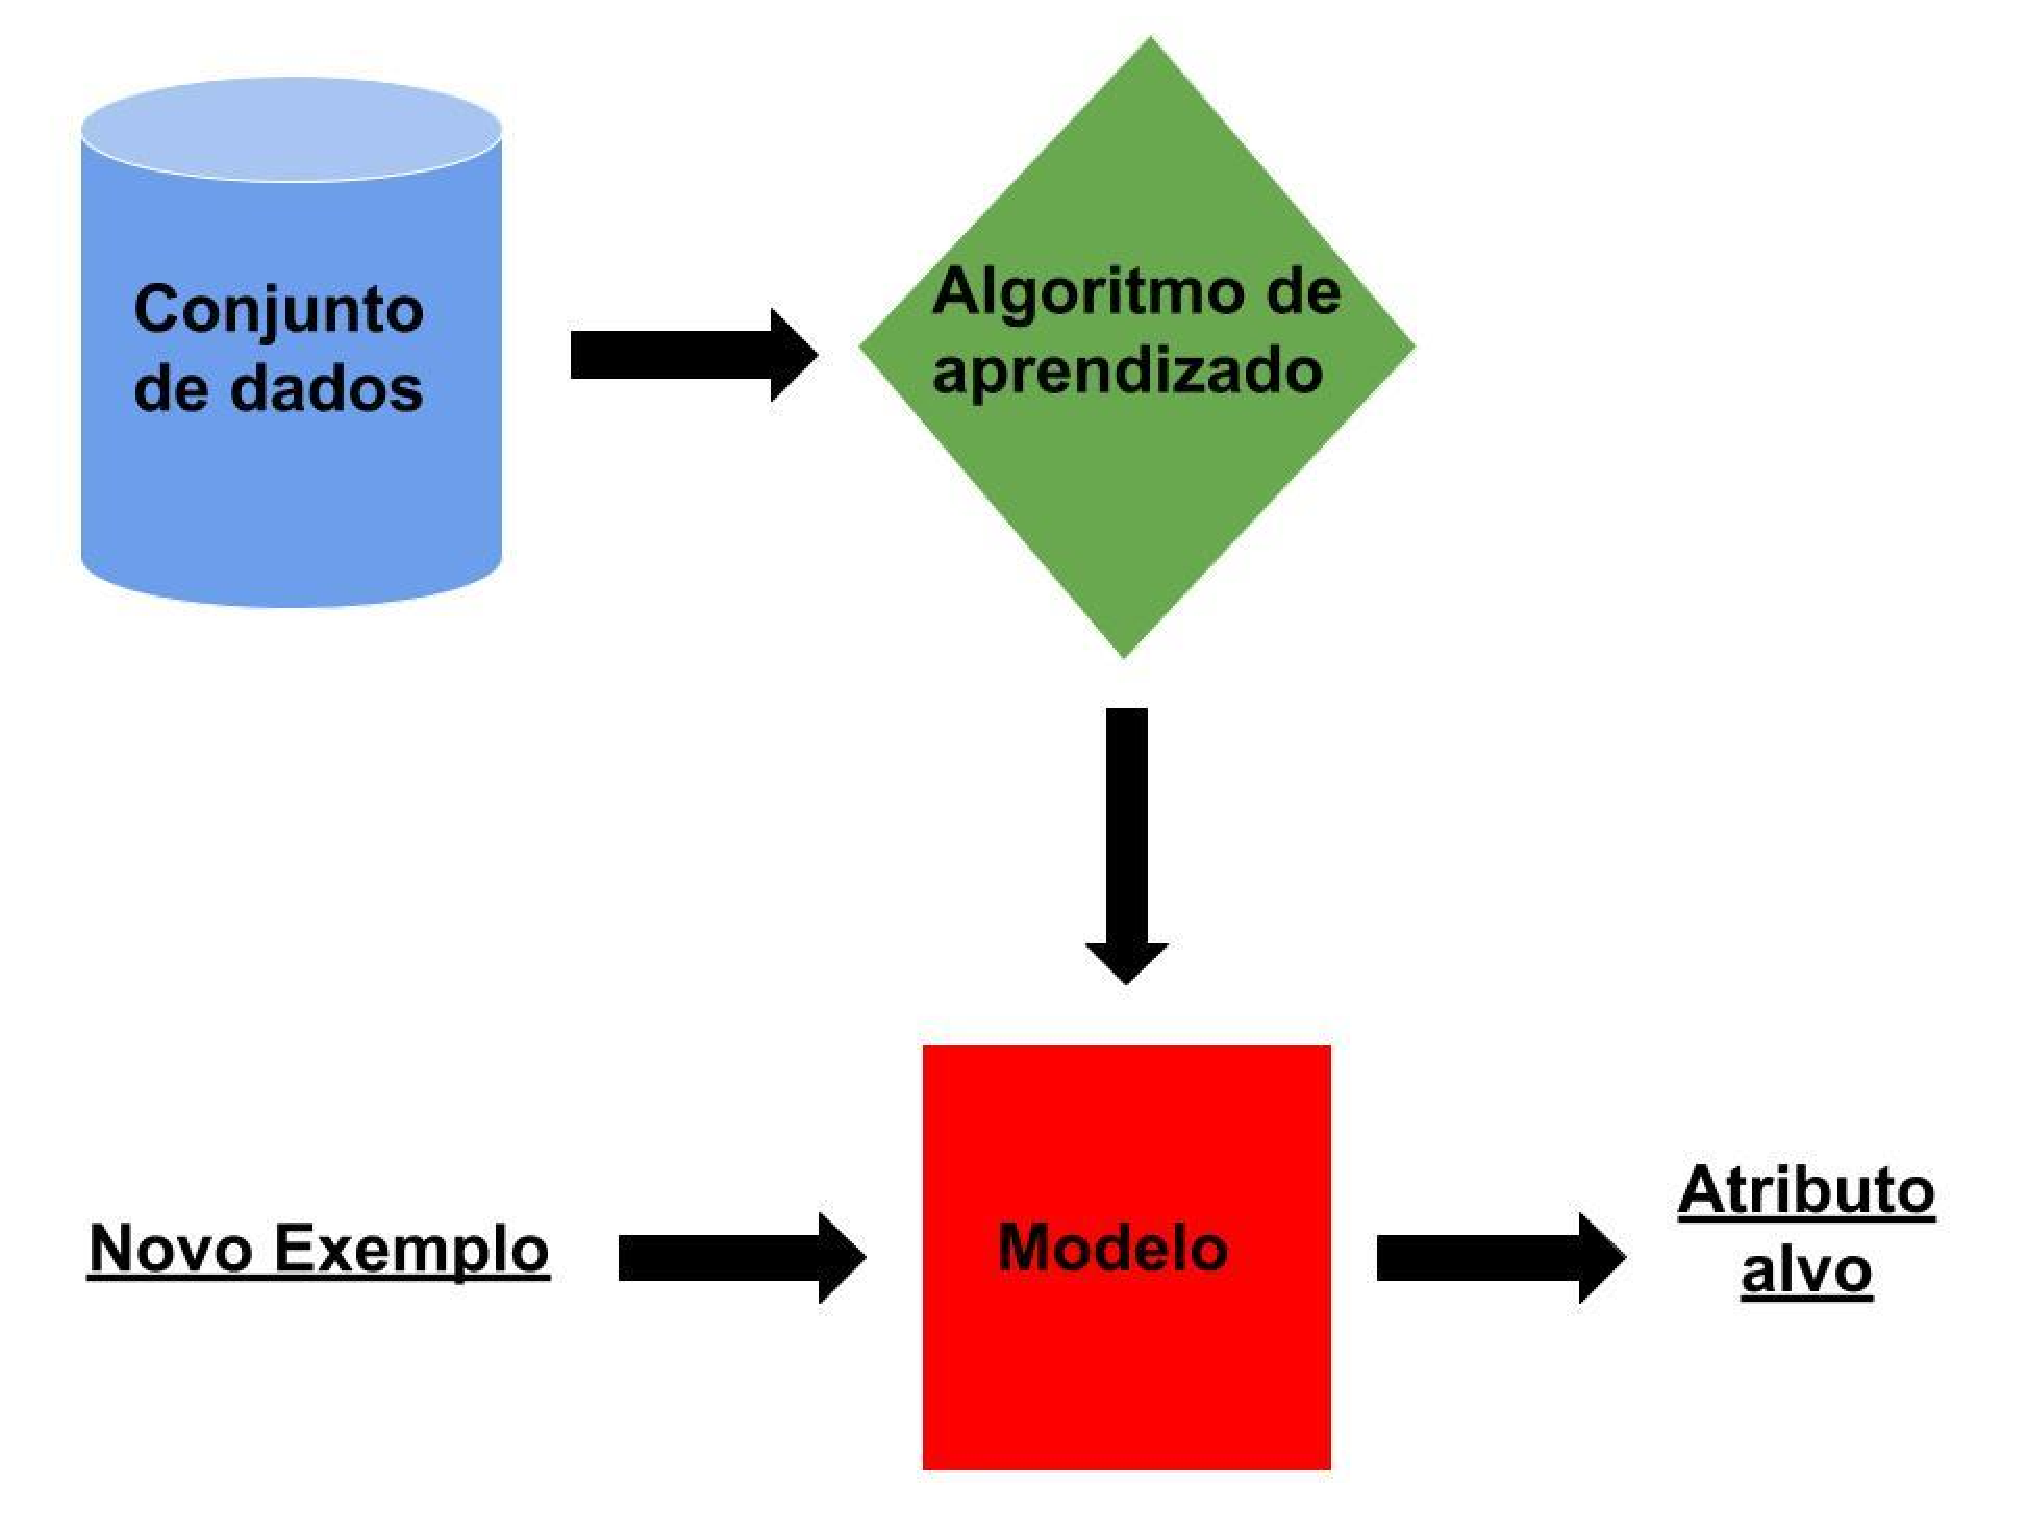
\includegraphics[width=\linewidth]{images/conceitosbasicos01.eps}
  \caption{Fluxo do aprendizado supervisionado para classificação}
  \label{fig:conceitosbasicos01}
\end{figure}

O algoritmo de aprendizado deve gerar uma função $g: X \to Y$, onde \textit{X} é o conjunto de entrada e \textit{Y} o conjunto de saída.
Uma vez que processou os exemplos, o algoritmo gera um modelo que representa a função \textit{g}.
Por fim, dados que ainda não foram vistos, desprovidos do atributo alvo, podem ser submetidos ao modelo.
Com isso, ele pode executar automaticamente a tarefa para a qual foi treinado, e.g. determinar a qual classe o dado inédito pertence.
Veja na figura \ref{fig:conceitosbasicos01} um diagrama que ilustra o processo de aprendizado supervisionado.

Para exemplificar como funciona o aprendizado supervisionado, consideremos o problema da figura \ref{fig:conceitosbasicos02}.
Neste queremos um modelo capaz de diferenciar entre círculos e triângulos.
Ou seja, temos um problema de classificação binária.
Para resolve-lo precisamos de um modelo que funcione como um separador linear.
O algoritmo utilizado para gerar o modelo deve então aprender uma função \textit{f(x)} que mapeia o vetor de entrada \textit{x} em um único valor de saída. Esta função pode ser definida como:

\begin{equation*}

\centering

f(x) =
        \begin{cases}

        1 & \text{se }w \cdot x + b > 0\\
        0 & \text{caso contrário}

        \end{cases}

\end{equation*}

onde,
\begin{itemize}
\item Os valores de saída de \textit{f(x)} representam a resposta do classificador, por exemplo o valor 0 pode indicar um círculo e o valor 1 um trigângulo
\item \textit{x} é um vetor de números reais que representam os valores de atributos de entrada, no exemplo podem ser as coordenadas dos centros de cada círculo e triângulo
\item \textit{w} é um vetor de números reais que representam os pesos conferidos aos atributos pelo algoritmo de aprendizado
\item \textit{b} é uma constante de bias
\end{itemize}

\begin{figure}[h!]
  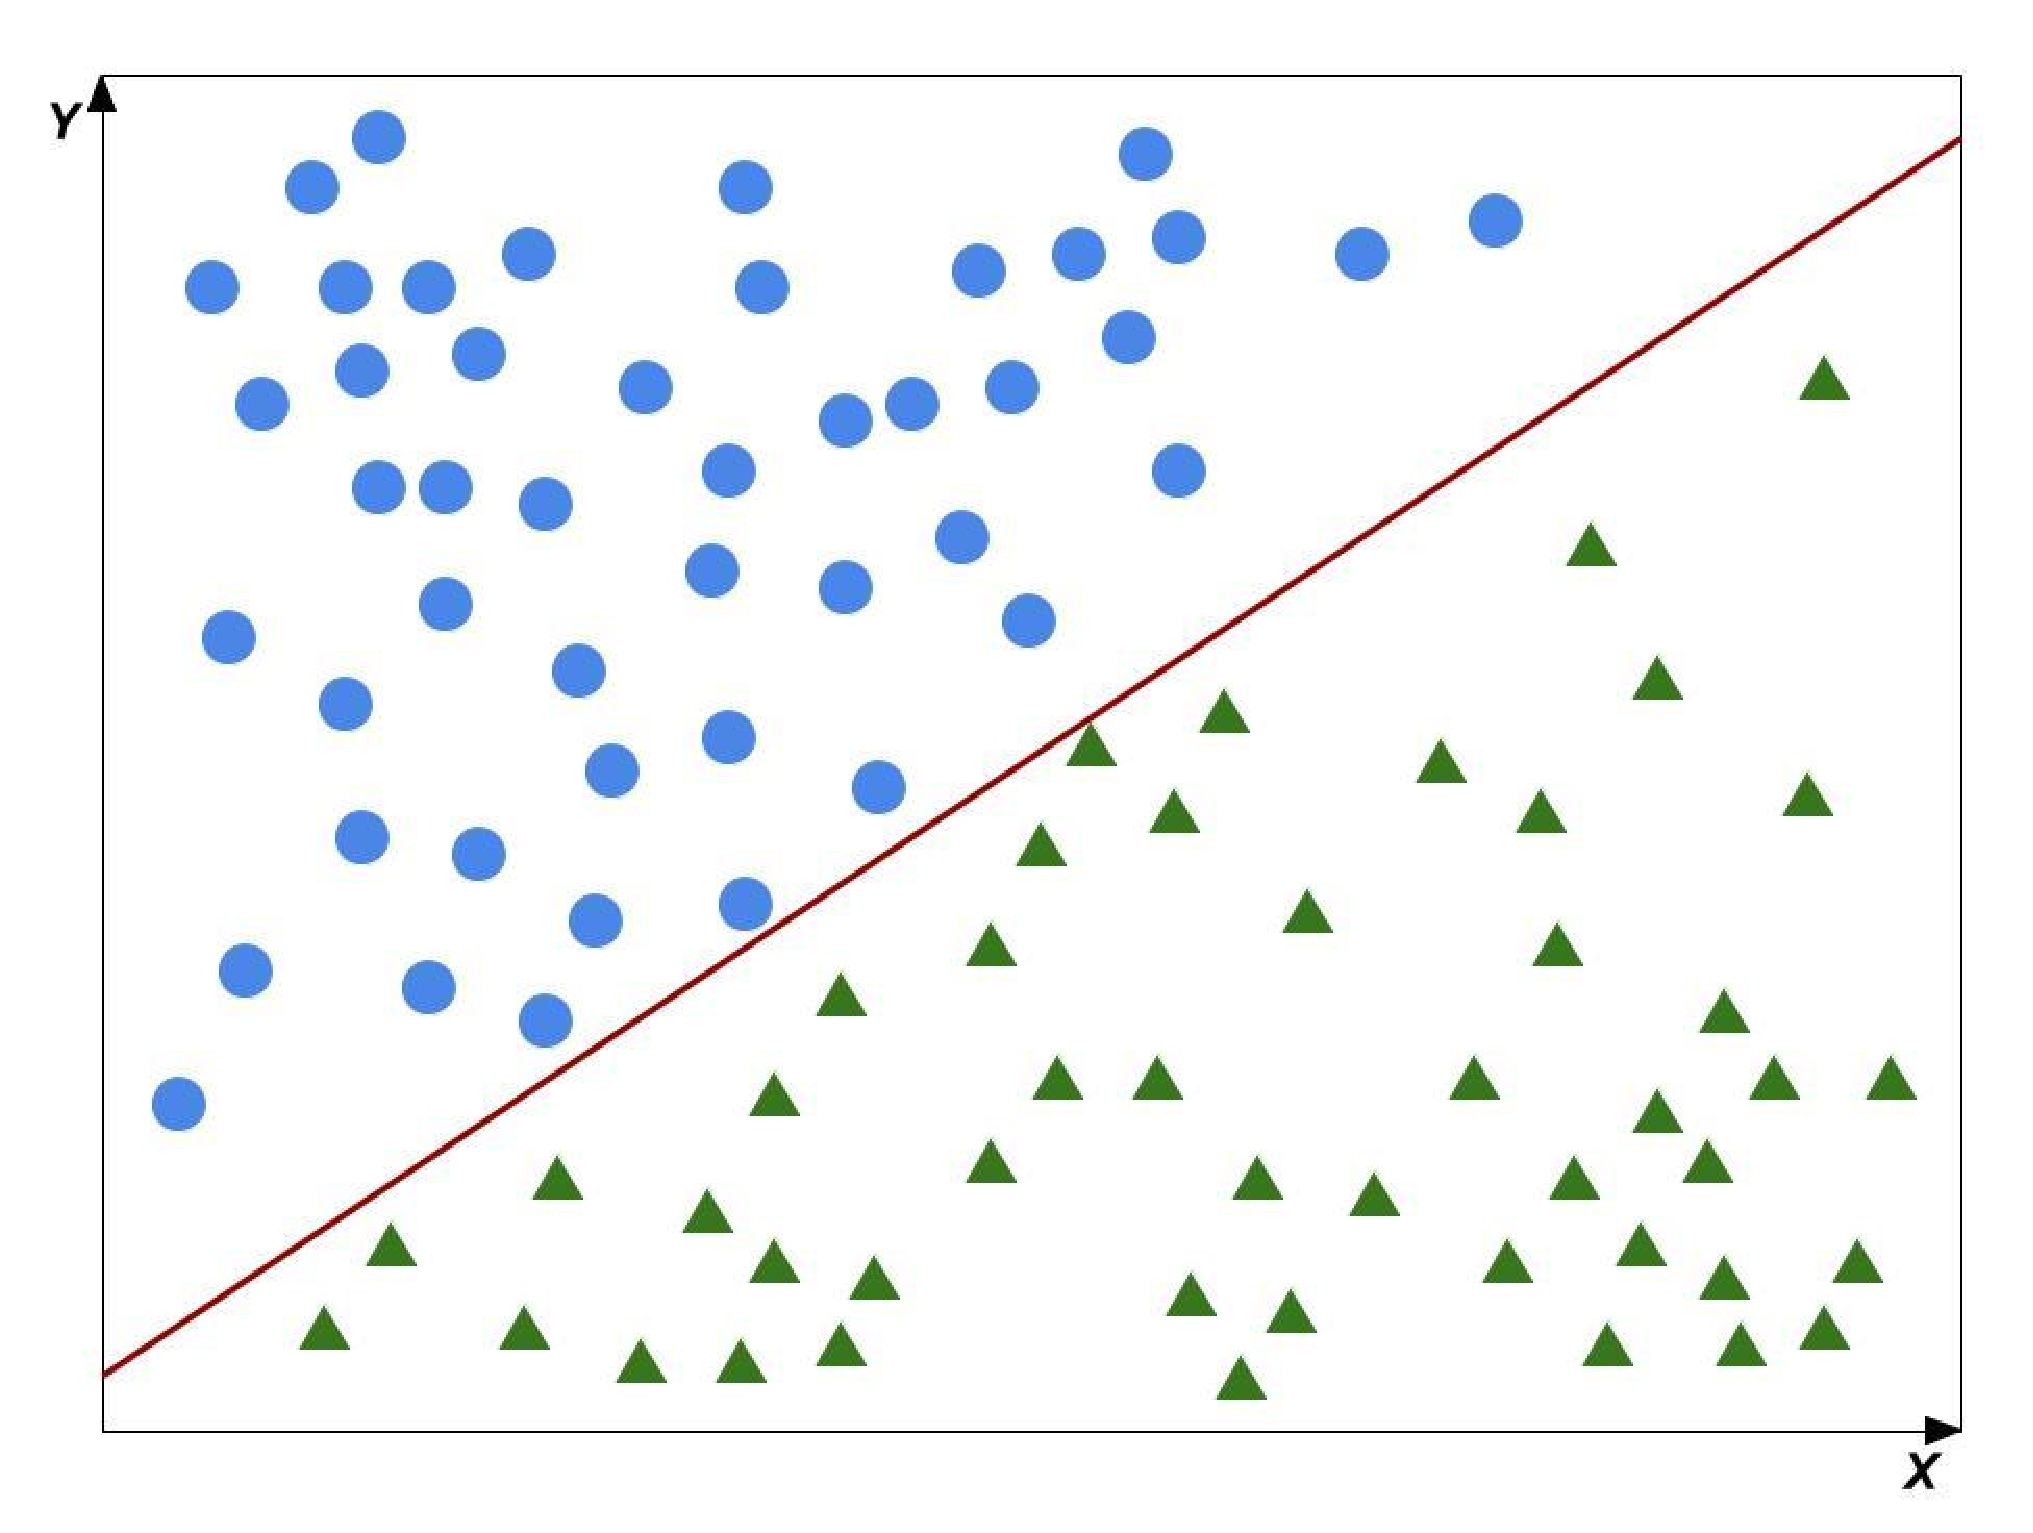
\includegraphics[width=\linewidth]{images/conceitosbasicos02.eps}
  \caption{Exemplo de separador linear}
  \label{fig:conceitosbasicos02}
\end{figure}

Com isso o problema se resume a calcular os valores do vetor de pesos \textit{w}.
Considere que temos disponível os dados dos diversos exemplos de círculos e triângulos vistos na figura.
A os exemplos envolvidos no processo de aprendizado são denominados \textit{conjunto de dados}.
Cada exemplo contém as coordenadas \textit{(x,y)} mais o valor da classe (circulo ou triângulo).
O algoritmo supervisionado simples proposto a seguir para resolver este problema é baseado no perceptron.
\\

\hline
\begin{center}
\textbf{Algoritmo de aprendizado}
\end{center}
\hline
\hfill \break
Inicializa o vetor \textit{w} com valores aleatórios
Para cada exemplo do conjunto de dados:
\begin{enumerate}
\item Calcula o valor de saída de \textit{f(x)}
\item Calcula a diferença entre o valor obtido e o real (retirado do exemplo) 
\item Corrige os valores do vetor de pesos \textit{w} por valores proporcionais a esta diferença
\end{enumerate}
\hline
\hfill \break

No exemplo todos os atributos eram números reais.
Porém, com a utilização de outros algoritmos os atributos podem ser de diversos tipos: nominal (uma lista de classes), numérico (um número inteiro ou real), uma data, etc.

As tarefas de aprendizado supervisionado mais clássicas são a classificação, vista no exemplo, e a regressão.
Quando o alvo da tarefa é um atributo nominal dizemos que esta é uma classificação e quando é um número real dizemos que é uma regressão.
Todavia existem outras tarefas nas quais o aprendizado supervisionado pode ser empregado, como é o caso do \textit{ranking}.

Em um problema de \textit{ranking}, queremos que o modelo gere uma lista ordenada de classes como saída.
Para tanto, os exemplos fornecidos ao algoritmo de aprendizado também devem ter uma lista ordenada de classes ao invés de um atributo classe único.
Isto é, em cada exemplo $ (x_i,\; y_i) $ temos que $y_i$ é da forma $ [l_1, l_2, ..., l_k] $ onde \textit{k} representa o número total de classes. Veremos em outros capítulos que esta dissertação de mestrado se concentra em problemas desse tipo.

\subsection{Algoritmos de aprendizado}

O perceptron, cujo princípio de funcionamento é o mesmo do algoritmo apresentado anteriormente, é um algoritmo de aprendizado supervisionado clássico encontrado na literatura \cite{Rosenblatt}.
Ele serviu como base para métodos mais complexos como por exemplo o \textit{Support Vector Machine} (SVM) \cite{Chang}.
Entretanto, existem algoritmos baseados em outros princípios.
Quando realizamos os experimentos deste trabalho procuramos comparar classificadores com princípios de funcionamento distintos.
Foram usados os classificadores: SVM, \textit{Naive Bayes} \cite{Murphy}, Arvore de Decisão \cite{Quinlan}, \textit{Random Forest} \cite{Breiman} e \textit{k-nearest neighbors} (KNN) \cite{Duda}.
Descreveremos a seguir de forma breve como esses algoritmos funcionam.

Como foi dito, o SVM é derivado diretamente do Perceptron.
Ambos são classificadores binários lineares não probabilísticos.
O SVM também pode ser usado para resolver problemas como o da figura \ref{fig:conceitosbasicos02}.
Este classificador considera cada vetor de atributos de entrada \textit{x} com \textit{d} dimensões.
Ele então calcula um hiperplano, com \textit{d-1} dimensões, para separar os pontos no espaço \textit{d}-dimensional dos exemplos.
No exemplo da figura temos que \textit{d} é igual a 2 e portanto o hiperplano é uma reta.
Este calculo ocorre iterativamente, a partir do conjunto de treino, de forma análoga ao algorítimo apresentado anteriormente.
Além disso, o SVM procura encontrar o melhor hiperplano de separação para os pontos, i.e. aquele mais afastado de todos. 
Para tanto ele considera a existência uma \texiit{margem} que representa o afastamento do hiperplano para os pontos.
Por fim ele calcula o hiperplano de margem máxima.

\textit{Naive Bayes} são classificadores probabilísticos baseados no teorema de Bayes.
Este algoritmo cria um modelo de probabilidade condicional que recebe como entrada o vetor $ \textit{x} = (x_1, x_2, ... , x_d) $, com \textit{d} atributos.
Ele assume entretanto que estes atributos de entrada são independentes.
Para classificar uma instância o modelo determina a probabilidade de cada classe $C_i$ possível, dada por $p(C_i|x_1, x_2, ... , x_d)$, com a ajuda do teorema de Bayes.
Por fim, o classificador utiliza as probabilidades para decidir qual classe escolher baseado em uma regra preestabelecida, e.g. a classe mais provável.

As árvores de decisão são modelos de predição que utilizam os atributos de entrada para tomar decisões e desta forma inferir a classe de uma intância.
Sendo assim, as folhas da árvore representam classes enquanto os nódos representam decisões baseadas nos atributos.
De forma geral, para construir um modelo a partir do conjunto de treino, a árvore de decisão escolhe a cada nódo o atributo que melhor divide o conjunto.
Depois que o modelo está pronto, é possível utilizar os atributos de uma nova instância para percorrer a árvore de acordo com as decisões nos nódos.
Com isso chega-se até uma folha que determinará a classe da instância.
Note que tipos distintos de árvore podem utilizar critérios diferentes para a escolha do atributo decisório dos nódos.
O \textit{ Ganho de Informação} por exemplo é empregado nas arvores de decisão do tipo C4.5 (utilizadas nos testes conduzidos neste trabalho).

O \textit{Random Forest} é um método que utiliza um comitê de árvores de decisão para classificação.
Isto é, durante o treinamento o algoritimo cria diversas árvores de decisão que compõem o modelo.
Cada árvore contribui votando em uma classe e no final a classe mais votada é escolhida.
Esse algoritimo utiliza \textit{Bagging} para criar subconjuntos aleatórios do conjunto de treino.
Cada subconjunto é utilizado para treinar uma das árvores de decisão.
Além disso, o \textit{Random Forest} também emprega o \textit{Feature Bagging}, i.e. cada árvore utiliza somente um subgrupo aleatório dos atributos originais no treinamento.

O algoritimo KNN apenas recebe os vetores de atributos de entrada do conjunto de treino em um primeiro momento.
Para classificar uma instância ele simplesmente determina qual é a classe mais frequente entre os \textit{k} exemplos mais próximos, onde \textit{k} é definido pelo usuário.
Este método pode utilizar diferentes métricas de proximidade para determinar os vetores próximos, uma das mais utilizadas é a distância euclidiana.

\subsection{Avaliação de Performance}

Para treinar e avaliar a performance de um algoritmo de aprendizado, tipicamente o conjunto de dados é dividido em dois.
O primeiro, \textit{conjunto de treino}, contém os exemplos que efetivamente serão usados para treinar o algoritmo.
O restante, \textit{conjunto de testes}, é usado para fornecer exemplos inéditos ao modelo.
O resultado obtido quando o conjunto de testes é submetido ao modelo é utilizando para calcular as métricas pertinentes.
Essa divisão de dados é feita para garantir que o modelo foi capaz de generalizar e não apenas decorou o conjunto de dados (\textit{overfitting}).
Note que esta técnica de avaliação acaba por não utilizar uma parte dos dados (conjunto de teste) no treinamento.
Isso pode criar dificuldades quando a quantidade de dados disponível for muito limitada.

Outra forma de avaliação importante é chamada \textit{validação cruzada}.
Neste caso o conjunto de dados é dividido em \textit{k} subconjuntos.
Estes podem ou não manter aproximadamente as mesmas proporções de classes do conjunto de dados original, dependendo do que se deseja fazer.
A partir disso o algoritmo de aprendizado é executado \textit{k} vezes, gerando um modelo diferente por vez.
A cada iteração, aquele modelo é treinado com \textit{k-1} subconjuntos como conjunto de treino e o restante (1 subconjunto) como conjunto de testes.
Desta forma, no decorrer das \textit{k} iterações do treinamento, todos os dados são usados.
Por fim, os resultados de todos os modelos são combinados para gerar as estatísticas finais.

\subsection{Métricas de Avaliação}

Para ilustrar as métricas de avaliação suponha um exemplo onde temos um modelo \textit{M}.
Ele foi treinado para identificar se uma máquina apresenta falha ou não, baseando-se em uma série de medidas recolhidas sobre a mesma (atributos).
Aplicamos então esse modelo à um conjunto de 100 instâncias e obtemos um resultado como o da tabela \ref{tab:positivosenegativos}.

\begin{table}[h!]
  \begin{center}
    \begin{tabular}{ccc}
      \hline
        & \textbf{Real: com falha} & \textbf{Real: sem falha} \\
      \hline

      \textbf{Previsto: com falha} & 5 (\textit{true positive}) & 5 (\textit{false positive}) \\
      \textbf{Previsto: sem falha} & 10 (\textit{false negative}) & 80 (\textit{true negative} )\\

      \hline
    \end{tabular}
    \caption{Resultados do modelo \textit{M}}
    \label{tab:positivosenegativos}
  \end{center}
\end{table}

Os dados da tabela \ref{tab:positivosenegativos} estão separados em \textit{true positive}, \textit{true negative},\textit{false positive} e \textit{false negative}.
Os dois primeiros indicam o número de instâncias corretamente classificadas e o restante a quantidade classificada incorretamente.
A partir desses valores é possível gerar algumas das métricas mais usuais em aprendizado de máquina, as quais apresentaremos nas equações a seguir.

\begin{align*}

\[ \textit{Acurácia} &= \frac{TP+TN}{TP+TN+FP+FN} \] \\
\[ \textit{Precision} &= \frac{TP}{TP+FP} \] \\
\[ \textit{Recall} &= \frac{TP}{TP+FN} \]
\end{align*}

Baseando-se nas equações, temos no exemplo da tabela \ref{tab:positivosenegativos} um valor de \textit{Acurácia} igual a 85 \%, \textit{Precision} igual a 50 \% e \textit{Recall} igual a 33,33 \%.

Notadamente cada uma dessas métricas é mais apropriada em casos distintos.
A \textit{Acurácia} talvez seja a métrica mais instintiva e simples, visto que ela representa a proporção de elementos corretamente classificados.
Mas nem sempre é possível avaliar um modelo da melhor maneira com ela.
Considere por exemplo o caso de um modelo \textit{M'} que simplesmente classifica as instâncias como \textit{sem falha}.
Ele atingiria uma \textit{Acurácia} de 85 \% mas seria incapaz de identificar máquinas com falha.

Para compreender intuitivamente o \textit{Precision} e o \textit{Recall} podemos recorrer à conceitos de \textit{Information Retrieval}.
Neste contexto o \textit{Precision} denota qual proporção dos elementos selecionados pelo modelo realmente são relevantes, no caso do exemplo da tabela \ref{tab:positivosenegativos} máquinas com falha.
Por outro lado, o \textit{Recall} representa qual proporção dos elementos relevantes presentes nos dados foi selecionada pelo modelo.



\chapter{Método Proposto}
\label{chap:metodoproposto}

O método proposto deve receber como entrada um conjunto de treino, a partir do qual um modelo é construído. Quando uma nova instância é recebida este modelo pode ser usado para gerar uma lista ordenada de saída (ranking). Esta lista é composta pelos valores de classe (do conjunto de treino) mais prováveis para aquela instância, de forma que o primeiro valor é o mais provável. 

O método proposto compreende um metaclassificador que por sua vez é composto por um conjunto de classificadores internos. Estes diversos classificadores são empregados em cascata para gerar a lista ordenada de saída. Note que, cada item da lista é dado por apenas um classificador interno. 

\begin{figure}[h!]
  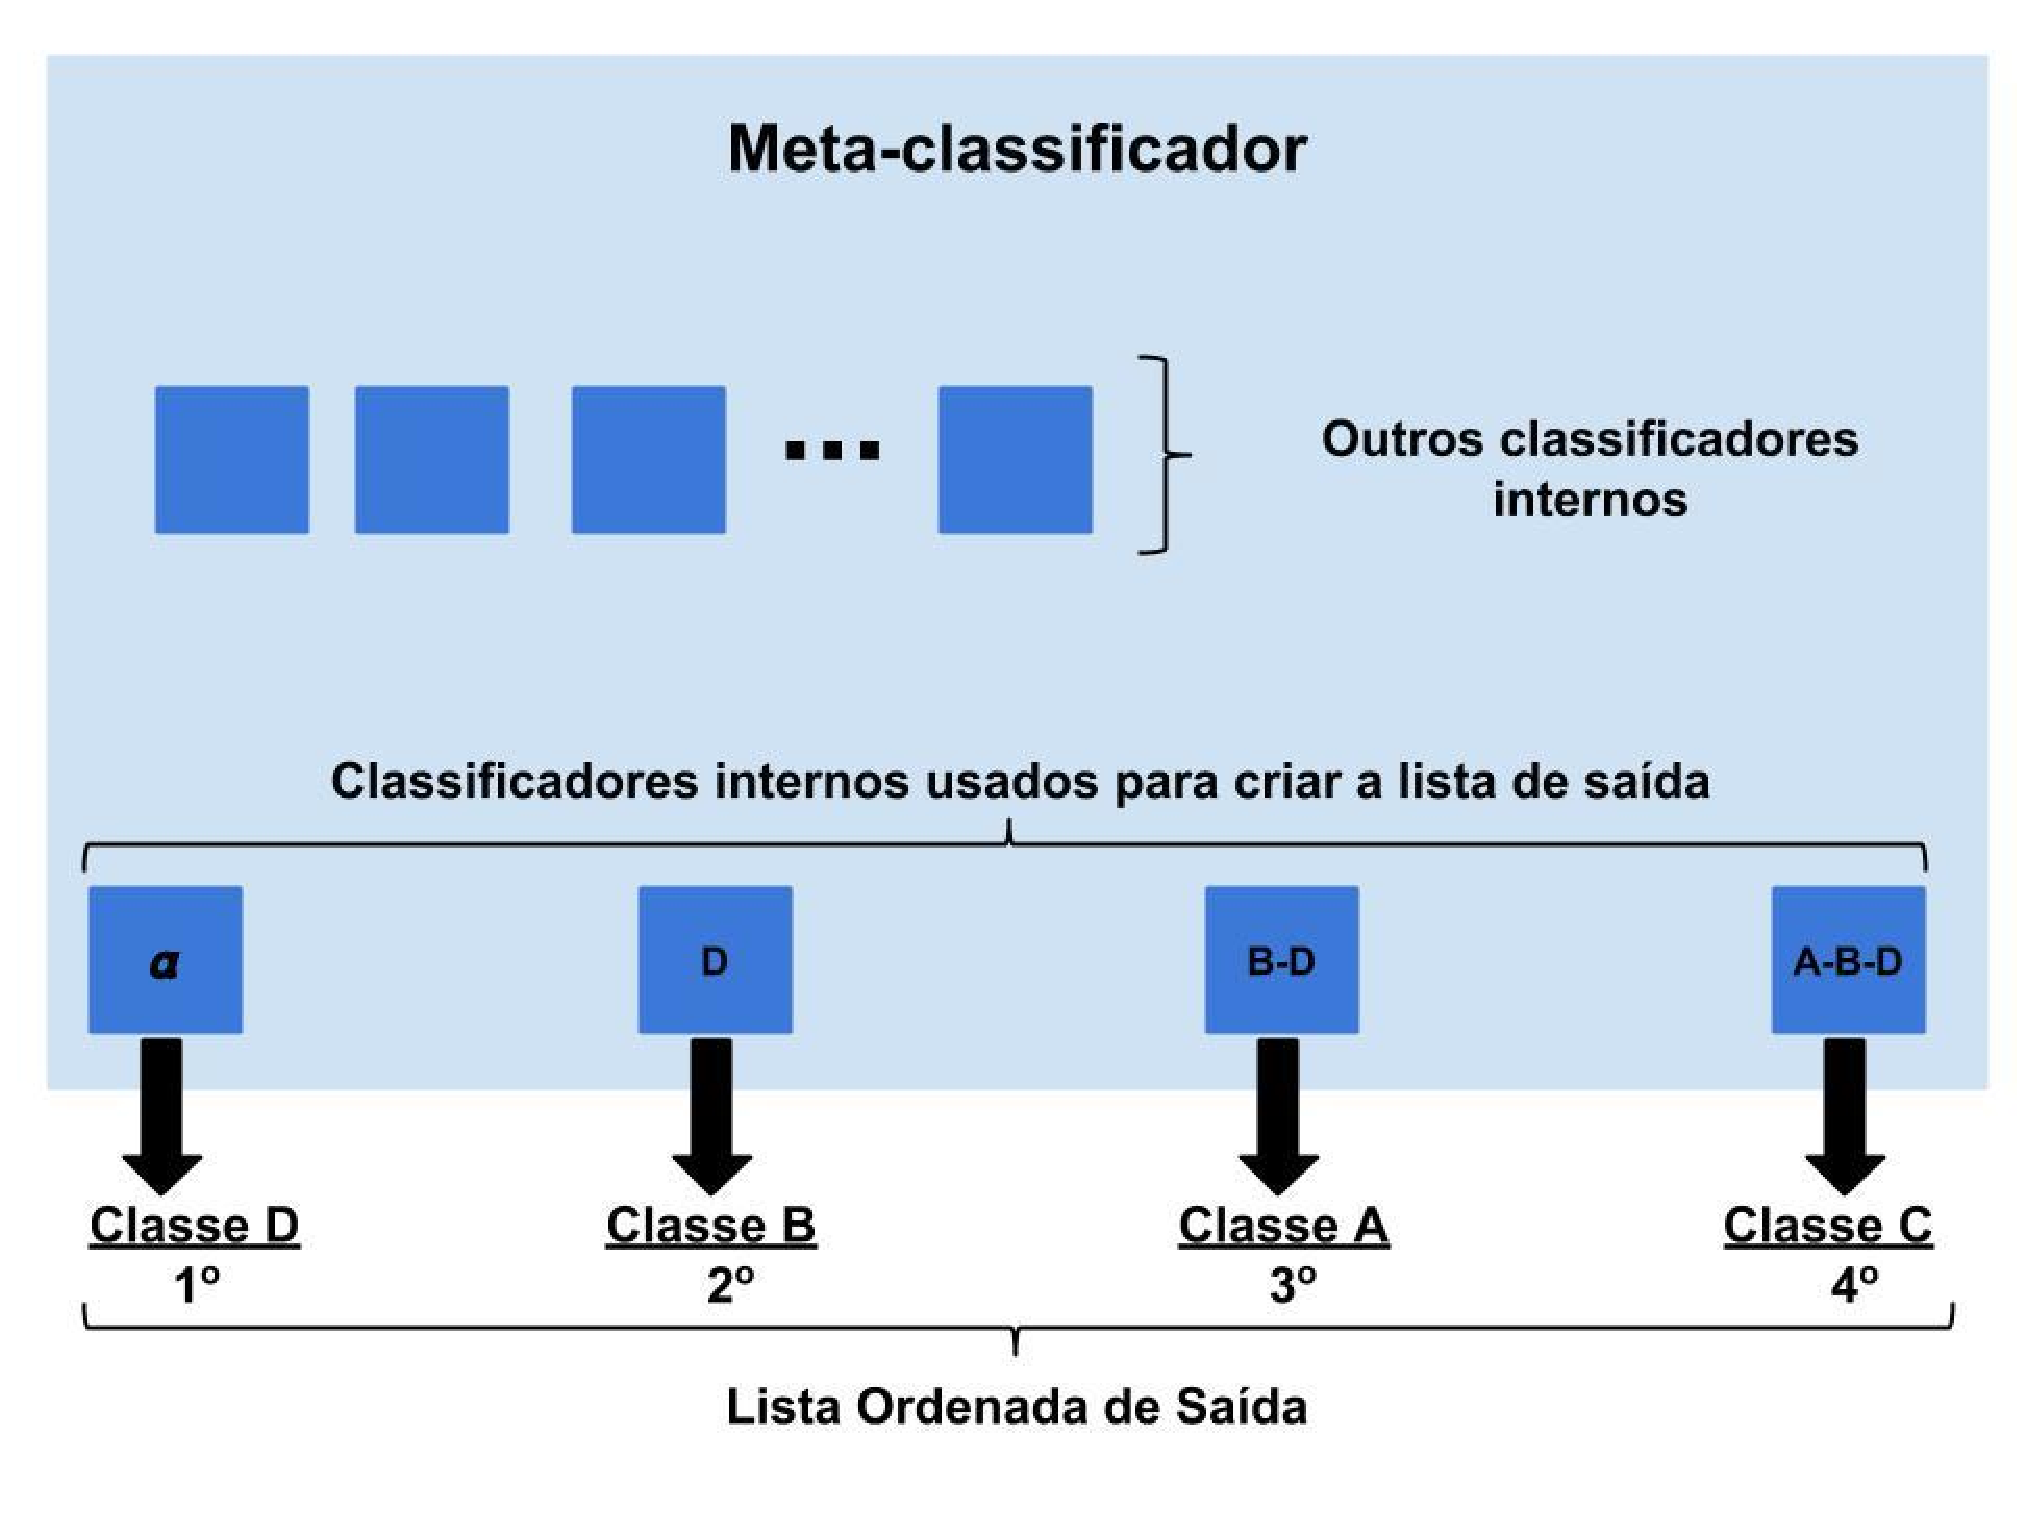
\includegraphics[width=\linewidth]{images/metodoproposto01.eps}
  \caption{Classificadores em cascata e lista de saída.}
  \label{fig:metodoproposto01}
\end{figure}

A Figura \ref{fig:metodoproposto01} ilustra como a lista de saída é gerada pelos classificadores internos.
Assuma que temos 5 classes distintas no conjunto de dados: A, B, C, D e E. 
No exemplo da Figura \ref{fig:metodoproposto01} queremos gerar uma lista de saída de tamanho quatro, logo quatro classificadores internos são utilizados. 
O classificador inicial (alfa),que foi treinado com o conjunto de treino completo, sempre gera o primeiro item de uma lista. 
O metaclassificador precisa então escolher um de seus classificadores internos para gerar um próximo item. 
Como a Figura sugere, esta escolha depende de todos os elementos inseridos anteriormente na lista.
Repare na notação utiliza para nomear os classificadores, as letras depois barra "/" indicam as classes retiradas do conjunto de treino original para treinar aquele classificador.
Ou seja, o classificador /D foi treinado com um conjunto de treino filtrado de forma a excluir todas as instâncias da classe D, já o /BD excluiu aquelas das classes B e D e assim por diante.
Desta forma, o classificador /BD foi usado para gerar o terceiro elemento da lista por que as classes B e D já tinham sido colocadas na mesma.
Com isso o conjunto de treino utilizado para este classificador está livre da influência dessas classes.

\section{Funcionamento do Metaclassificador}

Seja \textit{T} o conjunto de treino do metaclassificador e \textit{v} o número de valores distintos que seu atributo classe pode assumir. 
Este conjunto será filtrado de formas diferentes e então utilizado para treinar os classificadores internos. 
Somente o classificador inicial, usado para gerar o primeiro elemento da lista de saída, é treinado com o conjunto de treino \textit{T} completo. 
Qualquer outro classificador interno é treinado com uma versão filtrada de  \textit{T}. 
De forma geral, o classificador que será usado para classificar o item da lista na posição \textit{k}, onde \textit{k} $<$ \textit{v}, deve ser treinado com um conjunto de treino filtrado \textit{k-1} vezes. 
Estas filtragens retiram sucessivamente do conjunto de treino as instâncias cujas classes já foram colocadas na lista.

No exemplo anterior, da Figura \ref{fig:metodoproposto01}, o classificador /ABD é usado para gerar o quarto elemento da lista.
Este classificador foi treinado com um conjunto filtrado 3 vezes (para retirar as instâncias com as classes A, B e D).
O processo de treinamento e classificação para um classificador interno é ilustrado na Figura \ref{fig:metodoproposto02}.

Note que o metaclassificador não foi desenvolvido para receber um conjunto de treino com uma lista ordenada no gabarito. 
Ele deve ser treinado com conjuntos que apresentam apenas um único valor no atributo classe.
Apos o treinamento com um conjunto de dados deste tipo o metaclassificador é capaz de gerar uma lista ordenada de classes para uma nova instância.

\section{Motivação}
\label{sec:mp_motivacao}

A principal motivação para utilização deste método é a eliminação de ruído dos dados.
Como explicamos na seção anterior isso é feito através de filtragens sucessivas do conjunto de treino que eliminam as instâncias cuja classe já foi colocada na lista.
Para entender melhor a vantagem desta abordagem considere o caso de conjuntos de dados desbalanceados.
Isto é, que tem instâncias de diversas classes diferentes porém uma com a quantidade muito maior do que o restante.

\begin{figure}[h!]
  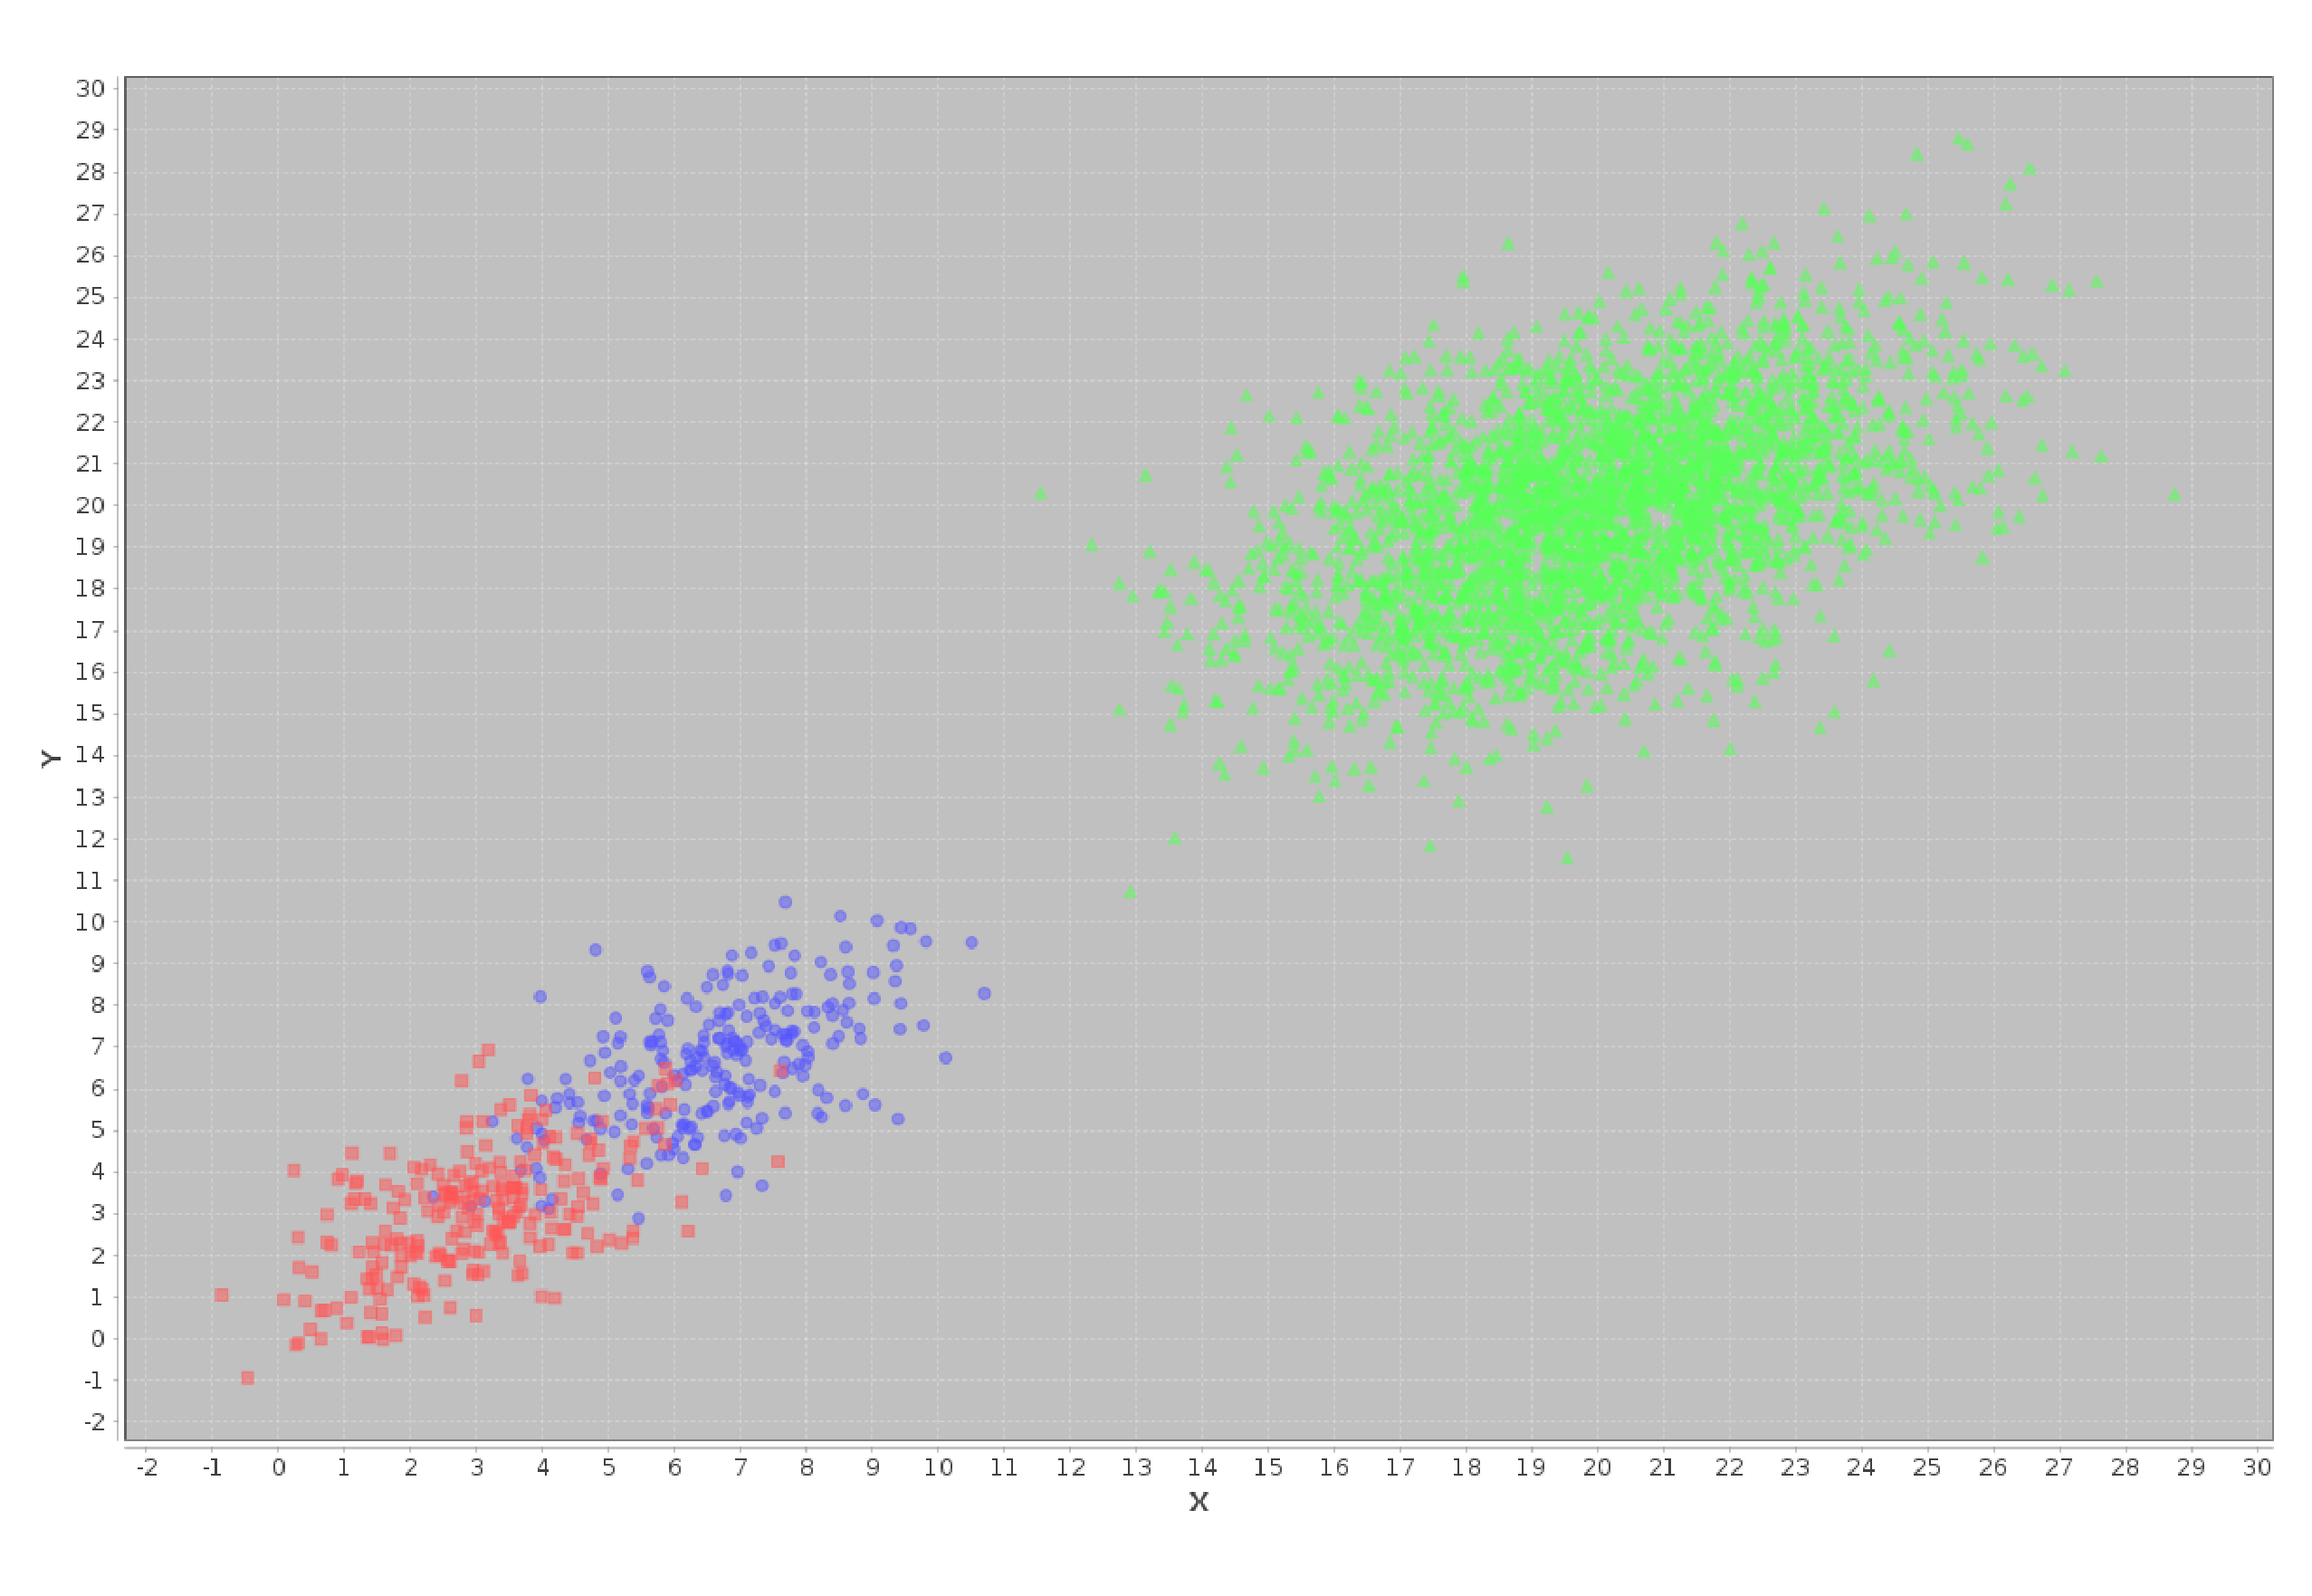
\includegraphics[width=\linewidth]{images/random_data_01.eps}
  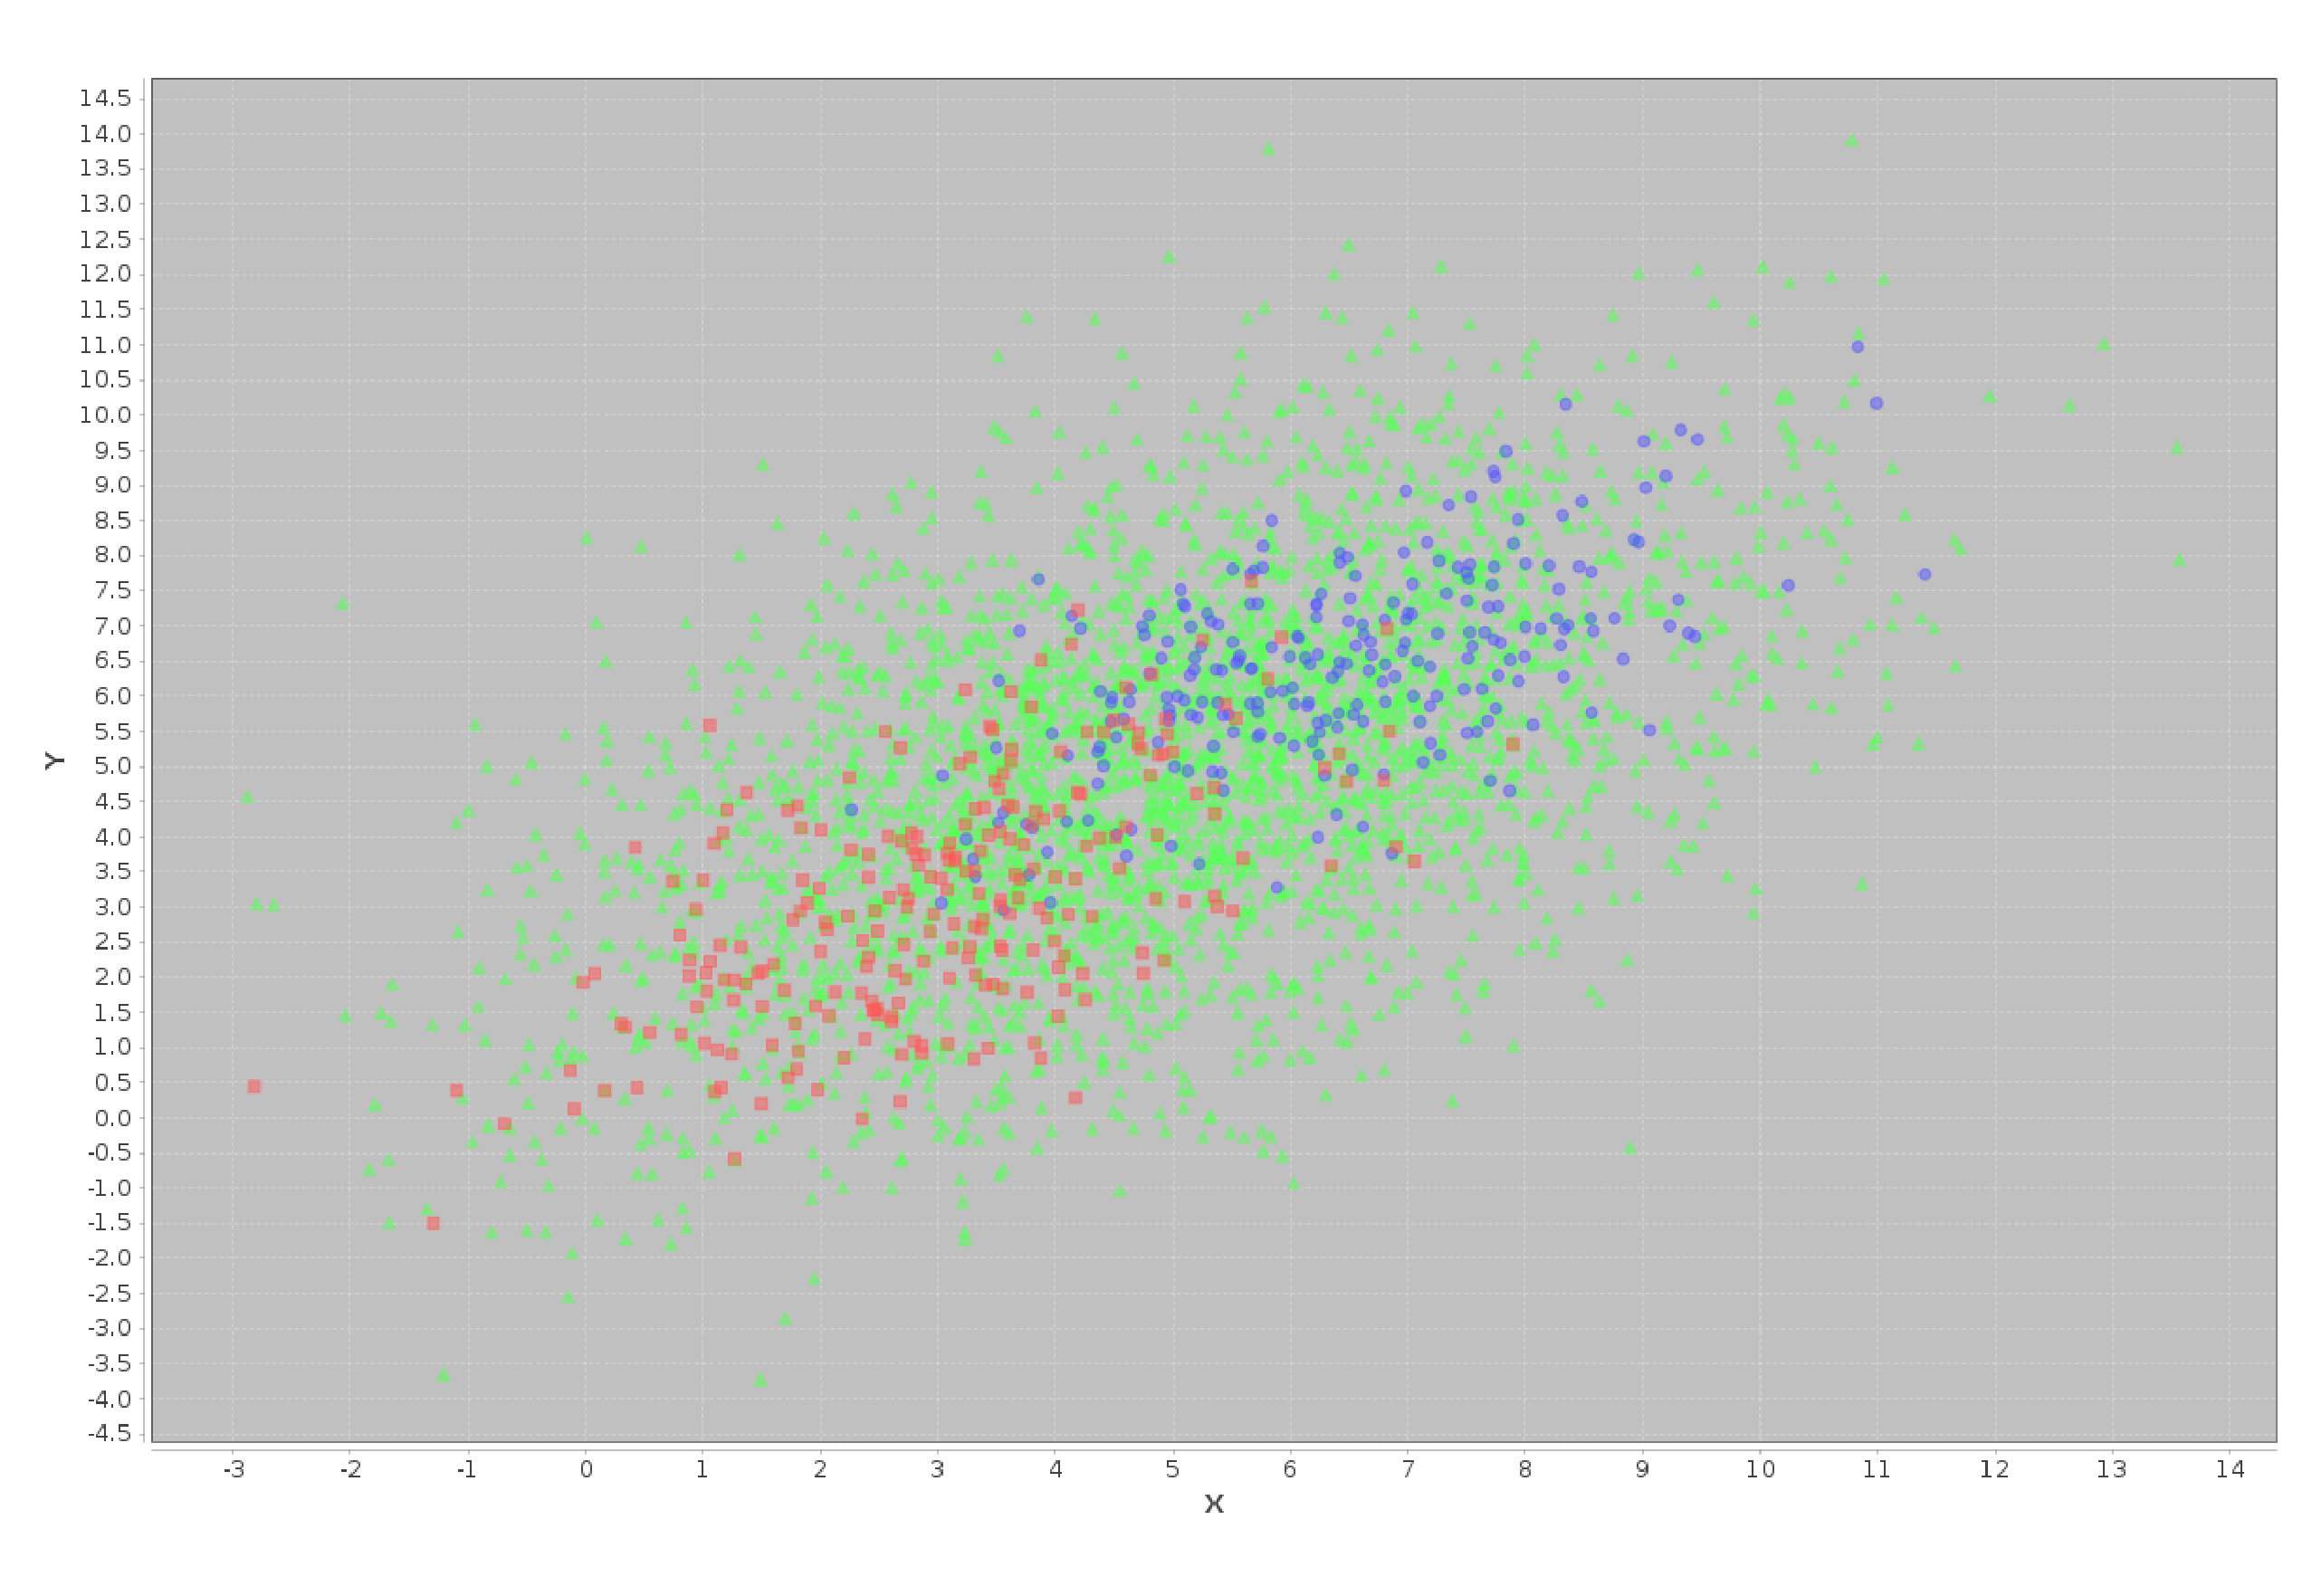
\includegraphics[width=\linewidth]{images/random_data_50.eps}
  \caption{Conjuntos de dados desbalanceados.}
  \label{fig:dadosdesbalanceados}
\end{figure}

A Figura \ref{fig:dadosdesbalanceados} ilustra dois conjuntos de dados desbalanceados gerados aleatoriamente.
Ambos tem a mesma quantidade de pontos, que estão agrupados de forma análoga em três grupos diferentes.
Considere que os pontos pertencentes ao mesmo grupo tem também a mesma classe, denotada pela cor: azul, vermelho ou verde.
Note que os dados são desbalanceados pois a classe verde tem uma quantidade de pontos muito maior do que as outras, são 3000 pontos verdes contra 250 azuis e 250 vermelhos.

Cada grupo de pontos foi gerado seguindo uma distribuição normal bivariada.
Apresentamos sua função densidade de probabilidade para um vetor aleatório \textit{(x,y)} a seguir.

\begin{equation*}
\resizebox{.99\hsize}{!}{
$f(x,y)=\frac{1}{2\pi \sigma _x\sigma _y\sqrt{1-\rho ^2}}\exp \left\{ -\frac 1{2(1-\rho ^2)}\left[ \left( \frac{x-\mu _x}{\sigma _x}\right) ^2-2\rho \left( \frac{x-\mu _x}{\sigma _x}\right) \left(\frac{y-\mu _y}{\sigma _y}\right) +\left( \frac{y-\mu _y}{\sigma _y}\right)^2\right] \right\}$
}
\end{equation*}

onde,

- $\mu$ é o vetor de médias dado por $\[ 
\left( \begin{array}{c}
\mu _x \\
\mu _y
\end{array} 
\right)\] $
 
- $\rho$ é a correlação entre x e y

- $\sigma$ remete à matriz de covariâncias $\Sigma=\[ \left( \begin{array}{cc}
\sigma _x ^2 & \rho \sigma _x \sigma _y \\
\rho \sigma _x \sigma _y & \sigma _y ^2 
\end{array} 
\right)\] $
\end{itemize}
\newline

No primeiro cenário da Figura \ref{fig:dadosdesbalanceados} os dados da distribuição que contem mais pontos (classe verde) estão afastados do restante.
Em contraste, no segundo cenário a média da distribuição de pontos verdes está entre os centros das distribuições de pontos vermelhos e azuis.
Depois de realizar testes com os dois conjuntos de dados percebemos que alguns classificadores, e.g. \textit{k nearest neighbors}, tem acurácias mais elevadas no primeiro cenário.
Notadamente, a presença da grande quantidade de pontos verdes próximos ao restante dificulta o aprendizado do classificador e piora o resultado final.

O método introduzido neste trabalho foi proposto no intuito de melhorar o resultado de casos como esse.
Suponha que queremos montar uma lista ordenada das cores mais prováveis para um ponto.
De acordo com o que já foi apresentado sobre o método, depois de selecionar um ponto verde para a lista, instâncias dessa classe serão eliminadas do conjunto de treino.
Desta forma o classificador utilizado para gerar o próximo elemento será treinado com um conjunto de treino sem a influência da classe mais numerosa (responsável pelo desbalanceamento).
Veremos em mais detalhes no capítulo \ref{chap:descricaodostestes} os resultados obtidos por nossa abordagem.

\section{Versões do método}
\label{sec:versoesdometodo}

O método proposto foi desenvolvido em duas versões: estático e dinâmico.


\subsection{Método Estático}

O método estático gera a priori todas os subconjuntos de classe que podem compor a lista de saída. 
Ele então treina todos os possíveis classificadores, cada um com sua versão filtrada do conjunto de treino, armazenando-os internamente.
Este conjunto de classificadores internos é efetivamente o modelo gerado pelo metaclassificador. 
Este pode ser usado então para gerar rankings ao receber novas instâncias. 

O pseudocódigo a seguir descreve o procedimento de treinamento e classificação para a versão estática do método.
\\

\hline
\begin{center}
\textbf{Pseudocódigo: Funcionamento do Metaclassificador}

\textbf{Versão Estática}
\end{center}
\hline
\hfill \break
-- \textit{Treinamento}\newline
Carrega o conjunto de treino completo\newline
Gera todos os possíveis subconjuntos de classe (de tamanho k ou menor) sem repetições\newline
Para cada combinação de classe que foi gerada faça:

\quad Copia o conjunto de treino completo

\quad Remove da cópia os exemplos dessas classes

\quad Treina um classificador com este conjunto de treino modificado

\quad Armazena internamente o modelo gerado\newline
-- \textit{Classificação}\newline
Para cada item \textit{i} da lista de saída faça:

\quad Verifica as \textit{i-1} classes que já foram colocadas na lista de saída

\quad Recupera o modelo interno treinado sem essas classes

\quad Utiliza este modelo para gerar o \textit{i-ésimo} item da lista de saída

\hline
\hfill \break

Note que, quanto mais valores a classe do conjunto de treino original puder assumir, mais classificadores internos comporão o modelo do metaclassificador.
Sejam \textit{N} o número de classificadores geados pelo método estático, \textit{v} o número de valores de classe distintos no conjunto universo e \textit{k} o tamanho da lista que se deseja gerar. 
De forma geral, considerando que $\textit{k} \leq \textit{v}$, temos que:

\begin{equation*}

\centering
\textit{N} = \sum\limits_{i=0}^k \binom{v}{i}

\end{equation*}

A Figura \ref{fig:metodoproposto03} ilustra os classificadores internos gerados quando as possibilidades de valor de classe são A, B, C e D. Na Figura as numerações não somente identificam cada classificador interno, elas denotam como o conjunto de treino foi filtrado para gerar aquele classificador. Além disso, a Figura divide os classificadores internos em camadas. Um classificador que pertence a camada \textit{k} pode ser usado apenas para gerar um elemento na posição \textit{k} da lista de saída.

\begin{figure}[h!]
  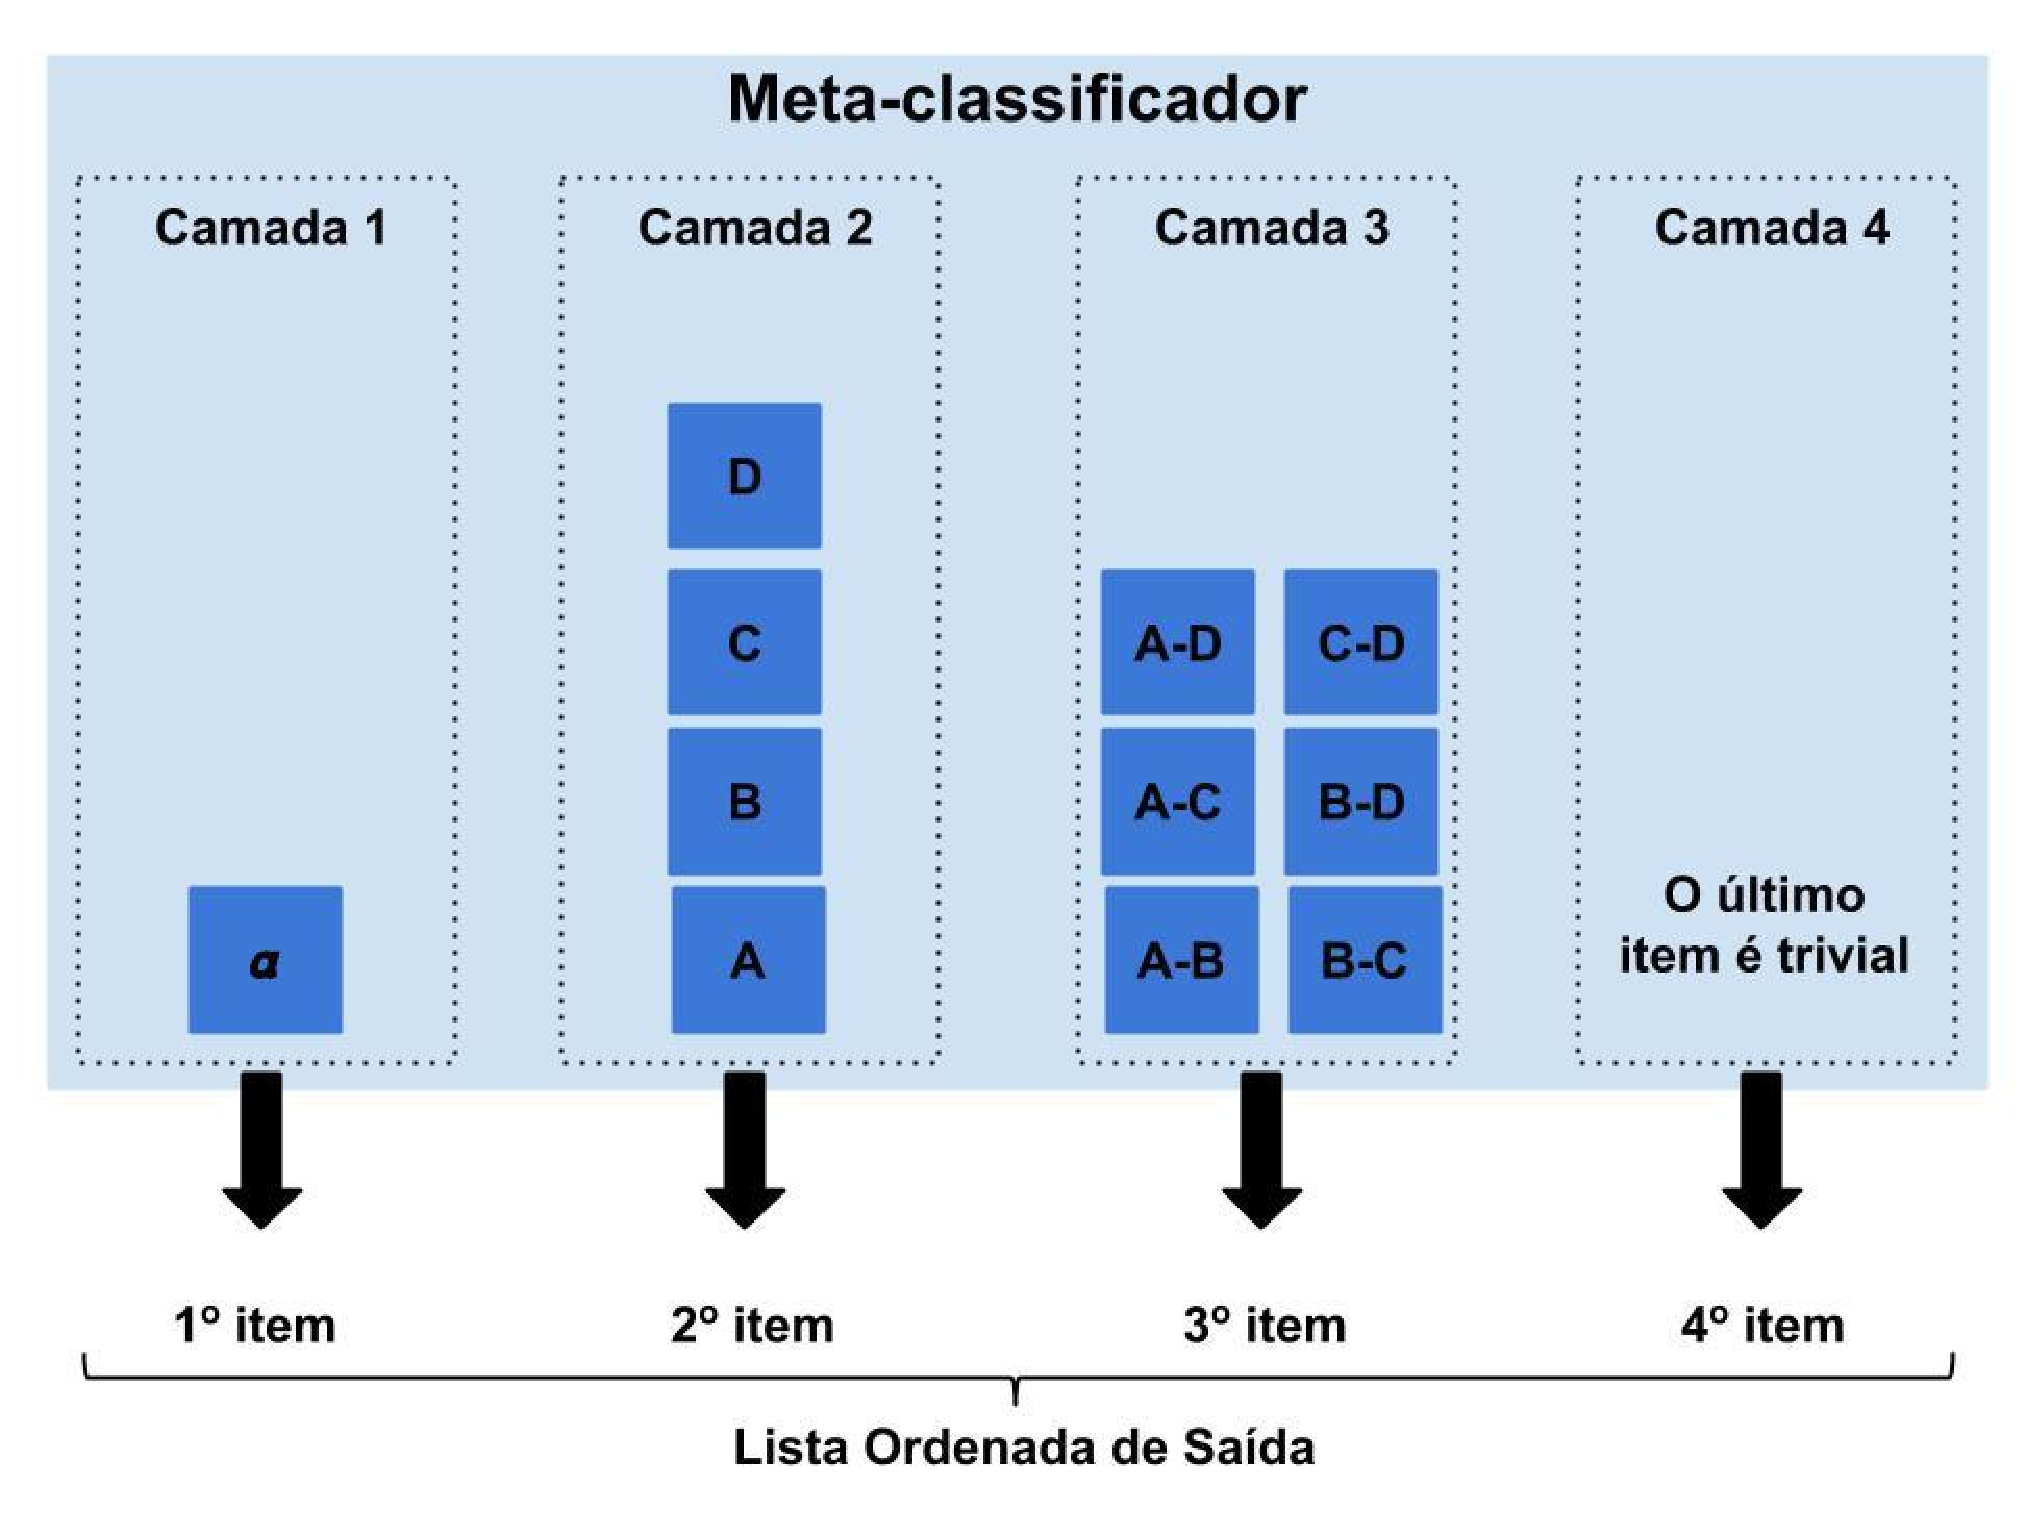
\includegraphics[width=\linewidth]{images/metodoproposto03.eps}
  \caption{Camadas de classificadores internos.}
  \label{fig:metodoproposto03}
\end{figure}

A versão estática pode ser lenta durante a fase de treinamento, pois precisa treinar um grande número de classificadores antes de classificar qualquer nova instância. Por outro lado, uma vez treinado o modelo pode ser usado para classificar diversas novas instâncias rapidamente.

\subsection{Método Dinâmico}

O método dinâmico constrói o modelo na medida do necessário, treinando apenas os classificadores requeridos para a construção da lista de saída para a instância em questão. Ou seja, o modelo é treinado ao mesmo tempo que a classificação de instâncias é feita. De forma análoga ao método anterior, os classificadores são armazenados internamente a medida que são treinados. Desta forma, ao construir a lista de saída, os classificadores já treinados são reutilizados. Sendo assim, um mesmo classificador nunca é treinado mais de uma vez. 

O pseudocódigo a seguir descreve o procedimento de treinamento e classificação para a versão dinâmica do método.
\\

\hline
\begin{center}
\textbf{Pseudocódigo: Treinamento de Classificador Interno}

\textbf{Versão Dinâmica}
\end{center}
\hline
\hfill \break
Carrega o conjunto de treino completo\newline
Para cada item \textit{i} da lista de saída (onde $1 \leq i \geq k$) faça:

\quad Verifica as \textit{i-1} classes que já foram colocadas na lista de saída

\quad Copia o conjunto de treino completo

\quad Remove da cópia os exemplos das \textit{i-1} classes já incluídas na lista

\quad Treina um classificador com o conjunto de treino modificado

\quad Armazena internamente o modelo gerado

\quad Utiliza este modelo para gerar o \textit{i-ésimo} item da lista de saída
\hline
\hfill \break

\begin{figure}[h!]
  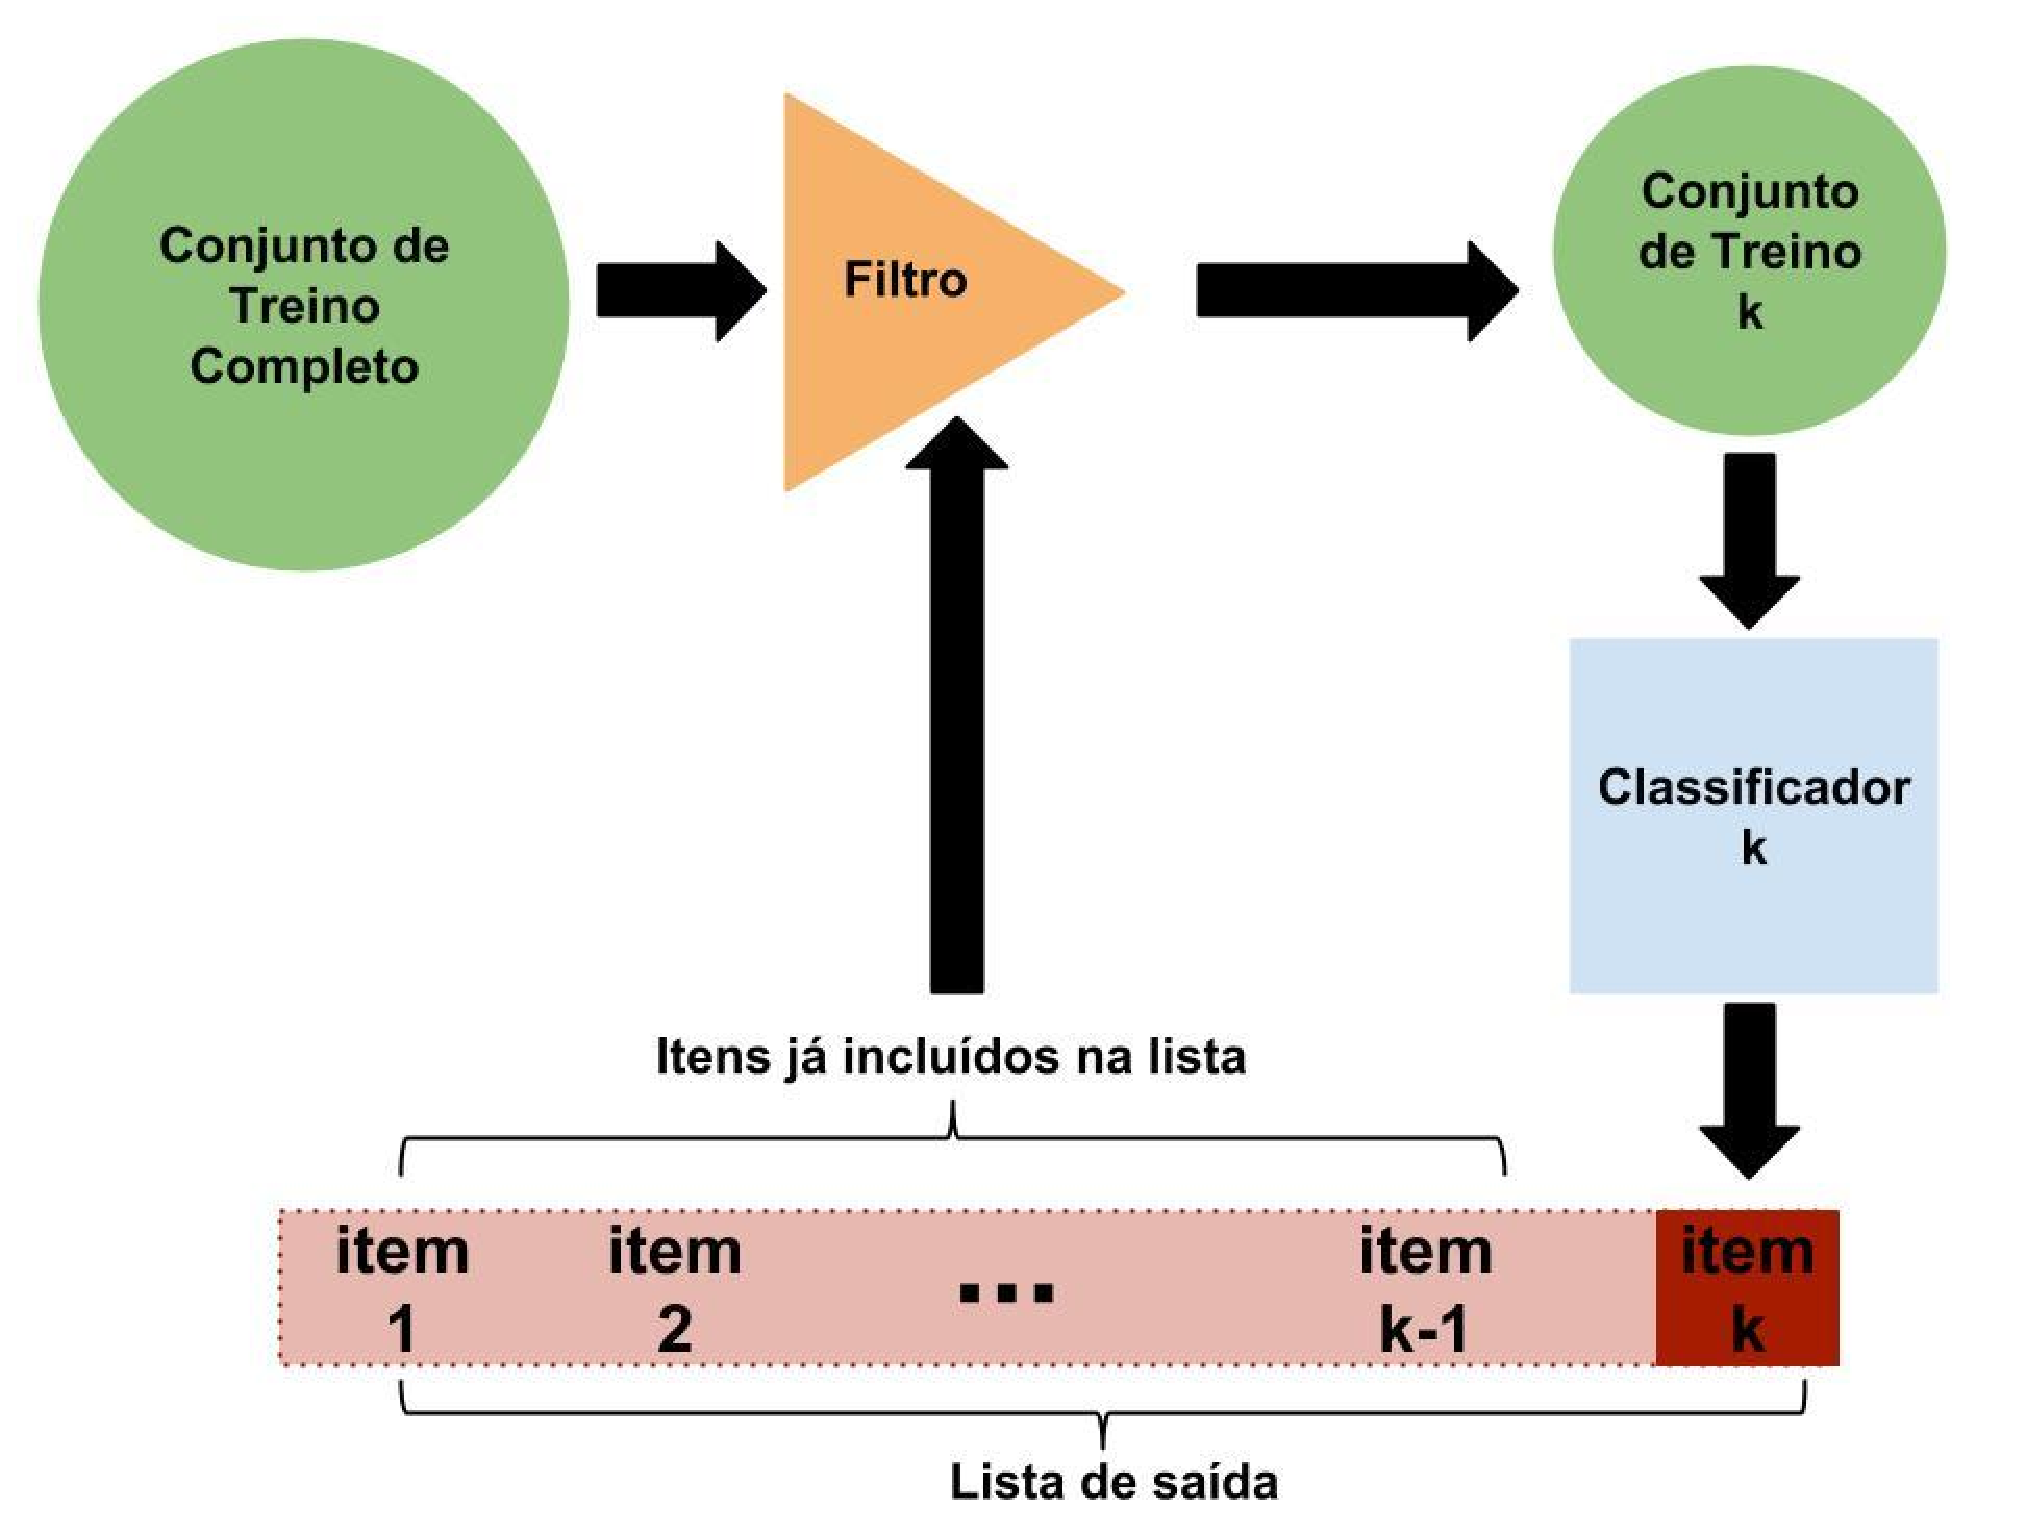
\includegraphics[width=\linewidth]{images/metodoproposto02.eps}
  \caption{Filtragem do conjunto de treino e treinamento de um classificador.}
  \label{fig:metodoproposto02}
\end{figure}

Esta segunda versão tende a ser mais rápida do que a anterior, visto que não precisa treinar todas as possíveis combinações de classificadores a priori. Entretanto, como o treinamento do modelo é feito ao mesmo tempo que a classificação de instâncias, o tempo de classificação da versão dinâmica é maior do que a versão estática. 

Concretamente, sejam \textit{k} o tamanho da lista de saída, \textit{M} o tempo médio de treinamento de um classificador interno e \textit{t} o tempo médio de classificação de um único item por um classificador interno já treinado. Note que tipicamente temos que $ \textit{M} >> \textit{t} $. Considere o caso onde o metaclassificador ainda não tem um classificador interno treinado. Usaremos este como limite superior para o tempo de construção da lista de saída para uma nova instância. Este tempo é calculado por $ \textit{T} = \textit{k}\left(\textit{M} + \textit{t}\rigth) $. Por outro lado, o limite inferior para o tempo \textit{T} ocorre no caso onde o metaclassificador já treinou a priori todos os classificadores internos necessários na construção da lista de saída de uma nova instância. Neste caso temos $ \textit{T} = \textit{k}\textit{t} $.

\section{Vantagens e Desvantagens do método}

O método proposto tem a versatilidade de permitir o uso que qualquer classificador internamente. Além disso, as sucessivas filtragens do conjunto de treino removem as instâncias com classes que não são mais pertinentes para construção da lista de saída. Estas duas características podem contribuir para melhoria do resultado final com (1) a escolha do classificador interno mais adequado e (2) a remoção de ruído do conjunto de treino.

Uma desvantagem deste método é o alto custo computacional do treinamento dos classificadores internos, tanto em processamento quanto em memória. Dependendo da quantidade de valores de classe, o modelo do metaclassificador pode requerer o treinamento de centenas ou milhares de classificadores internos. Esta desvantagem pode vir a ser proibitiva para a versão estática do método. 

A versão dinâmica mitiga este problema pois treina os classificadores internos somente quando são necessários. Desta forma ela economiza processamento em comparação com a versão estática. Ainda assim, pode ser necessário grandes quantidades de memória durante a execução do programa. Com isso podendo ser inviável a execução do mesmo na maioria das máquinas. Portanto, um gerenciamento de memória foi desenvolvido. Este garante que a memória alocada não superará um limiar máximo, especificado no momento da execução do programa.

A solução desenvolvida em Java para implementar o método proposto mantém um conjunto interno de objetos, que são classificadores já treinados. Com o gerenciamento de memória, sempre que a memória alocada pelo programa atingir um determinado patamar \textit{M}, um número \textit{c} de classificadores é removido do conjunto. Estes classificadores são removidos do menos usado para o mais usado. Tanto \textit{M} quanto \textit{c} podem ser ajustados pelo usuário no momento da execução do programa. Note que para que isto funcione \textit{M} deve ser menor do que a quantidade máxima de memória disponível. Desta forma, em um momento posterior a exclusão destes classificadores internos, o \textit{Garbage Collector} do Java liberará a memória. Com isso está garantido que o programa não poderá ficar com memória insuficiente para sua execução.


\chapter{Estudo Experimental}
\label{chap:descricaodostestes}

Neste capítulo discutiremos os testes realizados para avaliar o desempenho do método proposto.
Apresentaremos os conjuntos de dados usados e suas características gerais. 
Os algoritmos utilizados internamente no metaclassificador, assim como os \textit{Benchmark} dos testes também serão mostrados.
Por fim, discutiremos os resultados obtidos ao longo dos diversos testes.

\section{O Framework Weka}

Neste trabalho utilizamos o Framework \textit{Weka} para construir o metaclassificador que implementa nosso método proposto. 
O \textit{Weka} é uma coleção de algoritmos de aprendizado para tarefas gerais de mineração de dados \cite{Hall}.
Ele contém ferramentas de preprocessamento, classificação, regressão, clusterização, etc.
Ele pode ser utilizado para aplicar os algoritmos aos dados por meio de sua interface gráfica ou pode ser chamado diretamente de um código Java.

\section{\textit{Benchmark} dos testes}

Para avaliar a performance do método proposto um \textit{benchmark} específico é empregado em cada teste.
Quando um algoritmo é utilizado internamente no metaclassificador, e.g. Árvore de Decisão, o resultado deste mesmo algoritmo sem o metaclassificador é usado como \textit{benchmark}.
Isso é possível pois as classes que implementam estes algoritmos, que fazem parte do \textit{framework} Weka, são capazes de gerar uma distribuição de probabilidades de classes como saída.
A lista de saída que servirá como \textit{benchmark} do teste é então montada a partir desta distribuição de probabilidades.
Isto é, as classes são colocadas na lista na ordem decrescente de probabilidade.
Por exemplo, caso tenhamos as classes A, B, C e D com probabilidades 0.2, 0.25, 0.1 e 0.45 respectivamente, a lista de saída será D, B, A e C.

\section{As métricas de \textit{k-Acurácia}}

Recorde o caso da rede \textit{R} com \textit{n} nodos que podem apresentar falhas.
Imagine que sempre que a rede apresenta uma falha precisamos enviar uma ou mais equipes à nodos diferentes no intuito de corrigir o problema rapidamente.
No pior caso, sem qualquer indicio de onde a falha ocorreu, enviaremos \textit{n} equipes.
Porém, se por exemplo estivermos na dúvida entre apenas três nodos, saberemos que somente três equipes serão necessárias.

As métricas apresentadas nessa seção foram desenvolvidas para avaliar a performance dos modelos de acordo com esse cenário.
No caso da rede, precisamos de métricas que indiquem o grau de confiança que podemos ter ao enviar um certo número de equipes.
Como foi discutido, o metaclassificador recebe uma instância como entrada, neste caso medições sobre o estado de \textit{R} com ocorrência de falha.
Ele então retorna uma lista ordenada com as \textit{k} classes (nodos) mais prováveis.
De acordo com o problema proposto, a posição da classe verdadeira (nodo com falha) nesta lista é o fator mais importante.
Isto é, se a classe verdadeira aparece em uma das três primeiras posições da lista, este é o caso onde precisamos de apenas três equipes para efetuar o reparo.

Desta forma, a \textit{k-Acurácia} é na verdade um conjunto de métricas.
Elas variam de 1 até \textit{k}; i.e. \textit{1-Acurácia}, \textit{2-Acurácia} até \textit{k-Acurácia}; onde \textit{k} denota o tamanho da lista retornada.
Os valores das acurácias para uma dada instância dependem da posição da classe verdadeira na lista.
Se ela está na posição \textit{i}, onde $1 \leq \textit{i} \leq \textit{k}$, então as acurácias anteriores à \textit{i} tem o valor zero e o restante o valor um.
Com isso, a \textit{i-Acurácia} indica a certeza da classe verdadeira aparecer na lista até a posição \textit{i}.
Ou, sob a ótica do problema da rede, a confiança em reparar a falha se enviarmos esse mesmo número de equipes.

Observe na Figura \ref{fig:descricaodostestes01} diversos exemplos de listas e suas acurácias.
Para estes exemplos imagine que temos um conjunto de dados com cinco classes diferentes: A, B, C, D e E.
Considere também que a classe verdadeira em todos os casos ilustrados na Figura é A (em vermelho).
Cada linha do exemplo refere-se então a lista retornada para uma instância distinta e suas consequentes acurácias.

\begin{figure}[h!]
  \centering
  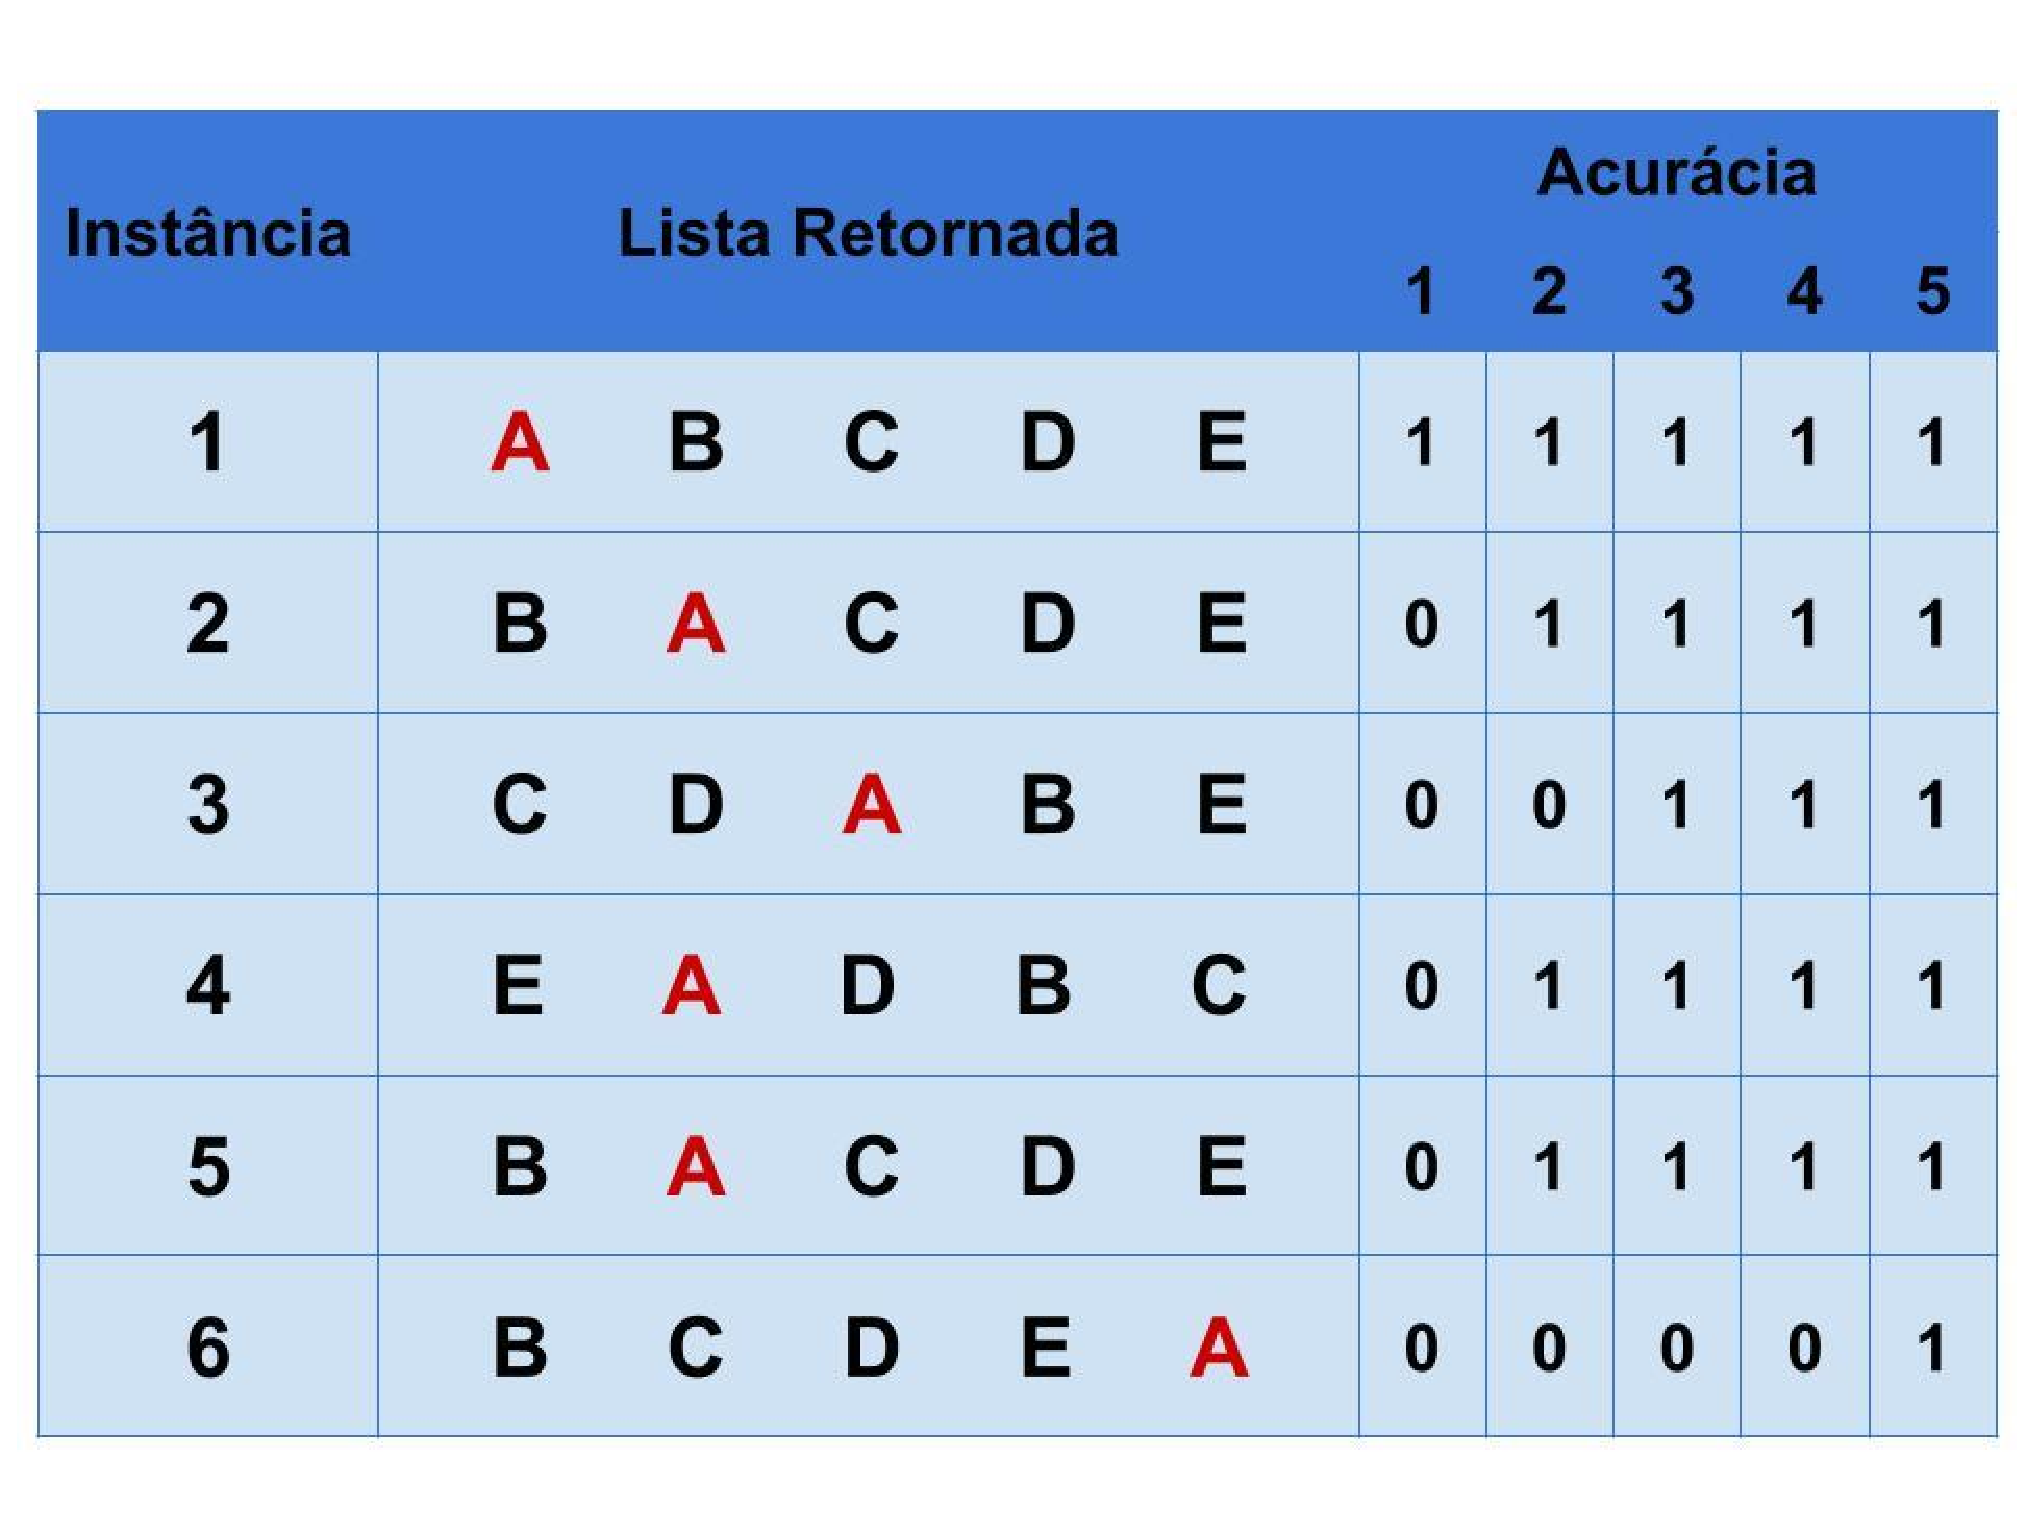
\includegraphics[width=100mm,scale=0.7]{images/descricaodostestes01.eps}
  \caption{Exemplos de listas e suas acurácias.}
  \label{fig:descricaodostestes01}
\end{figure}

Existe ainda uma diferença no cálculo da \textit{k-Acurácia} para o \textit{benchmark} dos testes.
Como a lista de \textit{benchmark} é construída a partir de uma distribuição de probabilidades, podem ocorrer empates.
Quando a probabilidade da classe verdadeira está empatada com a de uma ou mais classes, múltiplas listas poderiam ser criadas a partir desta distribuição.
Considere o caso onde temos as classes A, B e C com probabilidades 0.4, 0.4 e 0.2 respectivamente e a classe verdadeira é A.
Com essas probabilidades podemos ter as listas de saída (1) A, B e C ou (2) B, A e C.
No primeiro caso temos as acurácias de um a três iguais a um.
No segundo caso temos a \textit{1-Acurácia} igual a zero e o restante igual a um.
Entretanto, por ter acesso às probabilidades, a métrica divide os valores.
Teremos então \textit{1-Acurácia} igual 0.5, \textit{2-Acurácia} igual a 1 e \textit{3-Acurácia} igual a 1.

Note que todos os cálculos citados até agora são feitos por instância. 
Ao gerar listas de saída para múltiplas instâncias, os valores obtidos para cada acurácia são somados, formando um valor total por \textit{i-Acurácia}.
Este valor total é então dividido pelo número de instâncias que foram ranqueadas e multiplicado por cem.
Com isso os valores das acurácias apresentados neste trabalho estão na forma de percentuais.

Desta forma, podemos calcular os valores percentuais das acurácias ao longo de todos os exemplos da Figura \ref{fig:descricaodostestes01}.
Os valores são apresentados na tabela \ref{tab:valoresacuraciasexemplo}.

\begin{table}[h!]
  \begin{center}
    \begin{tabular}{cc}
      \hline
      \textbf{Acurácia} & \textbf{Valor Percentual} \\
      \hline

      1 & 16,67 \% \\
      2 & 66,67 \% \\
      3 & 83,33 \% \\
      4 & 83,33 \% \\
      5 & 100 \% \\

      \hline
    \end{tabular}
    \caption{Valores percentuais das acurácias do exemplo}
    \label{tab:valoresacuraciasexemplo}
  \end{center}
\end{table}

\section{As métricas k-Precision e k-Recall}

O \textit{k-Precision} e o \textit{k-Recall} são outros conjuntos de métricas que utilizamos na avaliação do método.
Estes são inspirados nas métricas \textit{Precision} e \textit{Recall}, largamente utilizadas em aprendizado de máquina.
Porém, da mesma forma como fizemos com as \textit{k-Acurácias}, adaptamos essas métricas para avaliar listas de classes de acordo com a posição da classe verdadeira.
Portanto, o \textit{k-Precision} e o \textit{k-Recall} também variam de 1 até \textit{k}; i.e. \textit{1-Precision}, \textit{2-Precision} até \textit{k-Precision}; onde \textit{k} denota o tamanho da lista retornada.

Como sabemos, os valores dessas métricas são calculados a partir da contabilização dos \textit{true positives (tp)}, \textit{false positives (fp)} e \textit{false negatives (fn)} (vide Capítulo \ref{chap:conceitosbasicos}).
Estes por sua vez dependem da posição da classe verdadeira na lista.
Se A é a classe verdadeira e ela aparece na posição \textit{i} da lista, onde $1 \leq \textit{i} \leq \textit{k}$, então as posições anteriores à \textit{i} contam como $fn_A$ e restante como $tp_A$.
Além disso, para cada posição anterior à \textit{i} também é contado um fp para a classe que foi prevista erradamente no lugar de A.

Observe na Figura \ref{fig:descricaodostestes02} o mesmo exemplo anterior agora com a contagem de tp, fn e fp para cada classe.
Recorde que no exemplo temos um conjunto de dados com as classes A, B, C, D e E, sendo A (em vermelho) a classe verdadeira em todos os exemplos.

\begin{figure}[h!]
  \centering
  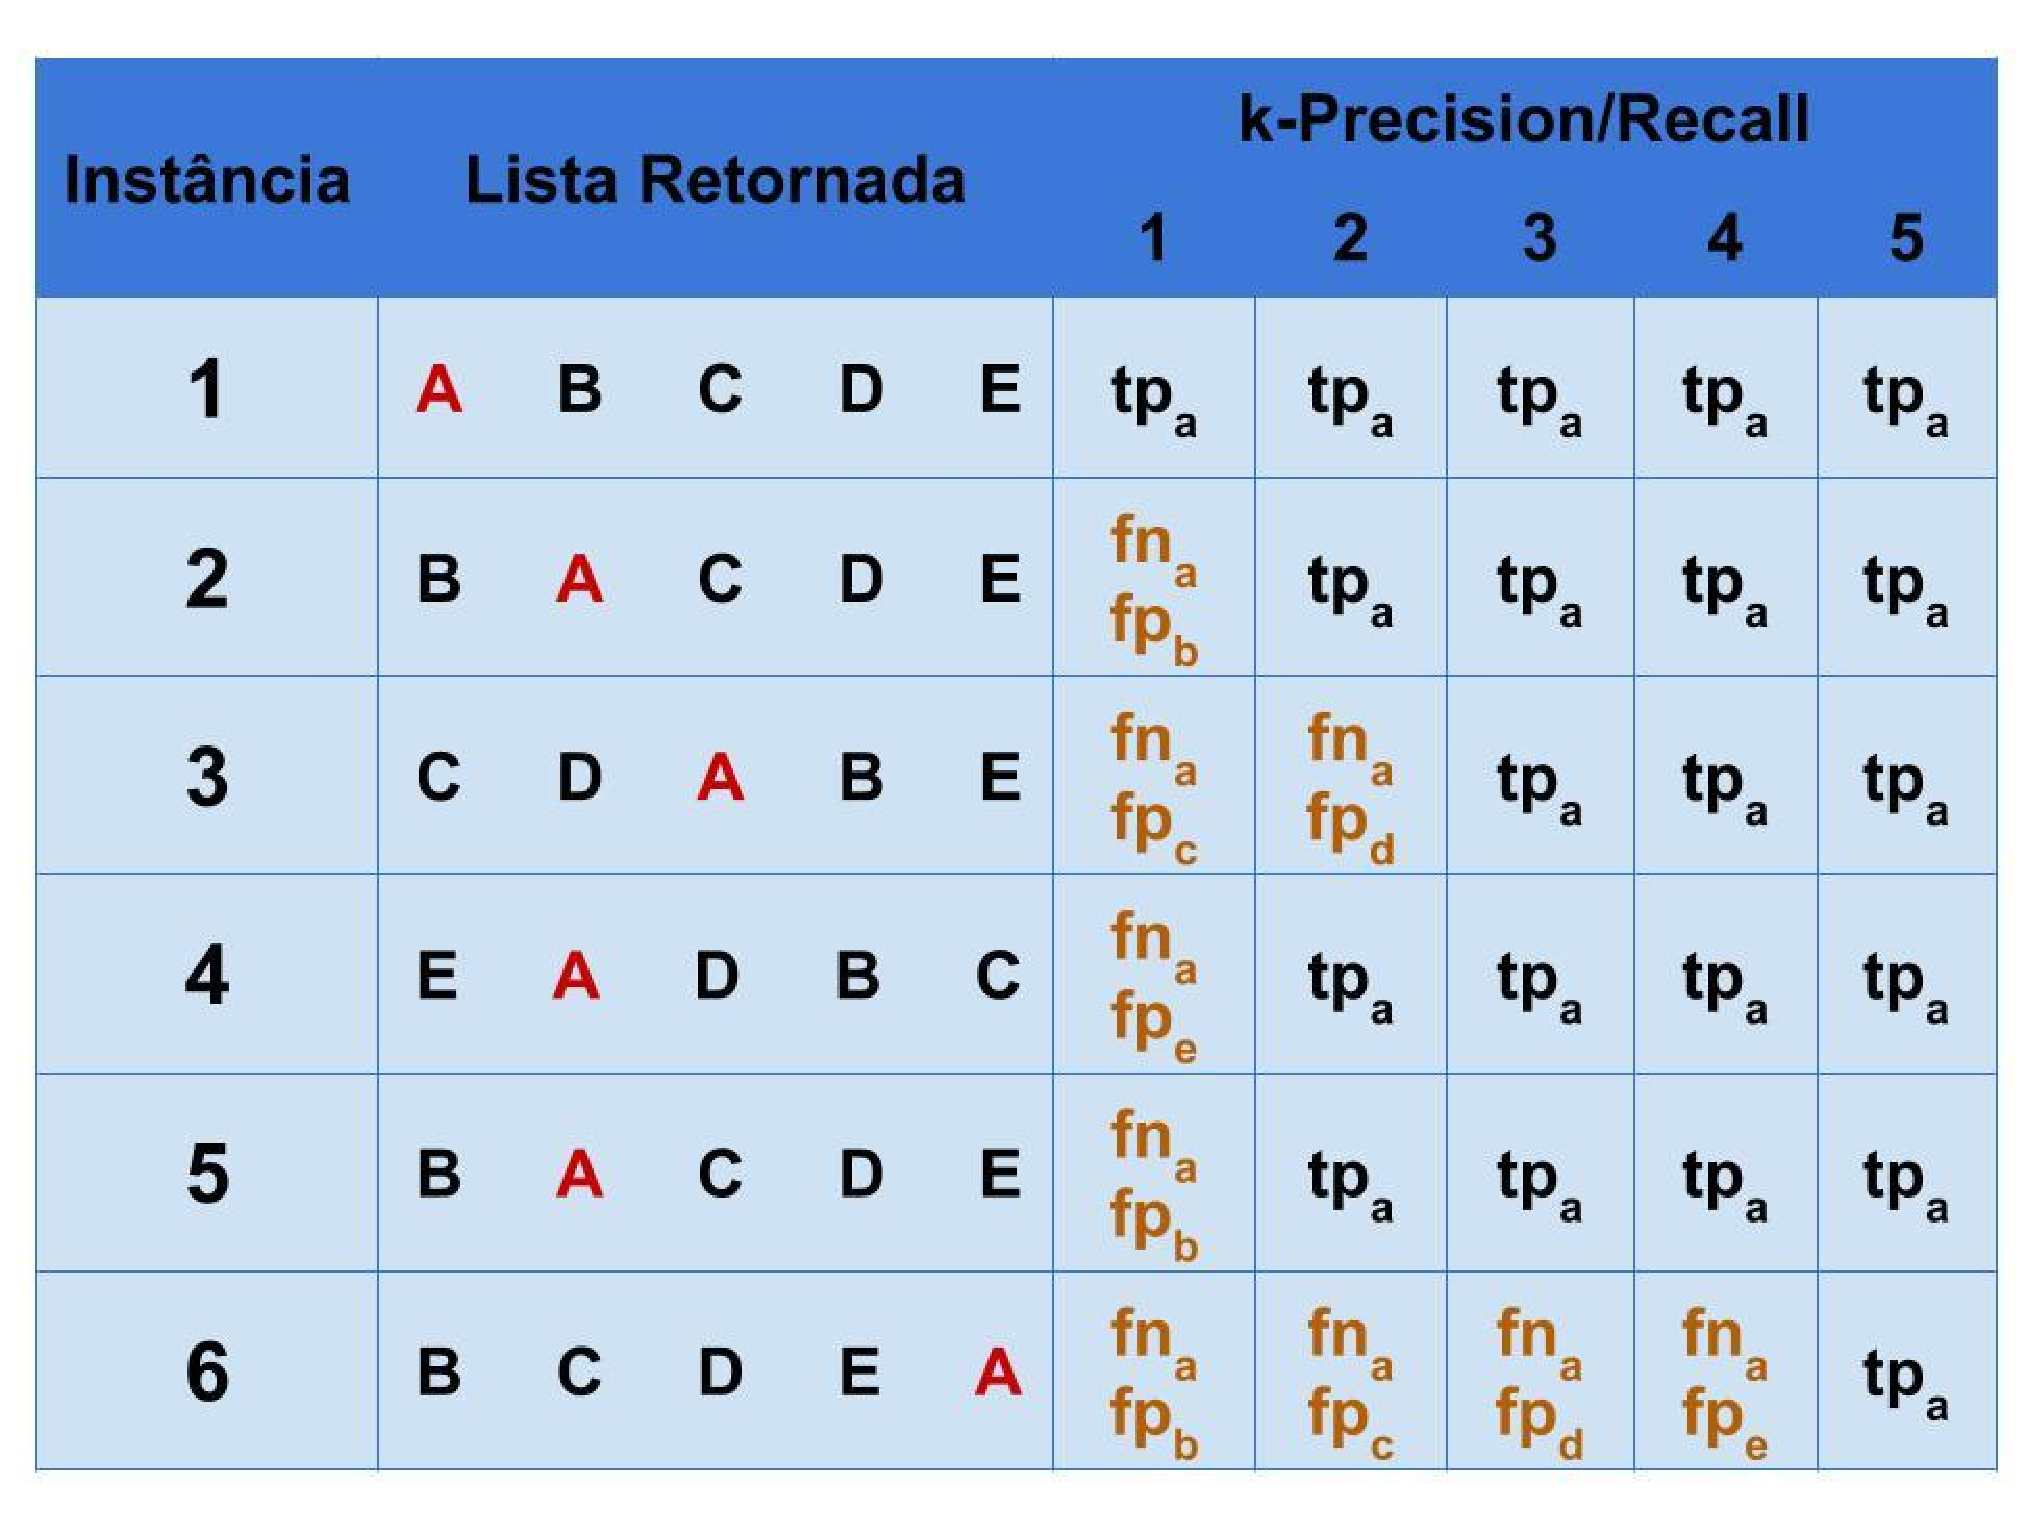
\includegraphics[width=120mm,scale=0.8]{images/descricaodostestes02.eps}
  \caption{Exemplos de listas e suas contagens de tp, fn e fp.}
  \label{fig:descricaodostestes02}
\end{figure}

Da mesma forma que fizemos para as \textit{k-Acurácias} o cálculo é feito de forma diferente para o \textit{benchmark} dos testes.
Lembre que quando a probabilidade da classe verdadeira está empatada com a de uma ou mais classes, múltiplas listas poderiam ser criadas a partir desta distribuição.
Retornemos ao exemplo da seção anterior, onde tínhamos as classes A, B e C com probabilidades 0.4, 0.4 e 0.2 respectivamente e onde a classe verdadeira é A.
Podemos ter as listas de saída (1) A, B e C ou (2) B, A e C.
No primeiro caso as posições de um a três contam como um $tp_A$.
No segundo caso a primeira posição conta um $fn_A$, um $fp_B$ e o restante das posições conta um $tp_A$.
Usando as probabilidades podemos contar de outra forma.
A primeira posição conta 0.5 $tp_A$, 0.5 $fn_A$ e 0.5 $fp_B$, visto que existe 50\% de chance de cada caso ocorrer.
O restante das posições conta simplesmente como um $tp_A$.

O cálculo do \textit{k-Precision} e do \textit{k-Recall} é feito de duas formas: \textit{Micro} e \textit{Média Ponderada}.
No primeiro caso somamos os \textit{true positives (tp)}, \textit{false positives (fp)} e \textit{false negatives (fn)} de todas as classes para cada \textit{i-Precision} e \textit{i-Recall}.
Depois aplicamos esses valores totais às fórmulas do \textit{Precision} e \textit{Recall}.
No segundo caso calculamos as métricas, usando as fórmulas, para cada classe a priori.
Depois tiramos uma média ponderada pela quantidade de cada classe no conjunto de dados.
Em ambos os casos os valores apresentados neste trabalho são convertidos para a forma de percentuais.

Desta forma, podemos calcular os valores percentuais do \textit{Micro Precision} e \textit{Micro Recall} ao longo de todos os exemplos da Figura \ref{fig:descricaodostestes02}.
Os valores são apresentados na tabela \ref{tab:valores_micro}.
Note que sempre teremos o mesmo valor para essas duas métricas pois a contagem total de \textit{false positives} e sempre igual a de \textit{false negatives}.

\begin{table}[h!]
  \begin{center}
    \begin{tabular}{ccc}
      \hline
      \textbf{k} & \textbf{Precision} & \textbf{Recall} \\
      \hline

      1 & 16,67 \% & 16,67 \% \\
      2 & 66,67 \% & 66,67 \% \\
      3 & 83,33 \% & 83,33 \% \\
      4 & 83,33 \% & 83,33 \% \\
      5 & 100 \% & 100 \% \\

      \hline
    \end{tabular}
    \caption{Valores percentuais do \textit{Micro Precision} e \textit{Micro Recall} do exemplo}
    \label{tab:valores_micro}
  \end{center}
\end{table}

\begin{figure}[h!]
  \centering
  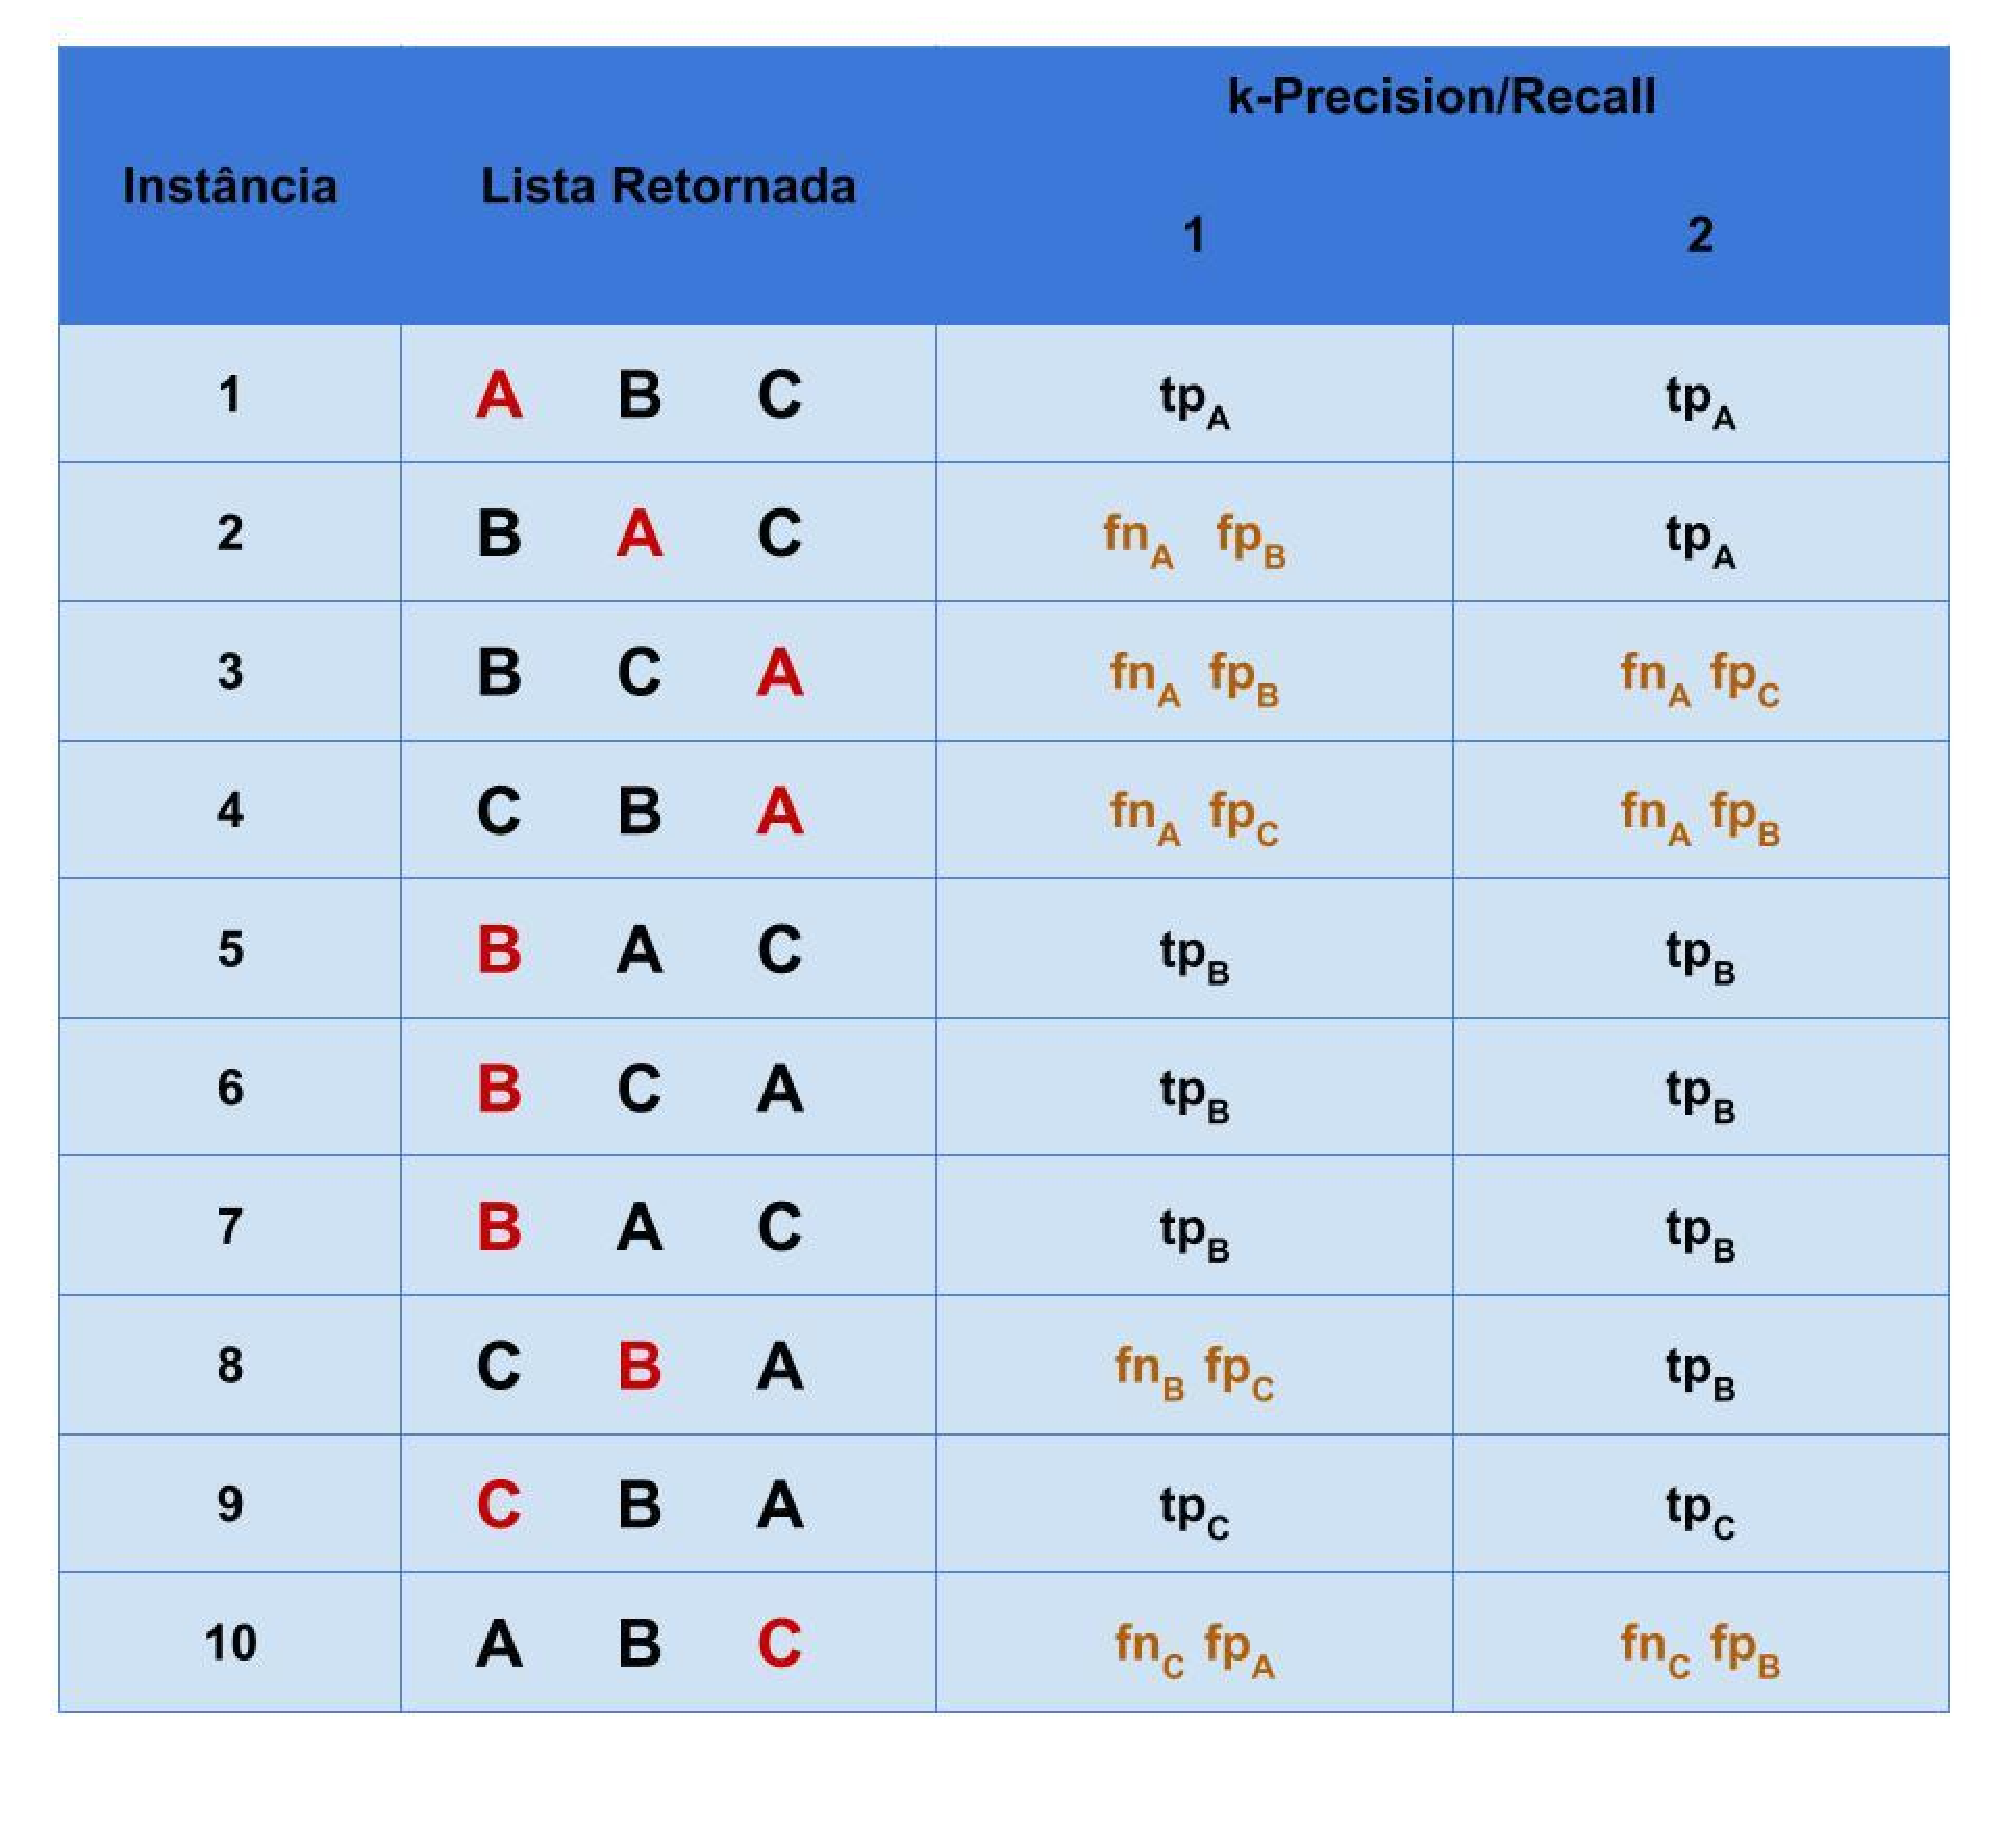
\includegraphics[width=120mm,scale=0.9]{images/descricaodostestes03.eps}
  \caption{Exemplos de listas com três classes e suas contagens de tp, fn e fp.}
  \label{fig:descricaodostestes03}
\end{figure}

Para entender o cálculo do \textit{Precision Ponderado} e do \textit{Recall Ponderado} mutilasse, considere outro exemplo onde temos apenas as classes A, B e C.
Este exemplo é apresentado na Figura \ref{fig:descricaodostestes03}, que mostra as dez listas retornadas e suas contagem de \textit{true positives}, \textit{false positives} e \textit{false negatives} para os níveis 1 e 2.

A partir disso podemos chegar às matrizes apresentadas na Tabela \ref{tab:confusao1} para as métricas de nível 1 e \ref{tab:confusao2} para as de nível 2.
Com os valores contabilizados em cada matriz é possível então calcular as métricas de nível 1 e 2 para cada classe, cujos resultados são apresentados na Tabela \ref{tab:valores_classes}.
Por fim, o valor final das métricas ponderadas é apresentado na Tabela \ref{tab:valores_pon}.

Para fazer esses cálculos utilizamos as fórmulas de \textit{Precision} e \textit{Recall} introduzidas no Capítulo \ref{chap:conceitosbasicos}.
Por exemplo, para chegar os valores do \textit{1-Precision Ponderado} da Tabela \ref{tab:valores_pon} devemos fazer os cálculos a seguir.
Considere que $N_A$, $N_B$ e $N_C$ são as quantidades de instancias das classes A, B e C respectivamente.

\begin{align*}
\text{1-Precision Ponderado} &= \frac{(\text{1-$Prec_A$} \times N_A)+(\text{1-$Prec_B$} \times N_B)+(\text{1-$Prec_C$} \times N_C)}{N_A+N_B+N_C} \\
&= \frac{(50\% \times 4)+(60\% \times 4)+(33,33\% \times 2)}{10} \\
&= 50,07\%
\end{align*}

\begin{table}[h!]
  \begin{center}
    \begin{tabular}{cccc}
      \hline
         & \textbf{Real: A} & \textbf{Real: B} & \textbf{Real: C} \\
      \hline

      Previsto: A & 1 & 0 & 1\\
      Previsto: B & 2 & 3 & 0\\
      Previsto: C & 1 & 1 & 1\\

      \hline
    \end{tabular}
    \caption{Contabilização dos valores para métricas ponderadas de nível 1}
    \label{tab:confusao1}
  \end{center}
\end{table}

\begin{table}[h!]
  \begin{center}
    \begin{tabular}{cccc}
      \hline
         & \textbf{Real: A} & \textbf{Real: B} & \textbf{Real: C} \\
      \hline

      Previsto: A & 2 & 0 & 0\\
      Previsto: B & 1 & 4 & 1\\
      Previsto: C & 1 & 0 & 1\\

      \hline
    \end{tabular}
    \caption{Contabilização dos valores para métricas ponderadas de nível 1}
    \label{tab:confusao2}
  \end{center}
\end{table}

\begin{table}[h!]
  \begin{center}
    \begin{tabular}{cccc}
      \hline
       Métrica  & \textbf{Classe A} & \textbf{Classe B} & \textbf{Classe C} \\
      \hline

      \textbf{1-Precision} & 50\% & 60\% & 33,33\% \\
      \textbf{2-Precision} & 100\% & 66,67\% & 50\% \\
      \textbf{1-Recall} & 25\% & 75\% & 50\% \\
      \textbf{2-Recall} & 50\% & 100\% & 50\% \\
      
      \hline
    \end{tabular}
    \caption{Contabilização dos valores métricas ponderadas de nível 1}
    \label{tab:valores_classes}
  \end{center}
\end{table}

\begin{table}[h!]
  \begin{center}
    \begin{tabular}{ccc}
      \hline
      \textbf{k} & \textbf{Precision} & \textbf{Recall} \\
      \hline

      1 & 50,07 \% & 50 \% \\
      2 & 76,67 \% & 70 \% \\

      \hline
    \end{tabular}
    \caption{Valores percentuais do \textit{Precision Ponderado} e \textit{Recall Ponderado} do exemplo}
    \label{tab:valores_pon}
  \end{center}
\end{table}

\section{Resultados dos Testes}

Todos os testes realizados neste capítulo foram realizados com validação cruzada com partição em dez grupos.
Novamente, os componentes do \textit{framework} Weka foram utilizados para realizar as validações.
Além disso, ao executar o programa 10 GB de memória são reservados para o \textit{heap} da Máquina Virtual Java com o comando \textit{java -Xmx10g}.

Todos os testes foram executados em máquinas virtuais no ambiente \textit{Google Cloud Platform}. 
Estas máquinas tinham a seguinte configuração: sistema operacional Linux Ubuntu 14.04, duas unidades de processamento (vCPU) e 13 GB de memória RAM.

Na Tabela \ref{tab:algoritmostestes} são apresentadas as configurações de algoritmos usados nos testes. Todas as classes utilizadas são do pacote \textit{weka.classifiers}.

\begin{table}[h!]
  \begin{center}
    \begin{tabular}{ccc}
      \hline
      \textbf{Algoritmo} & \textbf{Classe Weka} & \textbf{Opções} \\
      \hline

      Árvore de Decisão & trees.J48 & padrão \\
      Naive Bayes & bayes.NaiveBayes & padrão \\
      Support Vector Machine (SVM) & functions.SMO & padrão \\
      Random Forest & trees.RandomForest & padrão \\
      k vizinhos mais próximos (KNN) & lazy.IBk & K = 5, 7 e 9 \\

      \hline
    \end{tabular}
    \caption{Configurações dos algoritmos}
    \label{tab:algoritmostestes}
  \end{center}
\end{table}

Na Tabela \ref{tab:datasets} são apresentados as características gerais dos conjuntos de dados utilizados nos testes.
A maioria dos conjuntos de dados foi retirado do repositório \textit{UCI Machine Learning Repository}, disponível na internet no endereço http://archive.ics.uci.edu/ml/.
Além disso, em alguns casos o conjunto de dados foi preprocessado e reduzido para facilitar a realização dos diversos testes.
A exceção é o conjunto de dados Data-Zero, este não foi retirado do mesmo repositório.
O conjunto de dados Data-Zero representa a ocorrência de falhas em uma rede com diversos nodos.
Seu atributo classe denota em qual nodo a falha ocorreu.

\begin{table}[h!]
  \begin{center}
    \begin{tabular}{cccc}
      \hline
      \textbf{Conjunto de Dados} & \textbf{Instâncias} & \textbf{Atributos} & \textbf{Valores de Classe} \\
      \hline

      Iris & 150 & 5 & 3 \\
      Wine & 178 & 14 & 3 \\ 
      Glass & 214 & 10 & 7 \\
      Balance-Scale & 625 & 5 & 3 \\
      Segment-Challenge & 1500 & 20 & 7 \\
      Car & 1728 & 7 & 4 \\
      Data-Zero & 2846 & 202 & 42 \\
      Nursery & 3330 & 9 & 5 \\
      Poker-Hand & 3712 & 11 & 10 \\      
      Covtype-01percent & 5810 & 55 & 7 \\

      \hline
    \end{tabular}
    \caption{Conjuntos de dados}
    \label{tab:datasets}
  \end{center}
\end{table}

\subsection{Análise dos Tempos de Execução}

A Tabela \ref{tab:tempostestes} ilustra os tempos médios de execução para o conjunto de dados \textit{segment-challenge}, com uma lista de saída com tamanho três e validação cruzada com partição em dez grupos.
Os resultados para os demais conjuntos de treino seguem a mesma tendência e podem ser vistos por completo no apêndice.

A coluna \textit{Configuração} indica como a lista de saída foi construída.
Isto é, o teste pode ter empregado o modelo gerado pelo \textit{classificador} diretamente para construir a lista ou uma versão do método proposto (\textit{estática} ou \textit{dinâmica}).
A coluna \textit{Treino} informa o tempo médio de treinamento do modelo e a coluna \textit{Teste} o tempo médio que o modelo levou para gerar as listas de saída para as instâncias.
Estes valores foram obtidos com a média aritmética de cada Tempo ao longo das iterações da validação cruzada.

Note que, para todos os casos, temos que o tempo total do classificador é menor que os tempos das versões do método proposto.
Este resultado já era esperado, visto que o método proposto precisa treinar diversos classificadores para construir a lista de saída.
Além disso, a versão estática apresentou tempos totais maiores que a dinâmica.
Isso ocorre pois a primeira precisa treinar todos os classificadores possíveis a partir do conjunto de treino, enquanto a segunda treina apenas aqueles que são efetivamente utilizados.
Lembre que a versão dinâmica treina o modelo ao mesmo tempo que classifica as instâncias, portanto não é possível separar os tempos de treino e teste.
Por fim, uma vez que ambas as versões do método incorrem o mesmo resultado, somente a versão dinâmica foi utilizada nos demais testes apresentados neste capítulo.

\begin{table}[h!]
  \begin{center}
    \resizebox{\textwidth}{!} {
    \begin{tabular}{ccccc}
      \hline
      \textbf{Algoritmo} & \textbf{Configuração} & \textbf{Treino (ms)} & \textbf{Teste (ms)} & \textbf{Total (ms)}\\
      \hline

      Árvore de Decisão & classificador & 91.85 & 7.89 & 99.74\\
      Árvore de Decisão & estática & 515.80 & 6.70 & 522.51\\
      Árvore de Decisão & dinâmica & - & 405.87 & 405.87\\
      Naive Bayes &  classificador & 11.42 & 38.26 & 49.68\\
      Naive Bayes &  estática & 99.01 & 40.43 & 139.44\\
      Naive Bayes &  dinâmica & - & 100.95 & 100.95\\
      SVM & classificador & 240.37 & 4.18 & 244.55\\
      SVM & estática & 1646.29 & 6.45 & 1652.74\\
      SVM & dinâmica & - & 1340.57 & 1340.57\\
      Random Forest &  classificador & 449.76 & 8.62 & 458.38\\
      Random Forest &  estática & 5686.47 & 14.43 & 5700.89\\
      Random Forest &  dinâmica & - & 3934.28 & 3934.28\\
      KNN 5 & classificador & 0.89 & 23.76 & 24.66\\
      KNN 5 & estática  & 90.49 & 111.69  & 202.19\\
      KNN 5 & dinâmica  & - & 101.84 & 101.84\\

      \hline
    \end{tabular}
    }
    \caption{Tempos médios de execução em milissegundos}
    \label{tab:tempostestes}
  \end{center}
\end{table}

\subsection{Análise das Acurácias}

A Tabela \ref{tab:acuracias} exibe os valores de acurácia médios para cada algoritmo. 
Estes valores foram obtidos com a média aritmética de cada acurácia ao longo de todos os conjuntos de dados testados.
Novamente, a coluna \textit{Configuração} indica a forma como a lista de saída foi gerada. 
O valor \textit{classificador} significa que nestes testes usamos a distribuição de probabilidades do classificador para gerar a lista de saída, ou seja, é o \textit{benchmark} daquele teste.
Já o valor \textit{metaclassificador} significa que o método proposto (versão dinâmica) foi utilizado.
No intuito de facilitar a comparação, apresentamos as acurácias 1, 2 e 3 do classificador e do metaclassificador sempre em linhas subsequentes.

Além disso, é possível observar de forma rápida na tabela \ref{tab:acuracias2} quantas vezes cada configuração obteve o melhor resultado em cada acurácia.
Note que a contagem da tabela \ref{tab:acuracias2} se refere aos testes individuais e não às médias, ou seja, um teste por combinação de algoritmo e conjunto de dados.


\begin{table}[h!]
  \begin{center}
    \resizebox{\textwidth}{!} {
    \begin{tabular}{ccccc}
      \hline
      \textbf{Algoritmo} & \textbf{Configuração} & \textbf{1-Acurácia} & \textbf{2-Acurácia} & \textbf{3-Acurácia}\\
      \hline

Árvore de Decisão	&	classificador	&	78.97	&	86.85	&	90.9	\\
Árvore de Decisão	&	metaclassificador	&	79.1	&	91.37	&	96.37	\\
NaiveBayes	&	classificador	&	71.7	&	85.44	&	93.68	\\
NaiveBayes	&	metaclassificador	&	71.7	&	85.36	&	93.64	\\
SVM	&	classificador	&	77.86	&	90.2	&	95.62	\\
SVM	&	metaclassificador	&	77.82	&	90.16	&	95.71	\\
RandomForest	&	classificador	&	84.24	&	93.74	&	97.75	\\
RandomForest	&	metaclassificador	&	84.28	&	93.21	&	97.67	\\
KNN 5	&	classificador	&	80.66	&	90.84	&	94.73	\\
KNN 5	&	metaclassificador	&	80.45	&	91.3	&	96.24	\\
KNN 7	&	classificador	&	80.17	&	90.97	&	95.3	\\
KNN 7	&	metaclassificador	&	79.92	&	91.28	&	96.18	\\
KNN 9	&	classificador	&	80.03	&	91.04	&	95.67	\\
KNN 9	&	metaclassificador	&	79.93	&	90.56	&	95.93	\\

      \hline
    \end{tabular}
    }
    \caption{Valores de acurácia médios por algoritmo}
    \label{tab:acuracias}
  \end{center}
\end{table}

\begin{table}[h!]
  \begin{center}
    \begin{tabular}{cccc}
      \hline
      \textbf{Ganhador} & \textbf{1-Acurácia} & \textbf{2-Acurácia} & \textbf{3-Acurácia}\\
      \hline

Classificador	&	20	&	18	&	16	\\
Metaclassificador	&	19	&	32	&	26	\\
Empate	&	31	&	20	&	28	\\

      \hline
    \end{tabular}
    \caption{Número de vezes que cada configuração ganhou}
    \label{tab:acuracias2}
  \end{center}
\end{table}

Observe na Tabela \ref{tab:acuracias} que os valores da \textit{1-Acurácia} são sempre muito similares para o classificador e o metaclassificador.
Este resultado é esperado pois o primeiro modelo interno do metaclassificador (aquele que foi treinado com todo o conjunto de treino) é sempre igual ao modelo que gera a distribuição de probabilidades para o \textit{benchmark}.
Como foi explicado, quando ocorre empate de probabilidades na construção desse \textit{benchmark}, a métrica \textit{k-Acurácia} distribui o valor total entre as posições empatadas.
Desta forma, as diferenças na \textit{1-Acurácia} observadas na Tabela \ref{tab:acuracias} são devidas ao tratamento diferente nestes casos de empate.

Ainda na Tabela \ref{tab:acuracias}, note que o metaclassificador destacou-se nos testes com o algoritmo Árvore de Decisão.
Ele teve cerca de 4,5\% de vantagem na \textit{2-Precision} e 5,5\% na \textit{3-Precision}.
Nos demais casos as diferenças nas acurácias foram muito pequenas, em alguns o classificador teve um resultado marginalmente melhor em outros o metaclassificador.

\subsection{Análise do \textit{Precision} e \textit{Recall}}

As Tabelas \ref{tab:prec_micro} e \ref{tab:prec_pon} exibem respectivamente os valores de \textit{Micro Precision} e \textit{Precision Ponderado} médios para cada algoritmo.
Estes valores foram gerados calculando-se a média aritmética de cada métrica ao longo de todos os conjuntos de dados testados.
Como anteriormente, a coluna \textit{Configuração} denota a forma como a lista de saída foi gerada. 
Nesta coluna o valor \textit{classificador} indica o \textit{benchmark} do teste enquanto o valor \textit{metaclassificador} o resultado do método proposto (versão dinâmica).
Note que, os \textit{Precisions} 1, 2 e 3 do classificador e do metaclassificador são apresentados em linhas subsequentes.

Como já era esperado, o \textit{Micro Recall} resultou nos mesmos valores que o \textit{Micro Precision}, exibidos na Tabela \ref{tab:prec_micro}.
Além disso, o \textit{Recall Ponderado} também resultou nesses mesmos valores.
Portanto não apresentaremos tabelas com valores de \textit{Recall}.

\begin{table}[h!]
  \begin{center}
    \resizebox{\textwidth}{!} {
    \begin{tabular}{ccccc}
      \hline
      \textbf{Algoritmo} & \textbf{Configuração} & \textbf{1-Precision} & \textbf{2-Precision} & \textbf{3-Precision}\\
      \hline

Árvore de Decisão	&	classificador	&	79.1	&	88.03	&	90.8	\\
Árvore de Decisão	&	metaclassificador	&	79.1	&	91.37	&	96.37	\\
NaiveBayes	&	classificador	&	71.7	&	85.44	&	93.68	\\
NaiveBayes	&	metaclassificador	&	71.7	&	85.36	&	93.64	\\
SVM	&	classificador	&	77.82	&	89.9	&	94.99	\\
SVM	&	metaclassificador	&	77.82	&	90.16	&	95.71	\\
RandomForest	&	classificador	&	84.28	&	93.44	&	97.53	\\
RandomForest	&	metaclassificador	&	84.28	&	93.21	&	97.67	\\
KNN 5	&	classificador	&	80.45	&	89.46	&	93.38	\\
KNN 5	&	metaclassificador	&	80.45	&	91.3	&	96.24	\\
KNN 7	&	classificador	&	79.92	&	89.92	&	94.01	\\
KNN 7	&	metaclassificador	&	79.92	&	91.28	&	96.18	\\
KNN 9	&	classificador	&	79.93	&	89.98	&	94.24	\\
KNN 9	&	metaclassificador	&	79.93	&	90.56	&	95.93	\\

      \hline
    \end{tabular}
    }
    \caption{Valores de \textit{Micro Precision} médios por algoritmo}
    \label{tab:prec_micro}
  \end{center}
\end{table}

\begin{table}[h!]
  \begin{center}
    \resizebox{\textwidth}{!} {
    \begin{tabular}{ccccc}
      \hline
      \textbf{Algoritmo} & \textbf{Configuração} & \textbf{1-Precision} & \textbf{2-Precision} & \textbf{3-Precision}\\
      \hline

Árvore de Decisão	&	classificador	&	78.68	&	89.98	&	93.3	\\
Árvore de Decisão	&	metaclassificador	&	78.68	&	90.74	&	96.27	\\
NaiveBayes	&	classificador	&	73	&	85.84	&	93.4	\\
NaiveBayes	&	metaclassificador	&	73	&	85.71	&	93.32	\\
SVM	&	classificador	&	75.99	&	87.3	&	93.26	\\
SVM	&	metaclassificador	&	75.99	&	87.61	&	93.97	\\
RandomForest	&	classificador	&	84.31	&	93.06	&	97.26	\\
RandomForest	&	metaclassificador	&	84.31	&	92.41	&	97.39	\\
KNN 5	&	classificador	&	79.55	&	89.48	&	94.01	\\
KNN 5	&	metaclassificador	&	79.55	&	90.9	&	96.05	\\
KNN 7	&	classificador	&	79.25	&	89.76	&	94.36	\\
KNN 7	&	metaclassificador	&	79.25	&	91	&	95.94	\\
KNN 9	&	classificador	&	78.99	&	89.77	&	94.54	\\
KNN 9	&	metaclassificador	&	78.99	&	89.9	&	95.65	\\

      \hline
    \end{tabular}
    }
    \caption{Valores de \textit{Precision Ponderado} médios por algoritmo}
    \label{tab:prec_pon}
  \end{center}
\end{table}

Além disso, é possível observar de forma rápida nas tabelas \ref{tab:count_micro} e \ref{tab:count_pon} quantas vezes cada configuração obteve o melhor resultado para cada métrica.
Lembre que as contagens nestas tabelas se referem aos testes individuais, i.e., um teste por combinação de algoritmo e conjunto de dados.

\begin{table}[h!]
  \begin{center}
    \begin{tabular}{cccc}
      \hline
      \textbf{Ganhador} & \textbf{1-Precision} & \textbf{2-Precision} & \textbf{3-Precision}\\
      \hline

Classificador	&	0	&	10	&	7	\\
Metaclassificador	&	0	&	40	&	43	\\
Empate	&	70	&	20	&	20	\\

      \hline
    \end{tabular}
    \caption{\textit{Micro Precision}: Número de vezes que cada configuração ganhou}
    \label{tab:count_micro}
  \end{center}
\end{table}

\begin{table}[h!]
  \begin{center}
    \begin{tabular}{cccc}
      \hline
      \textbf{Ganhador} & \textbf{1-Precision} & \textbf{2-Precision} & \textbf{3-Precision}\\
      \hline

Classificador	&	0	&	15	&	12	\\
Metaclassificador	&	0	&	37	&	39	\\
Empate	&	70	&	18	&	19	\\

      \hline
    \end{tabular}
    \caption{\textit{Precision Ponderado}: Número de vezes que cada configuração ganhou}
    \label{tab:count_pon}
  \end{center}
\end{table}

É possível observar nas Tabelas \ref{tab:prec_micro} e \ref{tab:prec_pon} que os valores da \textit{1-Precision} são muito próximos para o classificador (\textit{Benchmark}) e o metaclassificador.
Também é possível notar que, assim como ocorreu com as acurácias, o metaclassificador superou o \textit{benchmark} por margens maiores com o algoritmo Árvore de Decisão.
Ele teve cerca de 3,5\% de vantagem na \textit{2-Precision (Micro)}, 5,5\% na \textit{3-Precision (Micro)} e 3\% na \textit{3-Precision (Ponderada)}. 
Entretanto desta vez o algoritmo KNN também conseguiu se destacar na \textit{2-Precision} e \textit{3-Precision}, tanto nas versões \textit{Micro} quanto \textit{Ponderada}. 
Ele superou o \textit{benchmark} por margens superiores a 1\% nas \textit{2-Precision} e 2\% nas \textit{3-precision}.
Nos demais casos as diferenças entre classificador e metaclassificador foram muito pequenas (inferiores à 1\%).

\section{Testes com Dados Sintéticos}

Nos experimentos com conjuntos de dados retirados de bases públicas as métricas indicaram que o resultado do metaclassificador foi similar ao do \textit{benchmark}, superando este em alguns casos.
Entretanto, no intuito de entender melhor o comportamento do método proposto decidimos conduzir uma série de testes com dados sintéticos.
Estes dados foram construídos para emular características específicas nos dados, como por exemplo as quantidades de instâncias de cada classe balanceadas ou não.
Desta forma pudemos utilizar as métricas \textit{k-Acurácia}, \textit{k-Precision} e \textit{k-Recall} para entender como o método proposto responde à essas características dos conjuntos de dados.

\subsection{Descrição dos conjuntos de dados Sintéticos}
\label{sub:descsinteticos}

Todos os conjuntos de dados sintéticos que criamos são compostos por três classes: azul, vermelha e verde.
Para gerar os pontos dessas classes utilizamos distribuições normais bivariadas.
Veja a seção Motivação do Capítulo \ref{chap:metodoproposto} para mais detalhes sobre esse tipo de distribuição.
Sendo assim, cada instância tem dois atributos numéricos gerados aleatoriamente de acordo com a distribuição de sua classe.
Utilizamos a mesma matriz de covariâncias nas distribuições das três classes (apresentada abaixo).
Por outro lado, variamos as médias das distribuições e as quantidades de pontos de cada classe.

\begin{equation*}
\text{Matriz de Covariâncias} =\[\left( 
\begin{array}{cc}
	2,5  & 1,5 \\
	1,5 & 2,5 
\end{array} 
\right)\]
\end{equation*}

\begin{figure}
  \centering
  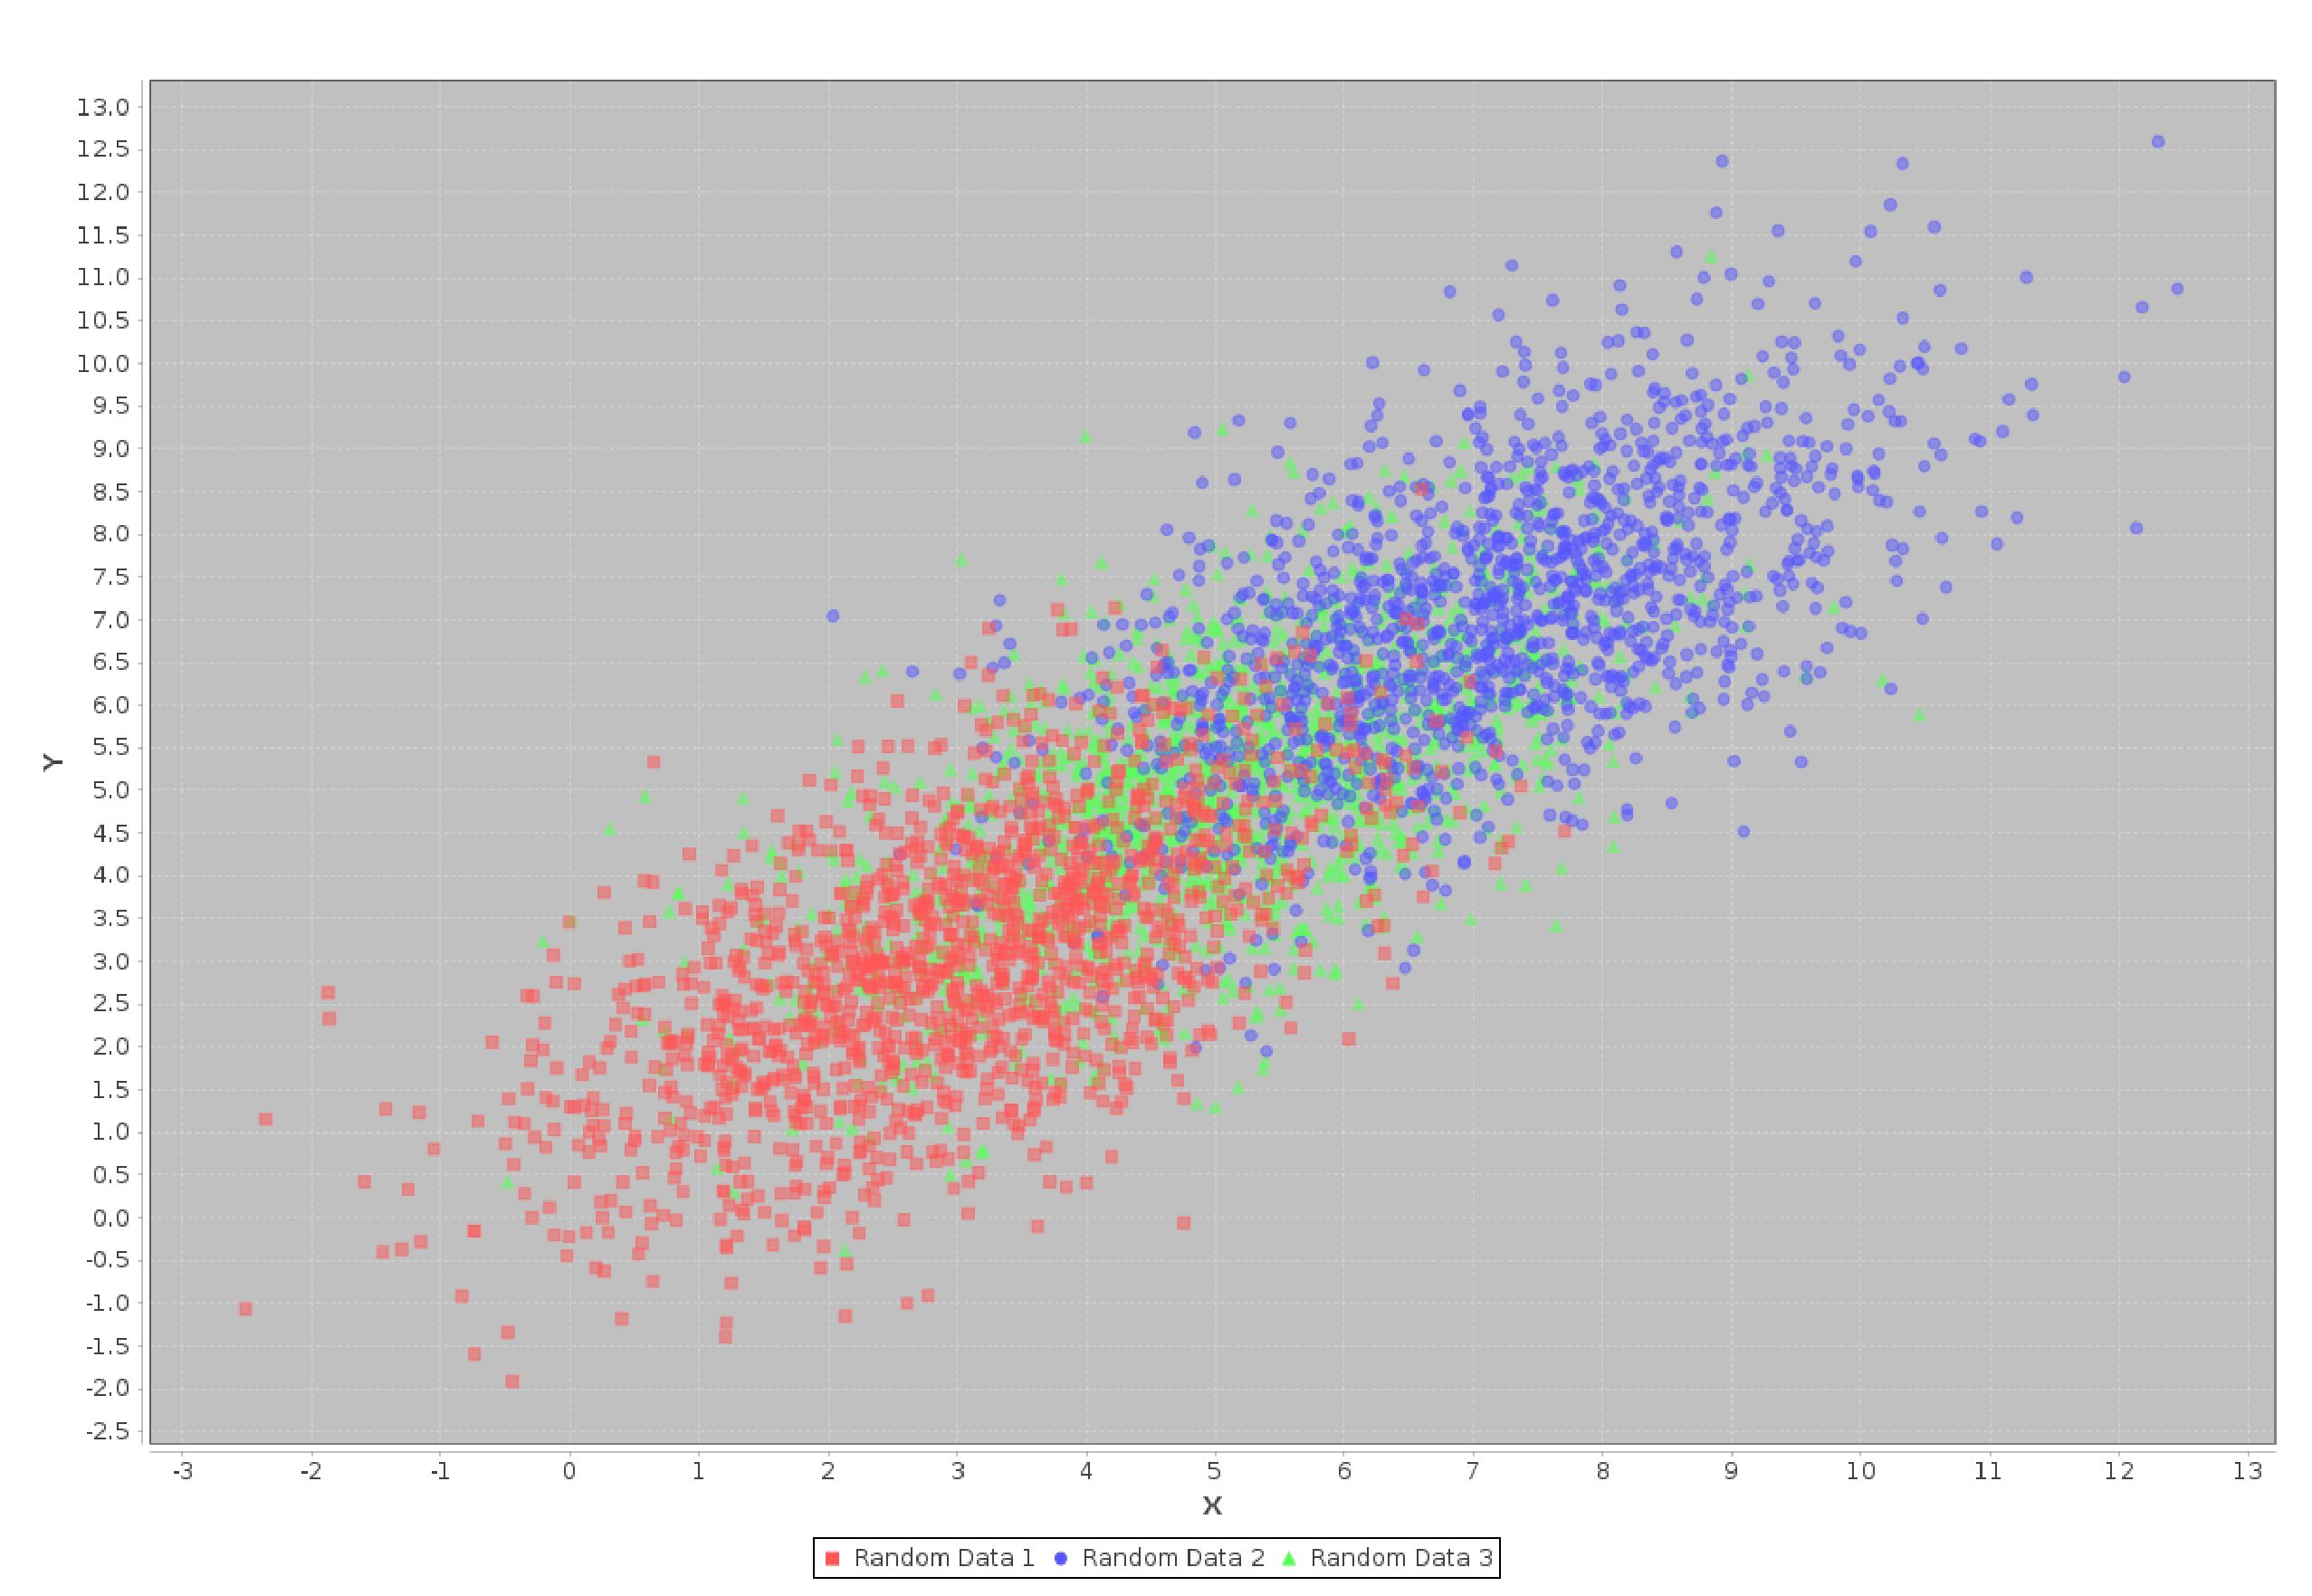
\includegraphics[width=120mm,scale=0.7]{images/dist1500-1500-5.eps}
  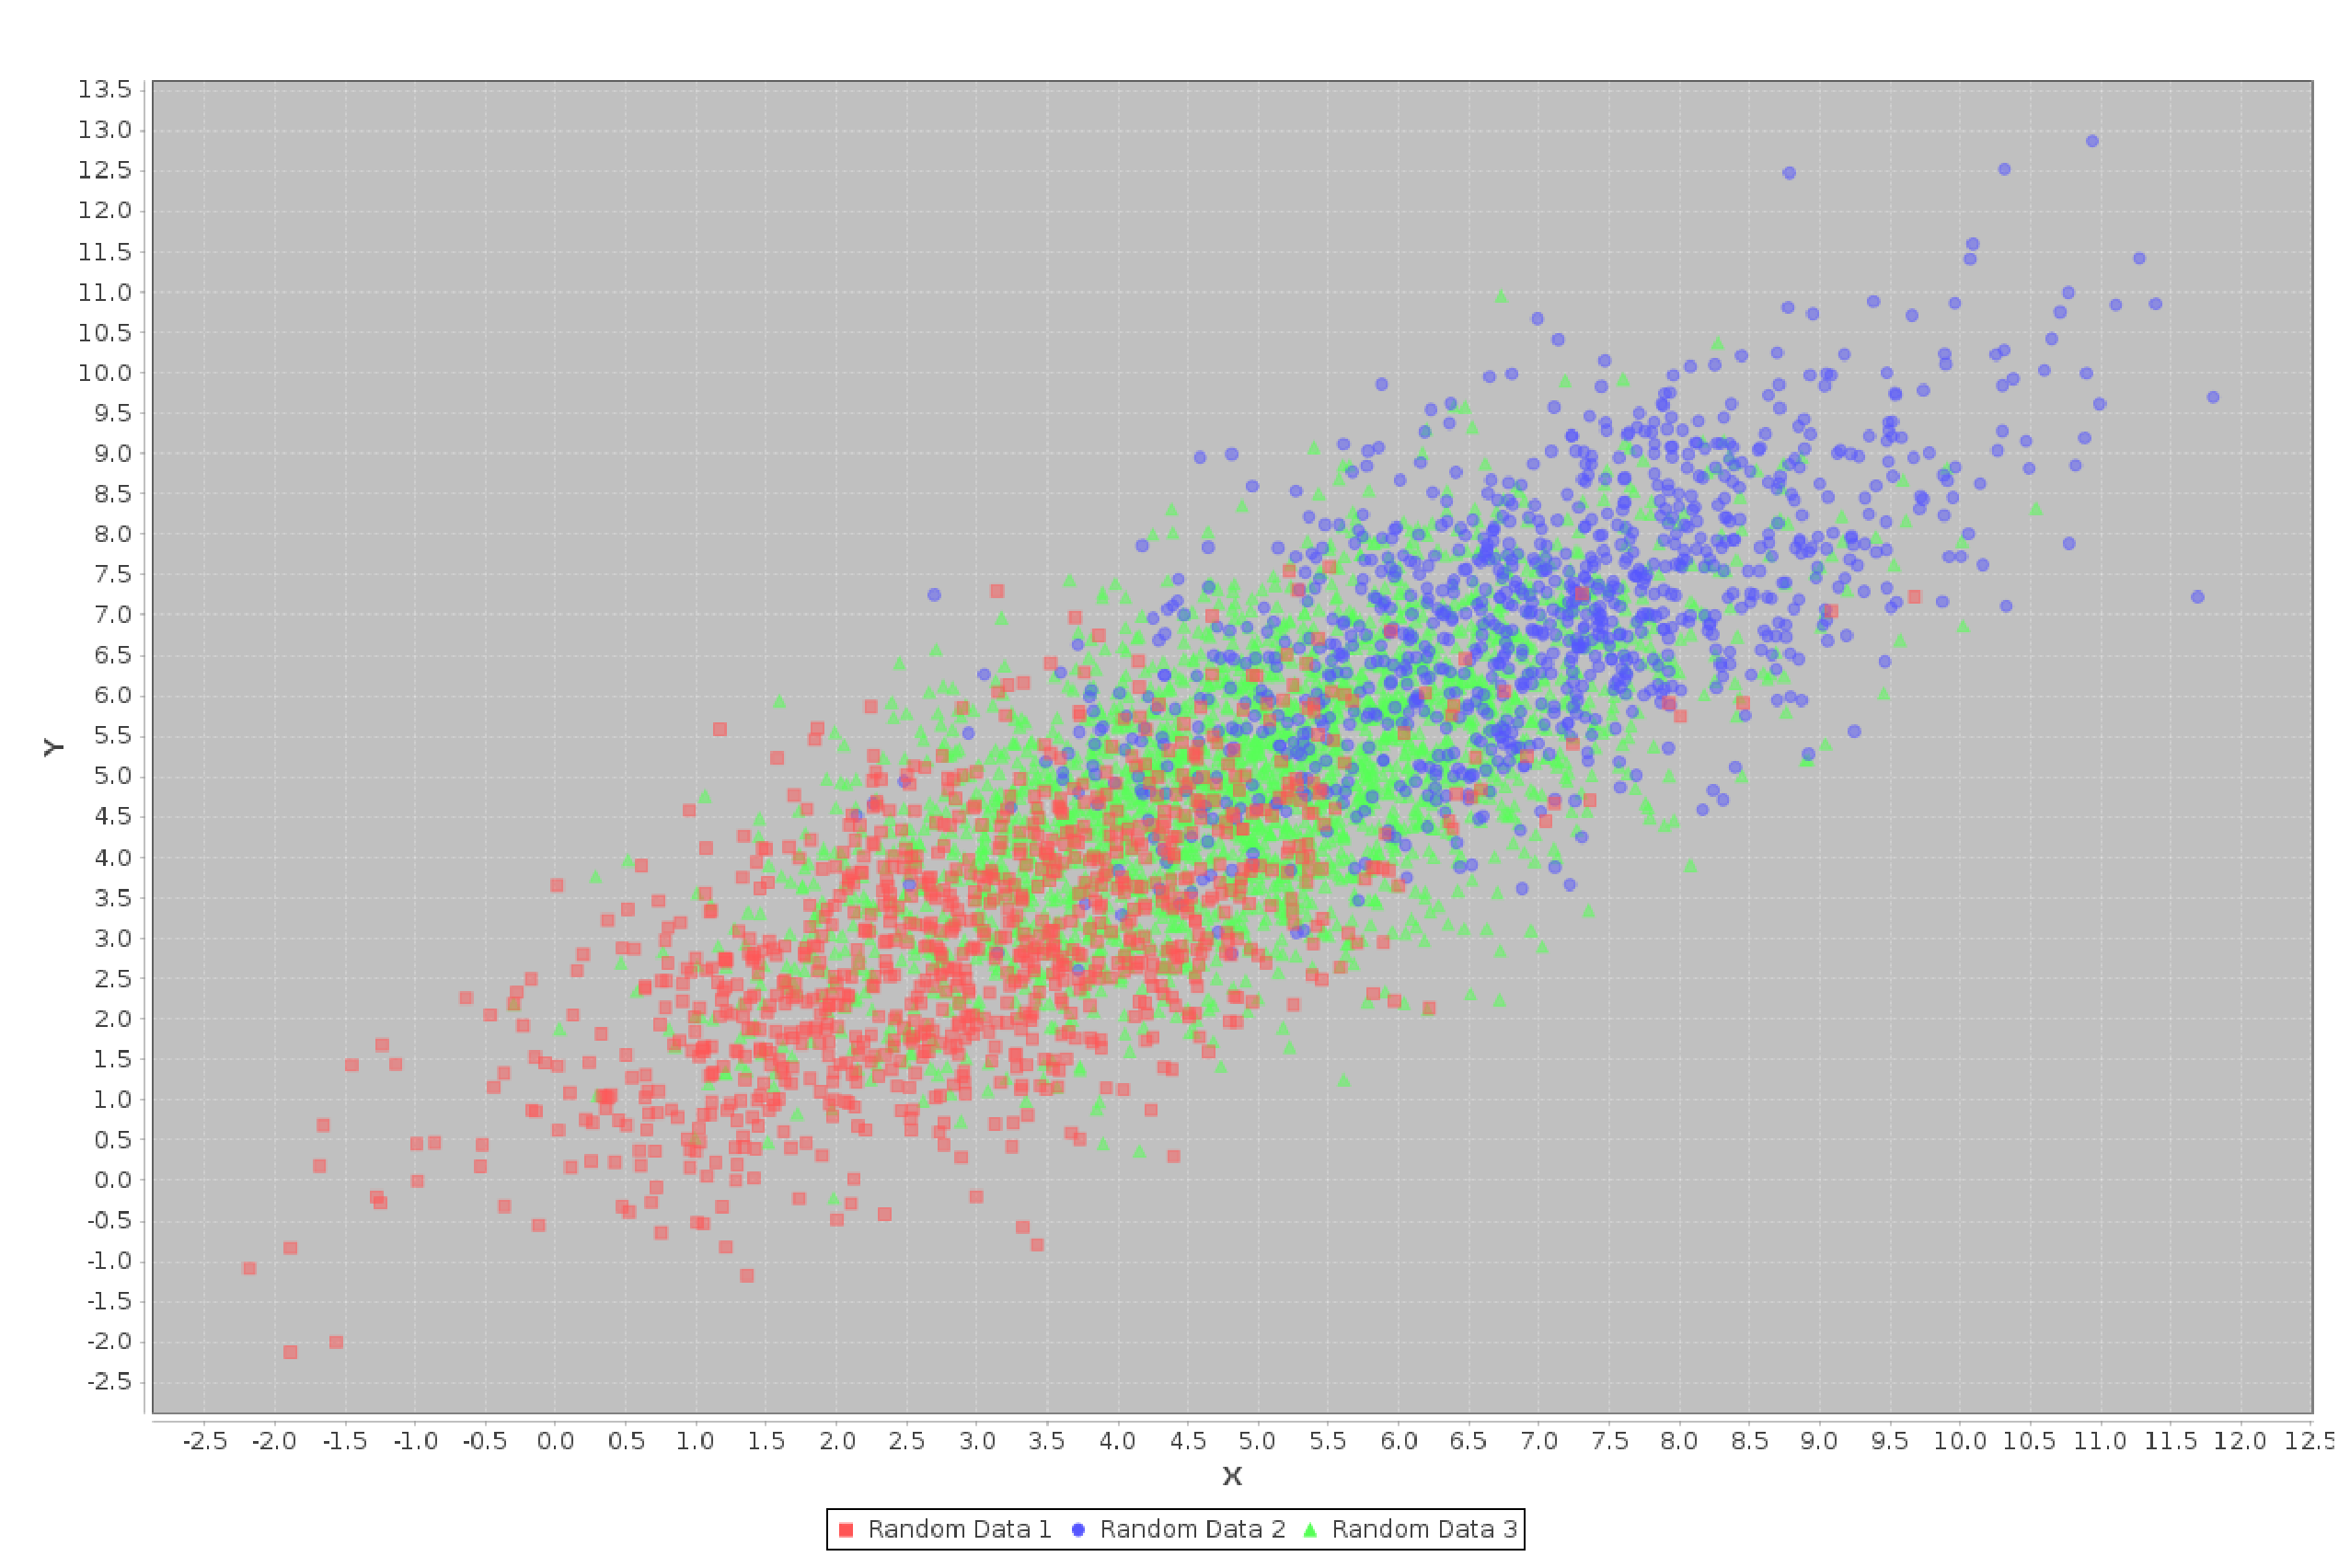
\includegraphics[width=120mm,scale=0.7]{images/dist1000-2500-5.eps}
  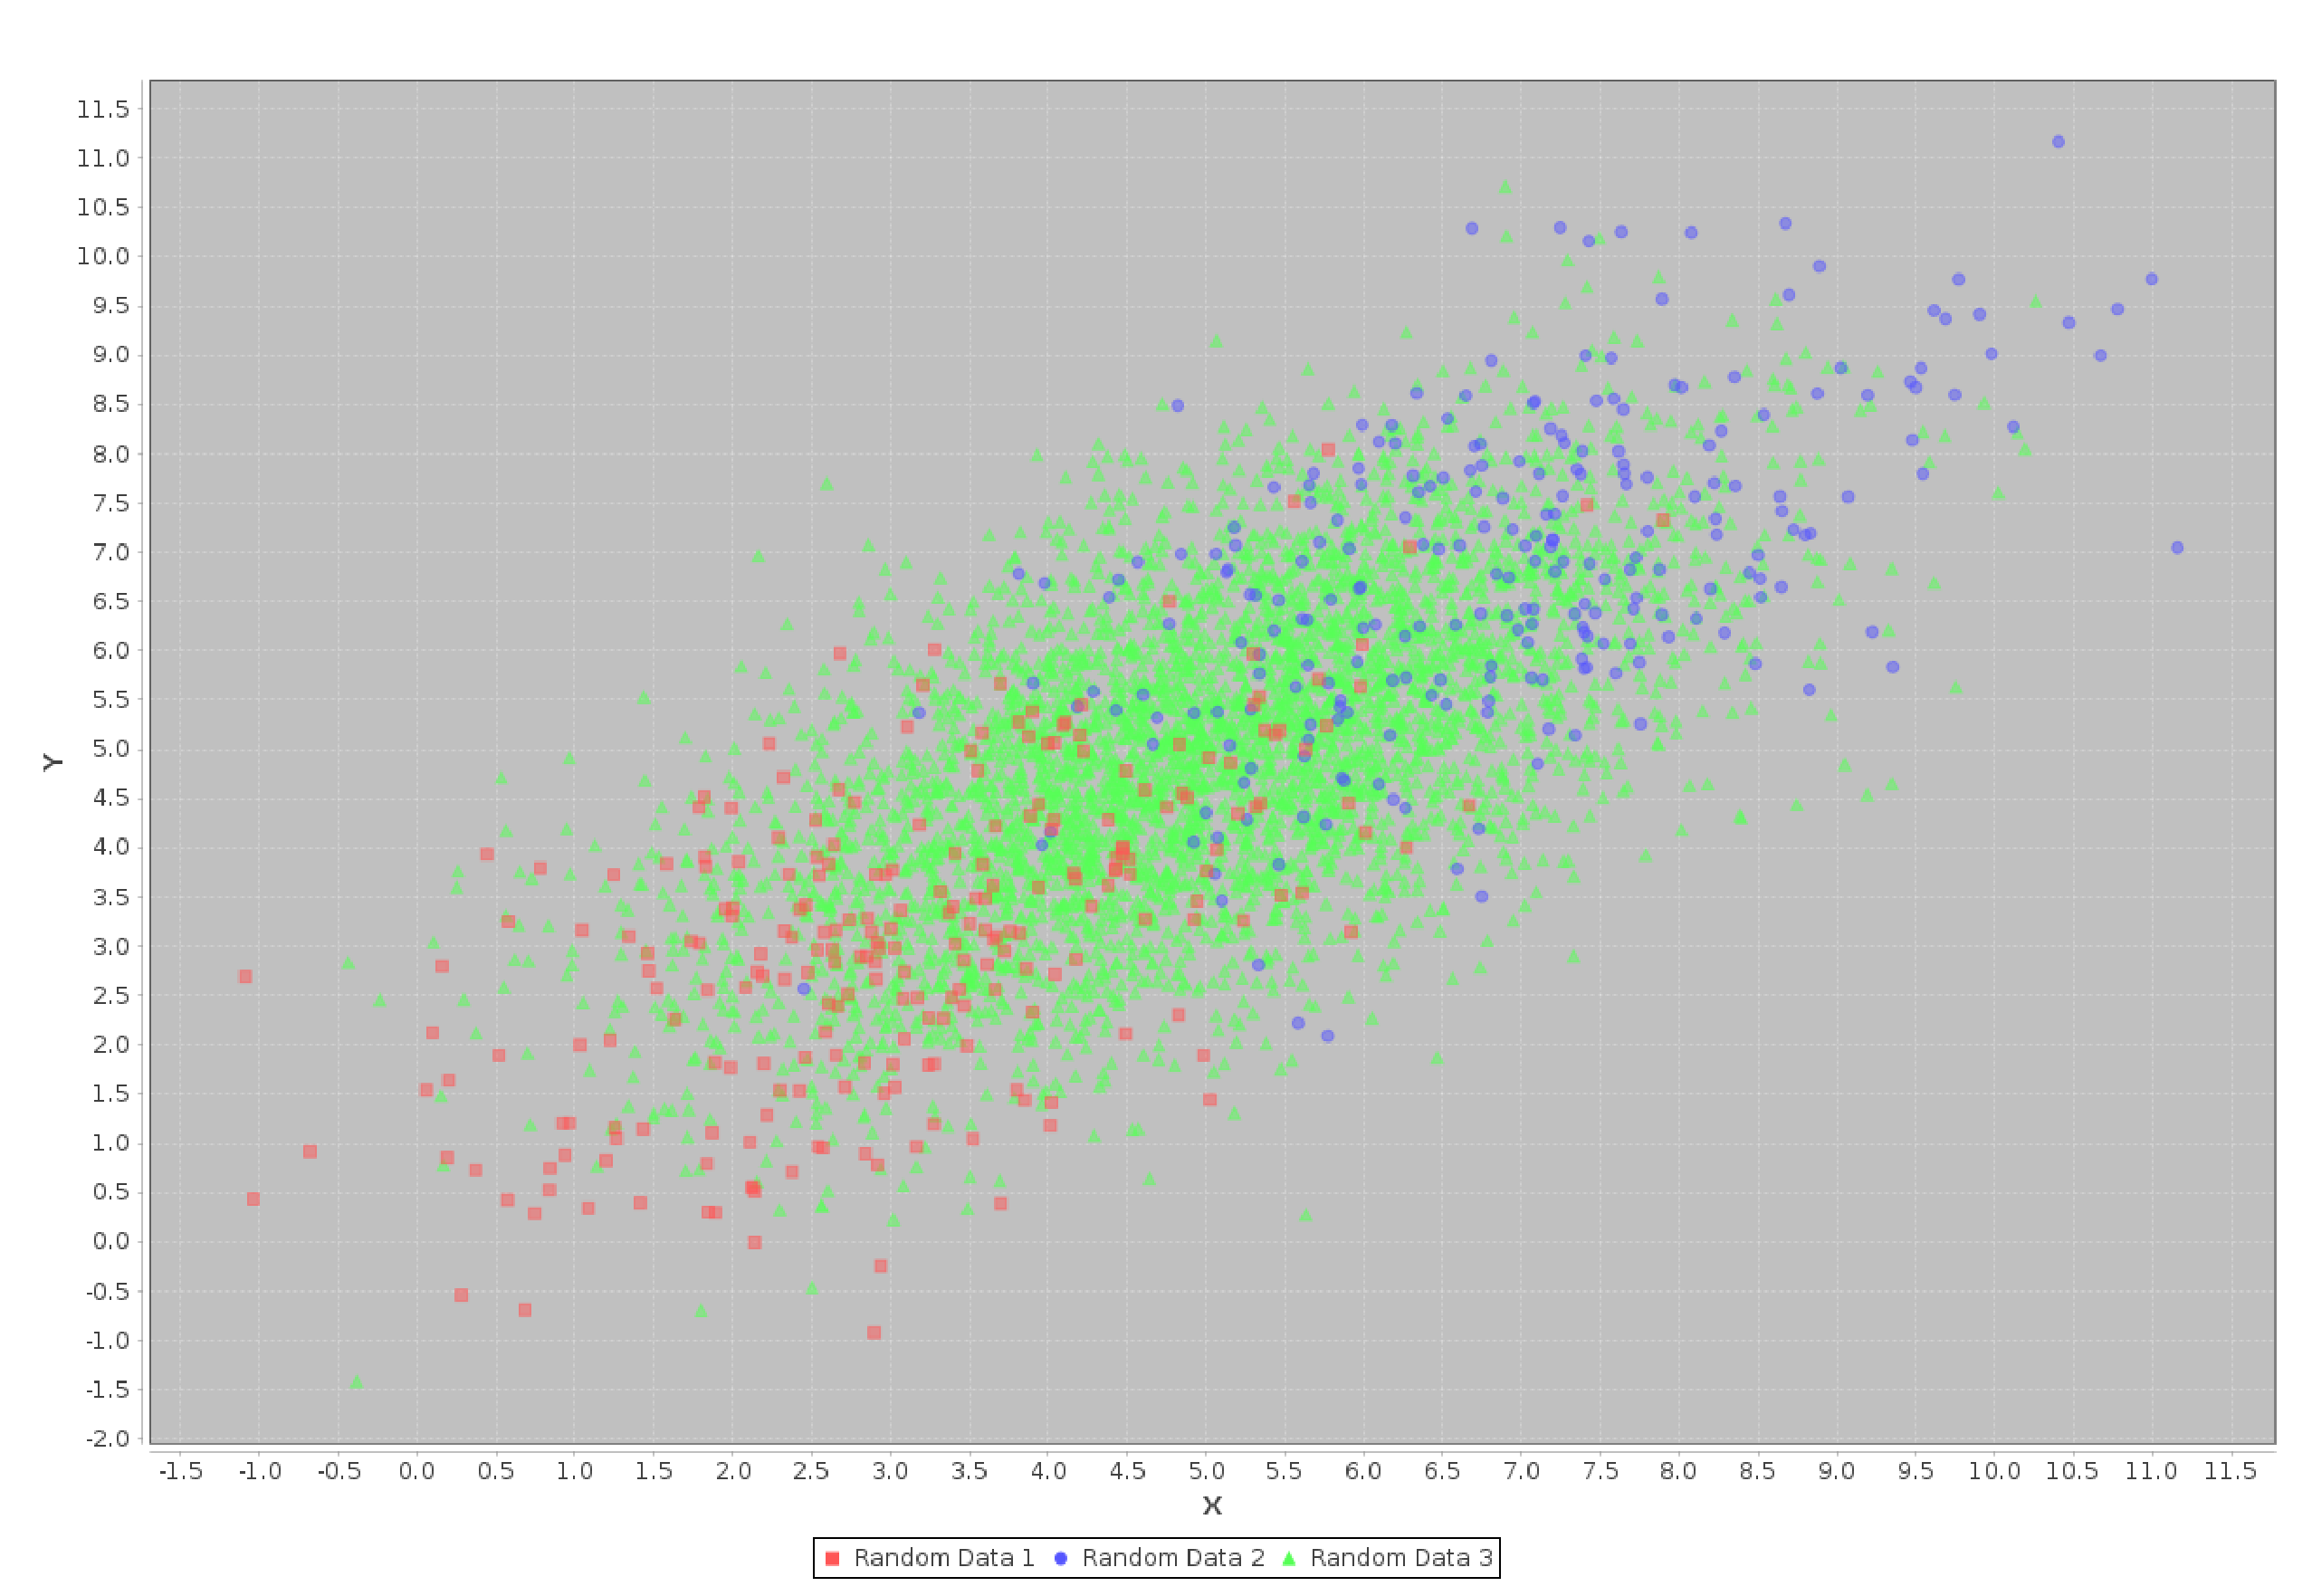
\includegraphics[width=120mm,scale=0.7]{images/dist250-4000-5.eps}
  \caption{Conjuntos de dados sintéticos com diferentes quantidades de instâncias de cada classe}
  \label{fig:dist_diferentes}
\end{figure}

Todos os conjuntos de dados criados tem 4500 pontos.
Entretanto versões com proporções diferentes de instâncias das classes foram criadas: \textit{balanceado}, \textit{normal} e \textit{desbalanceado}.
A tabela \ref{tab:dados_sinteticos} mostra as quantidades de instâncias de classes para as diferentes versões de dados.
A Figura \ref{fig:dist_diferentes} apresenta um conjunto de dados de cada versão.
Note que os três conjuntos de dados da Figura tem quantidades diferentes de instâncias de cada classe.
Todavia as médias das distribuições de cada classe nos diferentes conjuntos de dados são as mesmas.

\begin{table}[h!]
  \begin{center}
    \begin{tabular}{cccc}
      \hline
      \textbf{Conjunto de Dados} & \textbf{Verde} & \textbf{Azul} & \textbf{Vermelho}\\
      \hline

Balanceado (B)	&	 1500 & 1500 & 1500	\\
Normal (N)	&	 2500 & 1000 & 1000	\\
Desbalanceado (D)      & 4000 & 250 & 250	\\

      \hline
    \end{tabular}
    \caption{Versões de quantidades de instâncias de cada classe}
    \label{tab:dados_sinteticos}
  \end{center}
\end{table}

Além disso, os conjuntos de dados com a mesma distribuição também foram gerados em três versões diferentes.
Estas versões se diferenciam pelo posicionamento relativo das distribuições de classes: \textit{próxima}, \textit{adjacente} e \textit{distante}.
A Figura \ref{fig:dist_iguais} ilustra essas três versões para o conjunto de dados \textit{desbalanceado}.
Note que na versão \textit{próxima} a média da classe dominante (verde) está entre as médias das outras duas classes.
Nas versões \textit{adjacente} e \textit{distante} a média da classe dominante é afastada sucessivamente das outras duas classes.

\begin{figure}
  \centering
  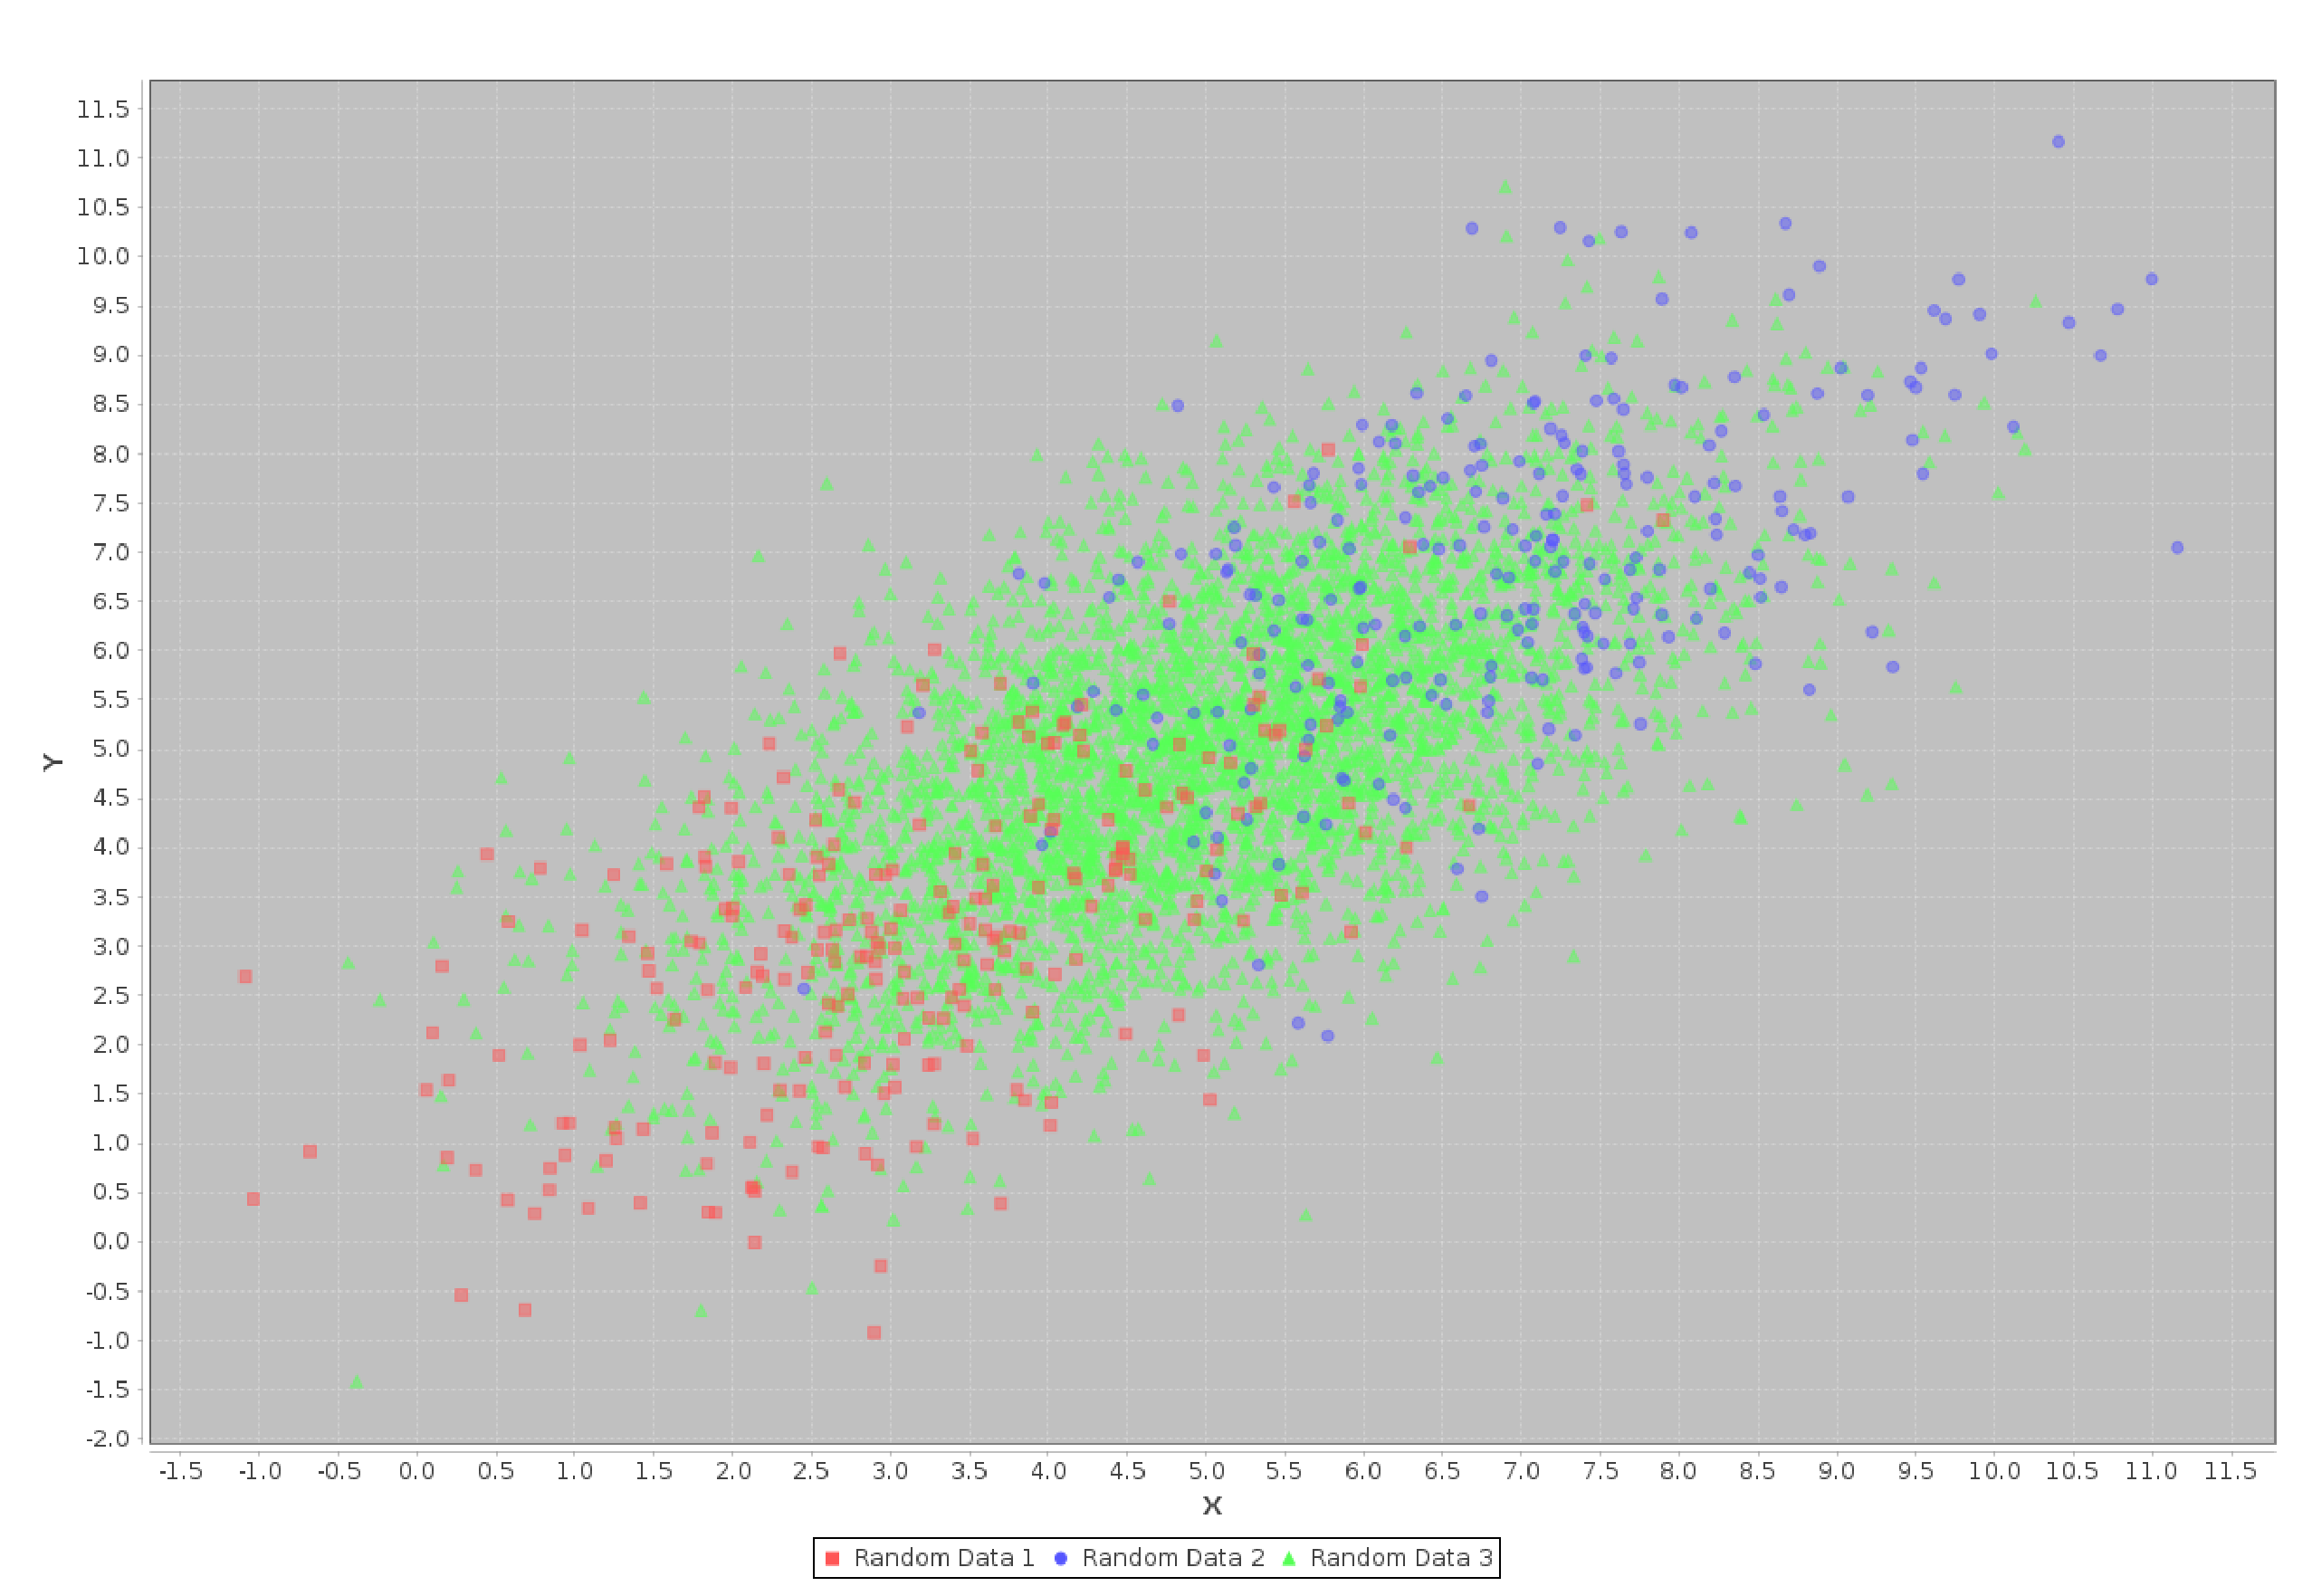
\includegraphics[width=120mm,scale=0.7]{images/dist250-4000-5.eps}
  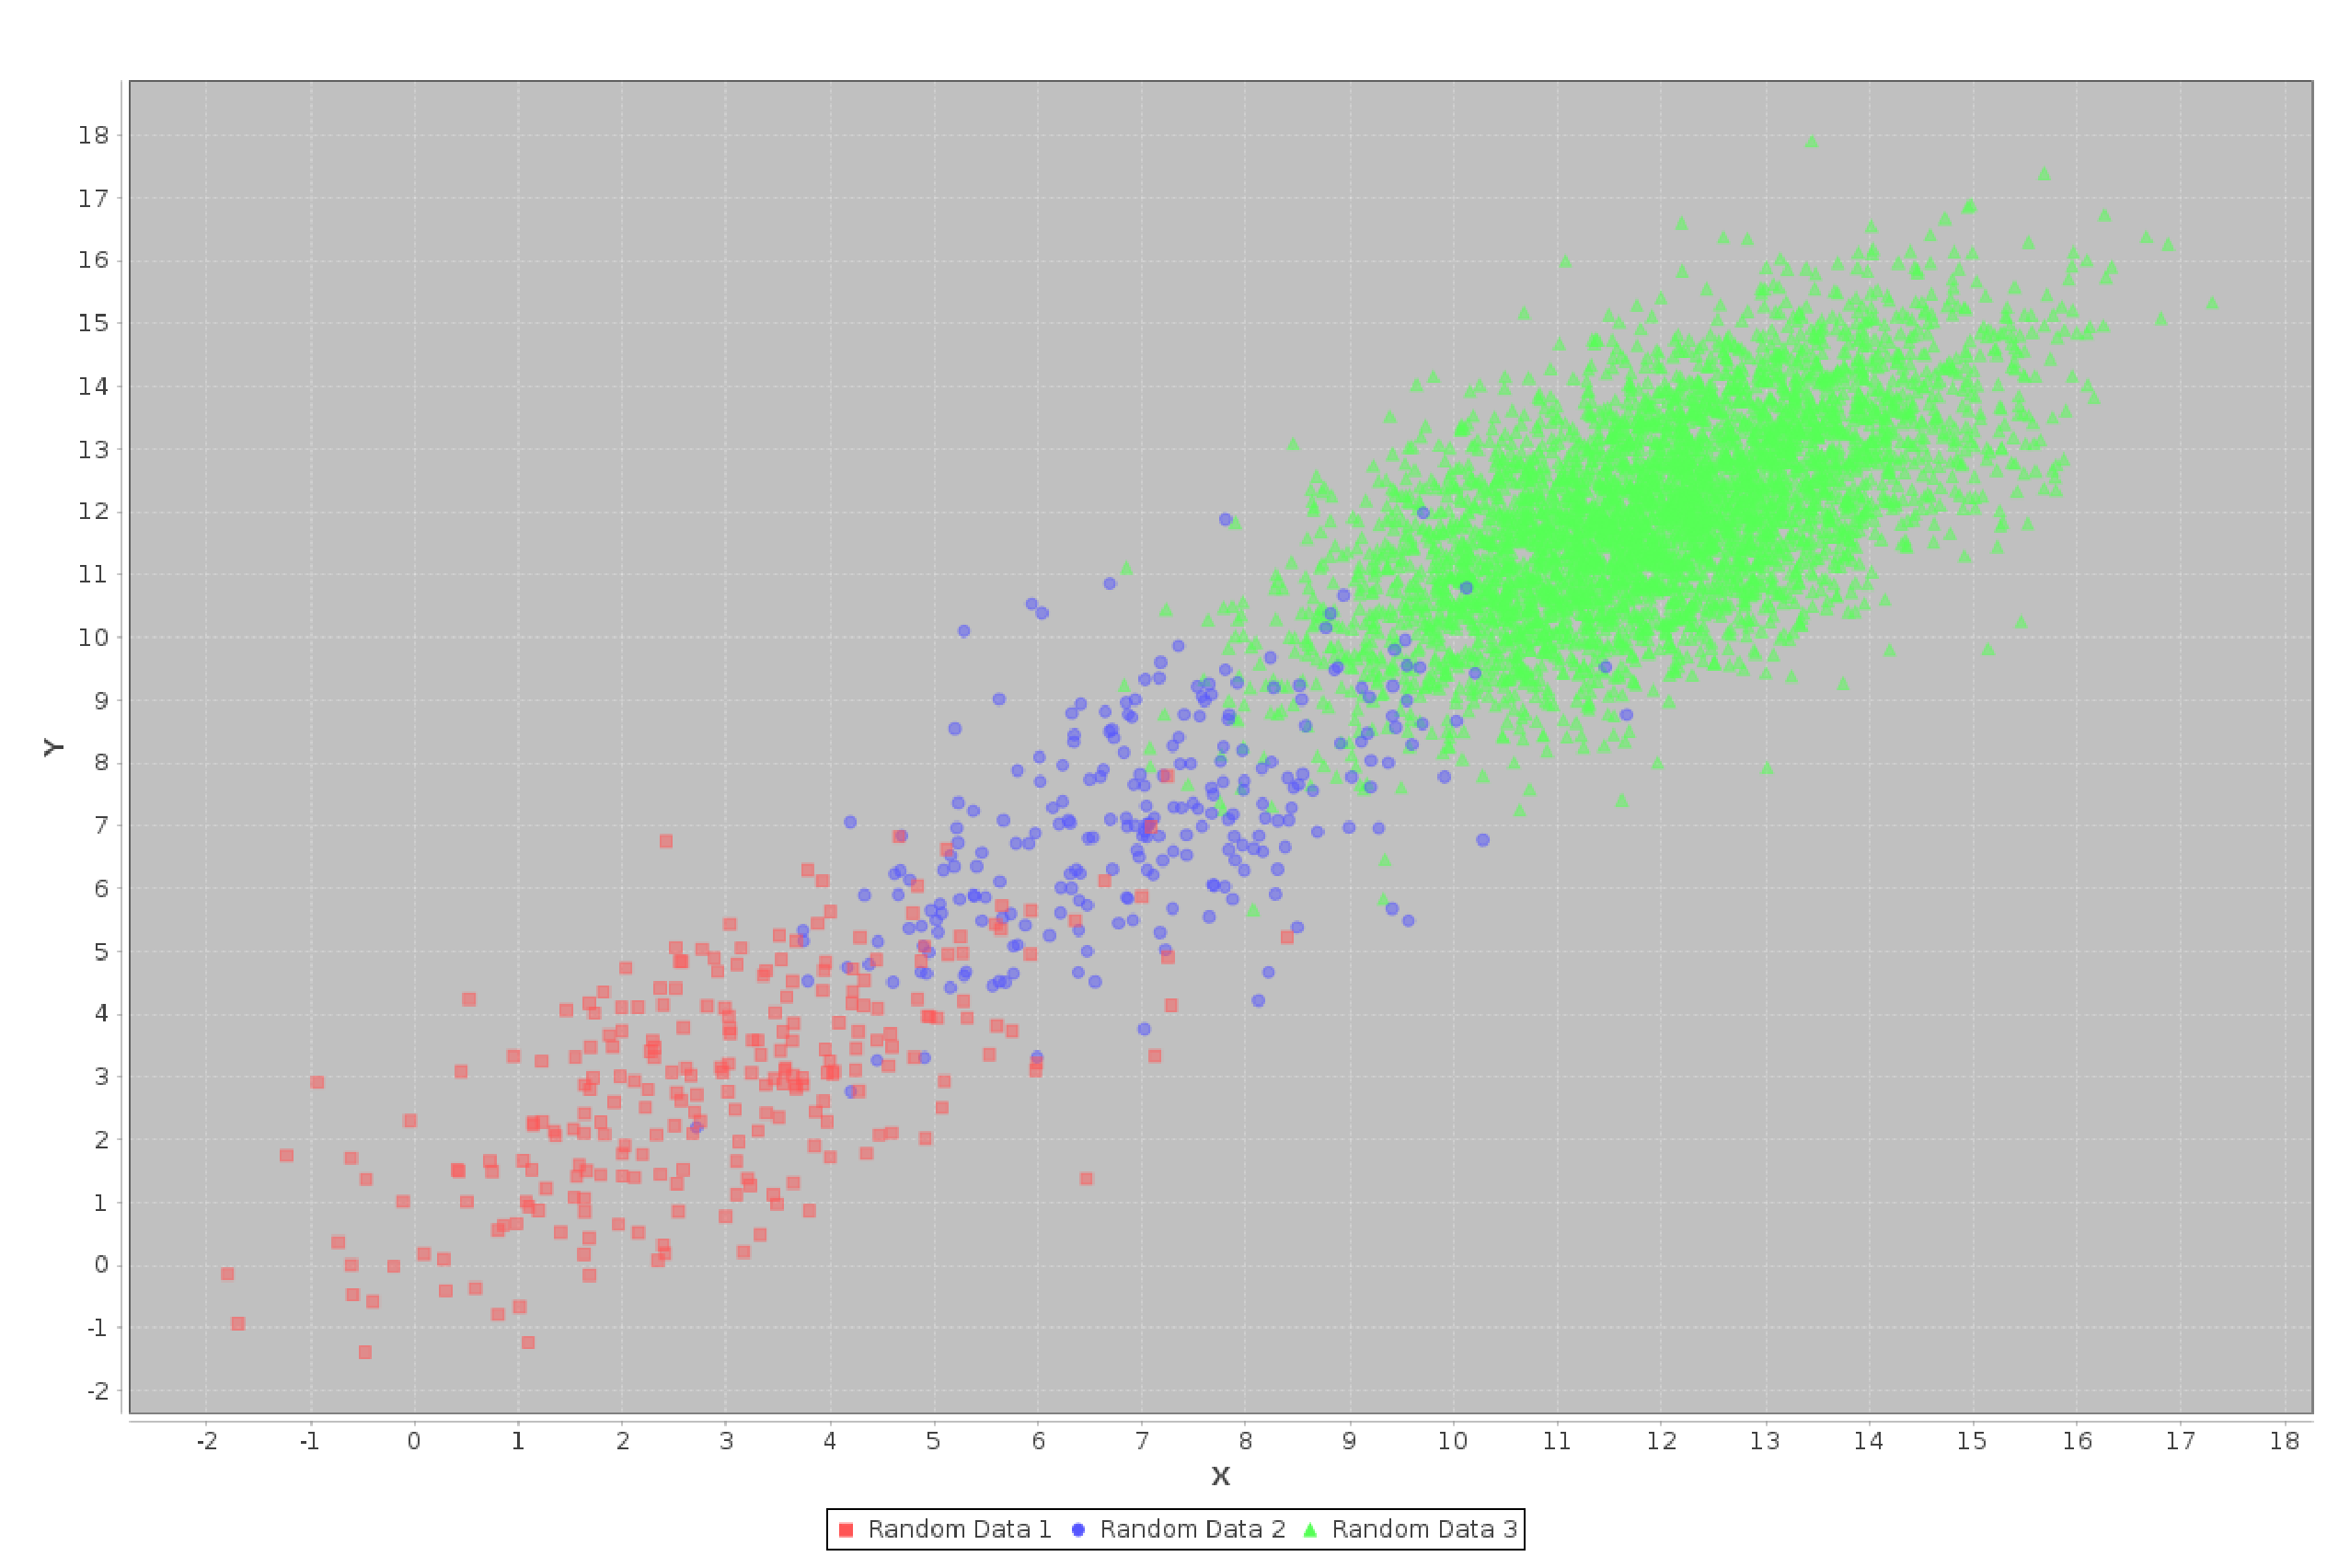
\includegraphics[width=120mm,scale=0.7]{images/dist250-4000-12.eps}
  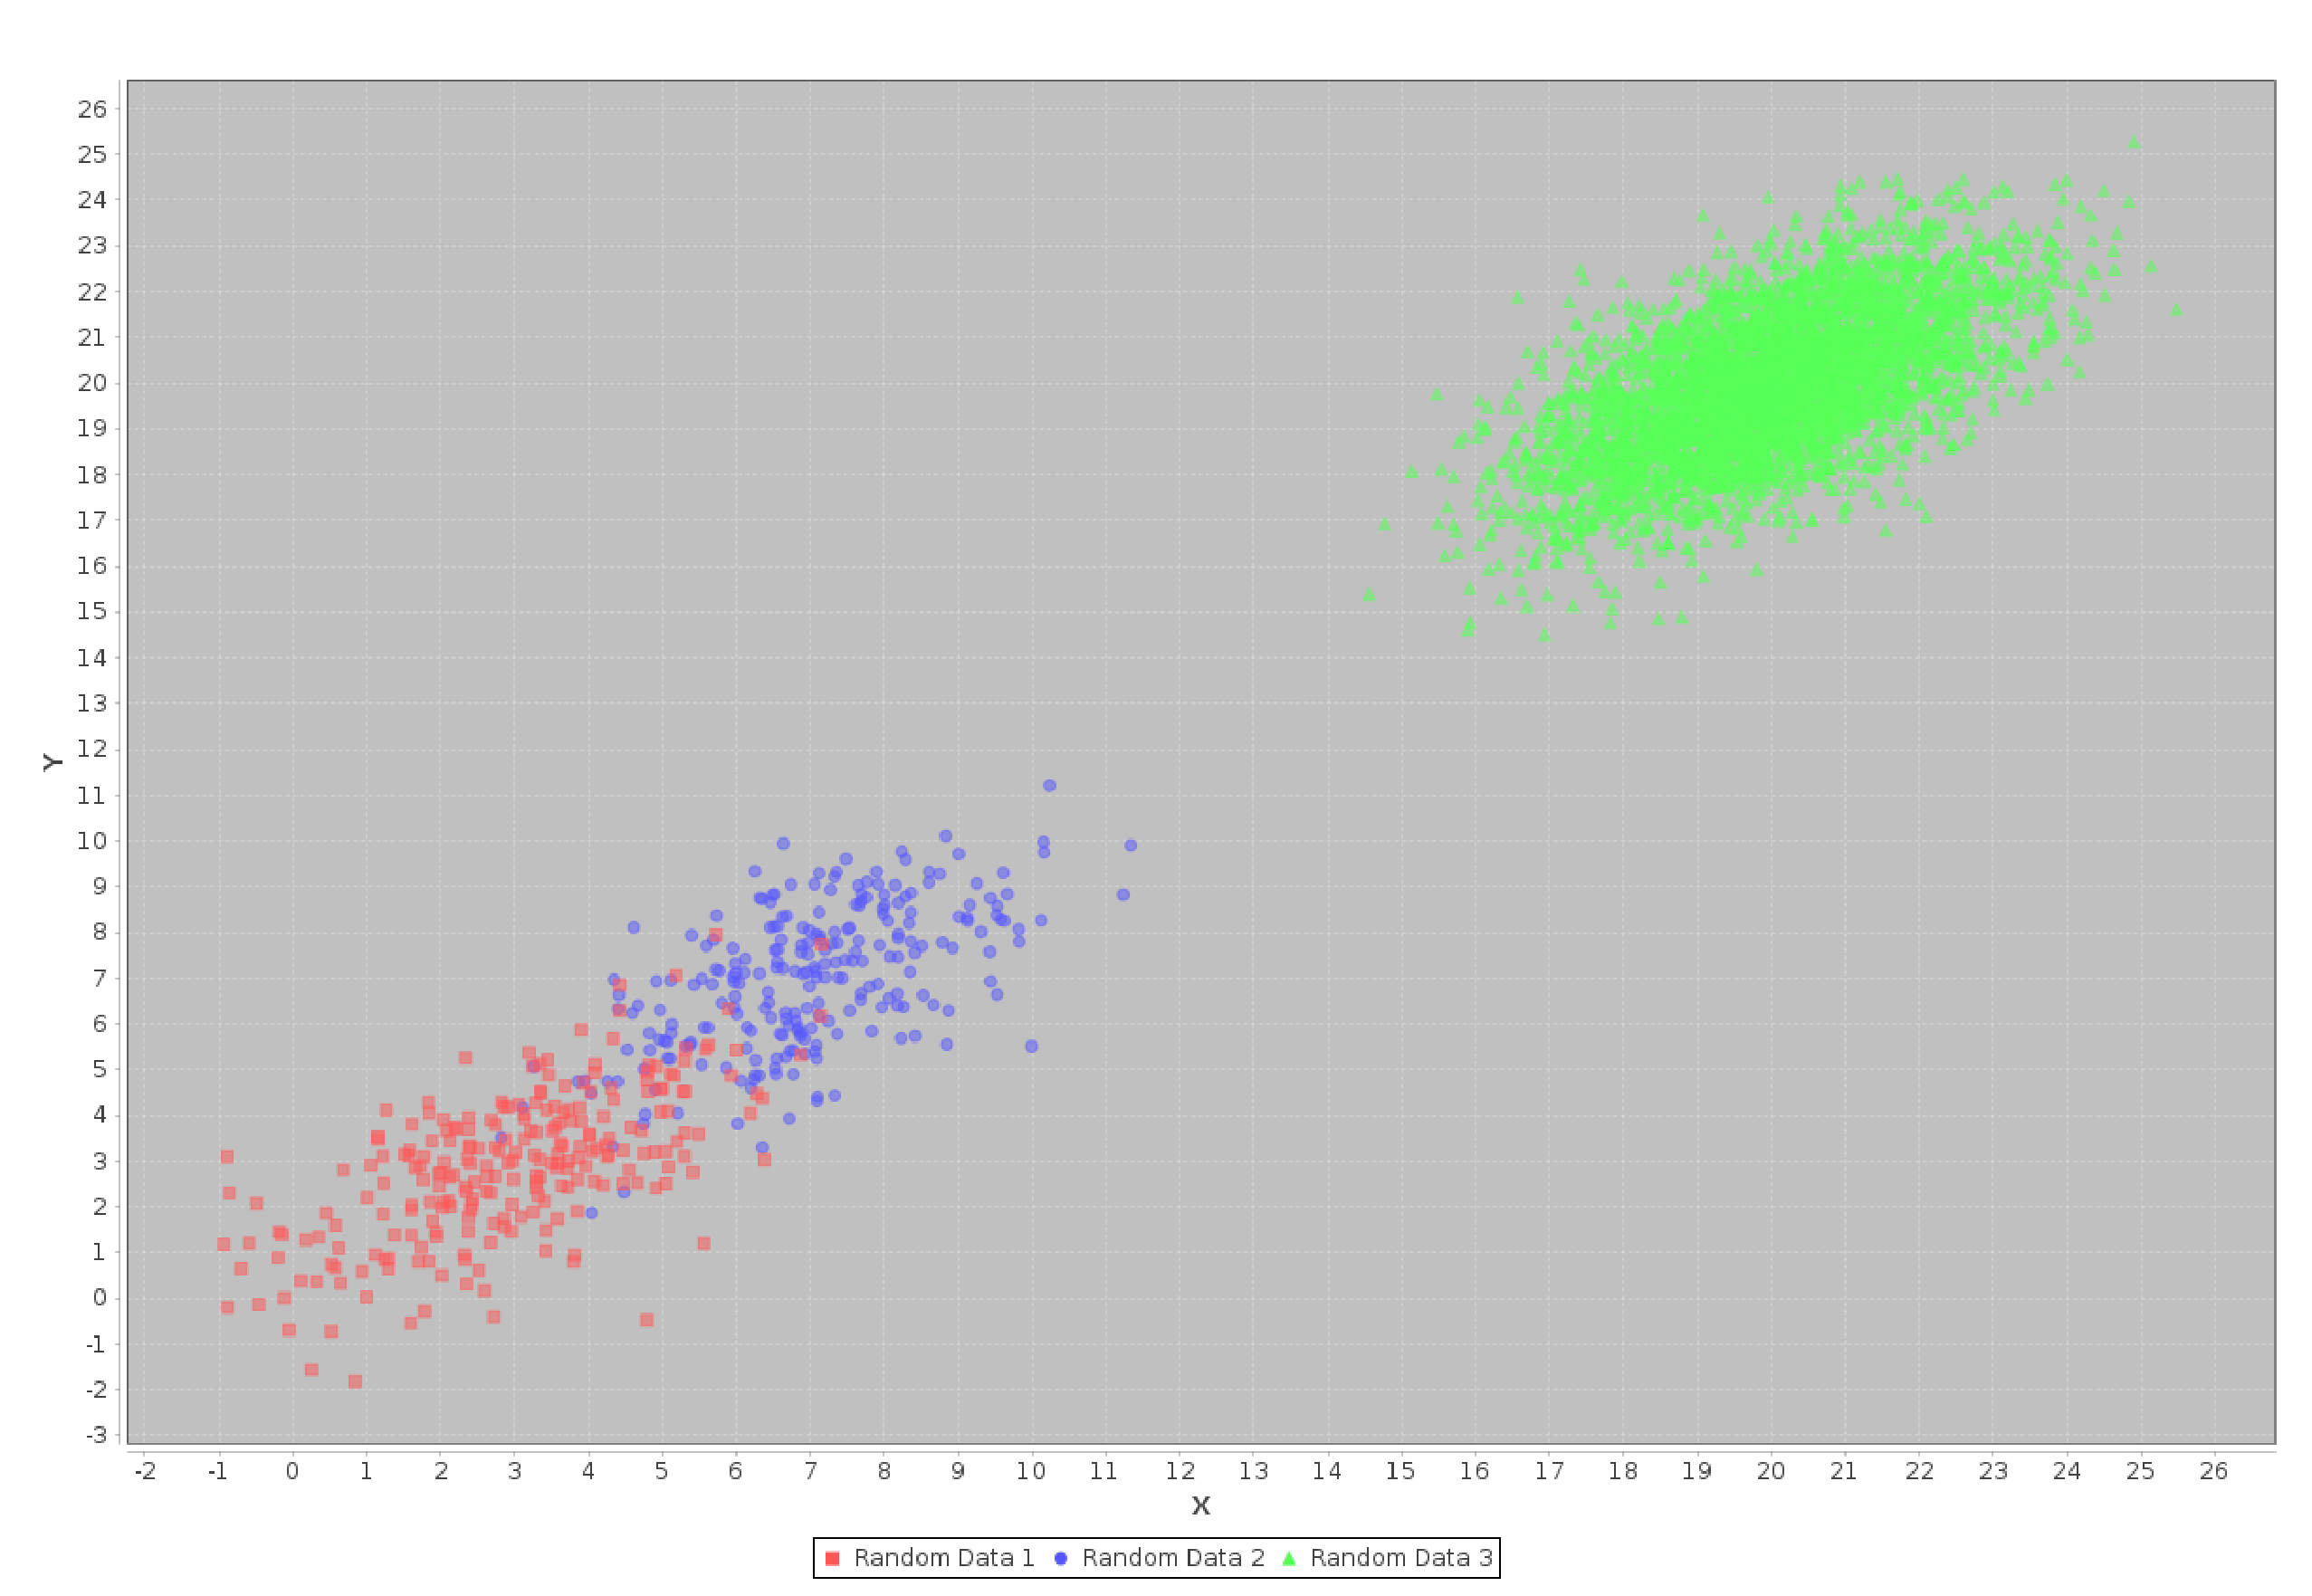
\includegraphics[width=120mm,scale=0.7]{images/dist250-4000-20.eps}
  \caption{Conjuntos de dados sintéticos com a média da distribuição da classe dominante (verde) deslocada}
  \label{fig:dist_iguais}
\end{figure}

\subsection{Resultados dos Testes com os Dados Sintéticos}

Utilizamos nove conjuntos de dados sintéticos diferentes nos testes apresentados nesta seção.
Cada conjunto combina a característica \textit{balanceado}, \textit{normal} ou \textit{ desbalanceado} com uma das configurações de posições de distribuições de classe \textit{próxima}, \textit{adjacente} ou \textit{distante}.
Com isso pudemos testar o comportamento do método de duas formas.
Na primeira verificamos como o método reage à variações no balanceamento entre classes.
Na segunda estudamos a influência da posição das distribuições de classes, i.e. elas podem estar sobrepostas, ter apenas uma interseção parcial ou serem totalmente disjuntas.

Para medir os resultados utilizamos as mesmas métricas \textit{k-Acurácia}, \textit{k-Precision} e \textit{k-Recall} apresentadas anteriormente.
Lembre que essas duas últimas vem em três tipos \textit{Micro}, \textit{Ponderada} (média ponderada das classes) e \textit{Macro} (média aritmética das classes).

Separamos na Tabela \ref{tab:ganho_meta} alguns dos resultados de destaque encontrados durante os experimentos com dados sintéticos.
É importante notar que os números apresentados nesta tabela são as diferenças entre os resultados do metaclassificador e do classificador simples.
Portanto um resultado positivo significa que o método superou o \textit{benchmark} por um percentual com aquele valor.

Como vimos anteriormente o \textit{Micro Precision} e o \textit{Micro Recall} sempre são iguais.
Além disso, o \textit{Precision Ponderado} e o \textit{Recall Ponderado} tem valores muito próximos das versões \textit{Micro}.
Portanto não apresentamos todas as métricas na tabela \ref{tab:ganho_meta}, apenas aquelas que foram mais informativas neste teste.

Os resultados apresentados na Tabela \ref{tab:ganho_meta} se referem à testes conduzidos com conjuntos de dados cuja posição das distribuições das classes era \textit{próxima}.
De fato os centros das distribuições de classes nesses conjuntos de dados são \textit{vermelha} = (3,3), \textit{verde} = (5,5) e \textit{azul} = (7,7).
A partir disso, variamos o balanceamento entre as classes ao longo do teste.
A Tabela \ref{tab:ganho_meta} identifica se os dados são balanceados (B), normais (N) ou desbalanceados (D), conforme foi detalhado na seção \ref{sub:descsinteticos}.

\begin{table}[h!]
  \begin{center}
   \resizebox{\textwidth}{!} {
   \begin{tabular}{cccccc}
      \hline
      \textbf{Algoritmo} & \textbf{Dados} &  \textbf{2-Acu.} & \textbf{2-Prec./Rec.} & \textbf{2-Prec.} & \textbf{2-Rec.} \\
          &     &     & \textbf{(Micro)} & \textbf{(Macro)} & \textbf{(Macro)} \\
      \hline


Árvore	&	B	&	0.24	&	0.33	&	0.32	&	0.33	\\
Árvore	&	N	&	0.99	&	0.98	&	1.45	&	1.45	\\
Árvore	&	D	&	1.04	&	1.04	&	6.8	&	6.27	\\
KNN 5	&	B	&	3.46	&	8	&	7.92	&	8	\\
KNN 5	&	N	&	2.78	&	4.27	&	5.41	&	4.4	\\
KNN 5	&	D	&	1.69	&	1.73	&	7.06	&	9.9	\\
KNN 7	&	B	&	7.32	&	10.58	&	8.53	&	9.01	\\
KNN 7	&	N	&	-0.41	&	-0.67	&	-0.97	&	-0.78	\\
KNN 7	&	D	&	-0.38	&	0	&	0	&	0	\\
KNN 9	&	B	&	1.64	&	4.29	&	4.29	&	4.29	\\
KNN 9	&	N	&	1.12	&	2	&	2.48	&	2.58	\\
KNN 9	&	D	&	1.04	&	1	&	4.61	&	5.88	\\
R. Forest	&	B	&	0.99	&	1.64	&	1.64	&	1.64	\\
R. Forest	&	N	&	0.53	&	0.84	&	1	&	1.09	\\
R. Forest	&	D	&	0.67	&	0.62	&	3.37	&	3.61	\\

      \hline
    \end{tabular}
    }
    \caption{Valores percentuais de ganho do Metaclassificador em relação ao \textit{Benchmark}}
    \label{tab:ganho_meta}
  \end{center}
\end{table}

É possível observar na Tabela \ref{tab:ganho_meta} que o algoritmo \textit{Árvore de Decisão } ganha por uma margem maior que 6\% no \textit{2-Precision Macro} e no \textit{2-Recall Macro} quando os dados são \textit{desbalanceados}.
Em contraste, neste mesmo cenário, o ganho é de apenas 1\% para as métricas \textit{2-Acurácia}, \textit{2-Precision Micro} e \textit{2-Recall Micro}.

Note entretanto que essas últimas métricas não tratam todas as classes do conjunto de dados por igual.
A Acurácia é uma medida geral do desempenho do modelo que simplesmente avalia a quantidade de instâncias corretamente classificadas.
Enquanto a versão \textit{Micro} do \textit{Precision} e \textit{Recall} contabilizam os totais de \textit{true positives}, \textit{false positives} e \textit{false negatives} para a partir destes calcularem os valores finais.
Desta forma, uma classe dominante com maior quantidade de instâncias, como é o caso da classe \tectit{verde}, tem maior influência no valor final dessas métricas.
Por outro lado, as versões \textit{Macro} do \textit{Precision} e \textit{Recall} são uma \textit{média aritmética} das métricas de cada classe.
Portanto, em um cenário com dados desbalanceados, essas últimas tem a sensibilidade para capturar de forma mais evidente as variações de desempenho do modelo para todas as classes do conjunto de dados.

Seguindo com a mesma análise das as métricas \textit{Macro Precision} e \textit{Macro Recall}, observamos ganhos em outros algorítimos além das \textit{Árvores de Decisão}.
Para algoritmo \textit{KNN 5} os ganhos foram de aproximadamente 7\% e 10\%, para o \textit{KNN 9} de 4,5\% e 6\% e para o \textit{Random Forest} de 3,5\%.
Desta forma podemos concluir que o método proposto foi eficiente para melhorar o resultado desses algorítimos em um cenário com dados desbalanceados e com distribuições de classes muito próximas.

Outro conjunto notável de resultados que podem ser vistos na Tabela \ref{tab:ganho_meta} são aqueles referentes aos dados perfeitamente balanceados.
Note que neste contexto o algoritmo \textit{KNN 5} exibe ganhos de cerca de 8\% em todas as métricas \textit{Precision} e \textit{Recall}.
Um ganho de desempenho similar, embora menor, pode ser visto nos testes com os algoritmos \textit{KNN 9} e \textit{Random Forest}.
Este cenário de testes é especial pois representa uma tarefa mais difícil para muitos algoritmos.
Lembre que neste caso as médias das distribuições das três classes do conjunto de dados estão muito próximas e portanto estas tem uma grande interseção no espaço amostral (vide primeira imagem da Figura \ref{fig:dist_diferentes}).
Este resultado demonstra que o método proposto também melhorou o desempenho desses algoritmos neste caso.

Por fim, ainda é possível observar ganhos de 3,5\% a 5,5\% no \textit{Precision} e \textit{Recall} para o algoritmo \textit{KNN 5} nos testes com dados do tipo \textit{normal}.
Recorde que estes são um meio termo entre os dados \textit{balanceados} e \textit{desbalanceados}.
Ganhos menores são observáveis na mesma situação para os algorítimos \textit{KNN 9} e \textit{Random Forest}.
Novamente este resultado reforça que o método proposto melhora o resultado desses algoritmos para conjuntos de dados cujas classes tem distribuições com médias muito próximas e que portanto se sobrepõem.

Como citamos, diversos outros testes com dados sintéticos foram feitos mas mostramos apenas os resultados de interesse nesta seção.
Realizamos os mesmos testes discutidos aqui com dados onde as distribuições das classes estão mais afastadas (\textit{adjacente} e \textit{distante}), conforme ilustrado na Figura \ref{fig:dist_iguais}.
Porém nestes demais cenários o metaclassificador não se destacou de maneira substancial.
Embora ele tenha apresentado algum ganho na maioria dos casos, estes são iguais ou inferiores a 1\%.
Para ver o restante dos resultados com os dados sintéticos consulte o apêndice desta dissertação.


\chapter{Trabalhos Relacionados}

A \textit{Classificação em Múltiplas Classes} representa um importante subgrupo das tarefas de classificação abordadas pelo aprendizado de máquina.
Diferente dos problemas clássicos de classificação, neste caso cada instância está associada à mais de uma classe \cite{Tsoumakas}.
Além disso, é possível que as classes tenham correlações entre si de forma a influenciar no resultado final, aumentando a dificuldade da tarefa.
De maneira formal, a tarefa de classificação em múltiplas classes requer que o vetor de atributos de entrada \textit{x} seja mapeado em um vetor de saída \textit{y} com valores binários que representam as classes.
Isto é, \textit{x} é da forma $[a_1, a_2, ..., a_n]$, onde $a_j$ representa um dos n atributos, e \textit{y} da forma $[c_1, c_2, ... , c_k]$ onde $c_j$ pode assumir o valor zero ou um, indicando se aquela classe está relacionada à instância.  

O método proposto nesta dissertação figura entre diversos outros que procuram solucionar problemas de classificação em múltiplas classes.
Ainda mais especificamente aqueles voltados para \textit{ranking}, que é uma das tarefas cada vez mais proeminentes em aprendizado supervisionado.

Entre as soluções encontradas na literatura podemos destacar ainda aquelas que fazem a transformação do problema \cite{Tsoumakas}.
Isto é, elas executam uma transformação do problema de classificação em múltiplas classes de forma que ele possa ser solucionado com uma ou mais classificações em uma classe.
Como o método proposto nesta dissertação também se baseia em transformação do problema (filtragens sucessivas do conjunto de dados), a seguir apresentaremos alguns destes métodos.

O método de transformação de problema mais famoso é chamado de \textit{Binary Relevance} \cite{Tsoumakas, Godbole, Zhang}.
Este método se baseia em transformar um problema de classificação em múltiplas classes em diversos problemas de classificação binários.
Ou seja, se existem $\vert L \vert$ classes diferentes no conjunto de dados, $\vert L \vert$ classificadores diferentes são treinados.
Cada um deles é responsável pela classificação binária referente à uma das $\vert L \vert$ classes do conjunto de dados.
Note porém que este método não é capaz de modelar qualquer tipo de correlação entre as classes, portanto não pode ser usado para gerar listas ordenadas por relevância.

\textit{Label Powerset} é mais um método clássico encontrado na literatura \cite{Tsoumakas02, Read02}.
Este método se baseia em transformar cada possível combinação entre as $\vert L \vert$ classes em novas classes atômicas.
Com isso o problema pode ser resolvido por um classificador para múltiplas classes comum.
Além disso, este método leva diretamente em consideração a coorelação entre classes.
Todavia, a desvantagem do \textit{Label Powerset} é sua complexidade de tempo no pior caso.

Outro método, baseado em \textit{Label Powerset}, é chamado \textit{RAkEL} (\textit{RAndom k labELsets}) \cite{Tsoumakas03}.
Sua proposta é segmentar aleatoriamente o conjunto de dados de acordo com as classes.
Desta forma diversos subgrupos menores (\textit{labelsets}) podem ser criados.
Estes subgrupos também podem ou não ter classes em comum.
Um classificador é treinado para cada subgrupo utilizando o método \textit{Label Powerset} citado anteriormente.
Para classificar uma nova instância o método combina os resultados de todos os classificadores.

Existem diversos métodos que transformam um conjunto de dados com múltiplas classes por exemplo em outro com uma única classe por exemplo \cite{Boutell, Chen}.
Nestes métodos a proposta é que cada exemplo (x,Y) seja decomposto em $\vert Y \vert$ exemplos (x, l) onde $l \in Y$.
Com isso um único classificador probabilístico pode ser treinado por meio do conjunto de dados transformado.
É possível então classificar uma nova instância a partir da distribuição de probabilidades devolvida por tal classificador.
As classes pertinentes podem ser selecionadas entre aquelas com probabilidade superior a um dado patamar, e.g. 50 \%.

Entre os modelos de transformação de problema também podemos citar o de classificadores em cascata \cite{Read}. 
No caso de um conjunto de dados D com $\vert L \vert$ valores de classe diferentes, $\vert L \vert$ classificadores são utilizados em cascata. 
O conjunto de dados de cada classificador é acrescido sucessivamente de um novo atributo binário, que informa o resultado do classificador anterior. 
Com isso os classificadores em cascata são capazes de utilizar, em certo nível, a informação de interdependência entre classes. 
Notadamente, a ordem dos classificadores impacta na acurácia final.
Para resolver este problema o artigo introduz o esquema de conjuntos de classificadores em cascata. 
Neste caso, subconjuntos aleatórios de D são utilizados para treinar cada classificador. 
Além disso, cada classificador é treinado com uma ordem aleatória de classes. 
Ao classificar um novo exemplo a lista de saída é dada pela votação por comitê. 
Desta forma o conjunto de classificadores em cascata é capaz de gerar um ranking diretamente.

\textit{Ranking by pairwise comparison} é um método que transforma um conjunto de dados com múltiplas classes em diversos conjuntos de dados com a classe binária \cite{Hullermeier, Mencia, Furnkranz}.
Um novo conjunto é criado para cada par de classes do conjunto de dados original.
Este encorpora os exemplos que contemplam uma classe ou a outra, mas não as duas.
Um classificador binário é então treinado para cada um desses conjuntos no intuito de aprender a diferenciar entre as duas classes em questão.
Por fim, esses classificadores são empregados em conjunto para gerar a lista ordenada de saída referente à uma nova instância.


%	Métodos para ranking?
%	Label Rankings ?


%%%%%%%%%%%%%%%%%%%%%%%%%%%%%%%%%%%%%%%%%%%%%%%%%%%%%%%%%%%%%%%%%%%%%%%%%%%%%%%%

\arial
\bibliography{thesis}

%%%%%%%%%%%%%%%%%%%%%%%%%%%%%%%%%%%%%%%%%%%%%%%%%%%%%%%%%%%%%%%%%%%%%%%%%%%%%%%%
\normalfont

\appendix

\chapter{Primeiro Apêndice}
O primeiro apêndice deve vir após as referências bibliográficas. Depois que você colocar a diretiva ``{$\backslash$}apendix'', todos os ``{$\backslash$}chapter\{\}'' vão gerar apêndices.

\end{document}
